% Retoca las líneas marcadas con TODO según las necesidades

\documentclass[oneside,a4paper,12pt]{book} % TODO: cambia "oneside" por "twoside" a la hora de imprimirlo

\usepackage[spanish]{babel}
\usepackage[utf8]{inputenc}
\usepackage{geometry}
\usepackage{makeidx}
\usepackage{url}
\usepackage{graphicx}
\usepackage{color}
\usepackage{caption}
\usepackage{acronym}
\usepackage{hyphenat}
\usepackage{a4wide}
\usepackage[normalsize]{subfigure}
\usepackage{float}
\usepackage{titlesec}
\usepackage[Lenny]{fncychap}
\usepackage{listings} % para poder hacer uso de "listings" propios (p.ej. códigos)
\usepackage{eurosym} % para poder usar el símbolo del euro con \euro {xx}
\usepackage{hyperref} % TODO: añade la opción hidelinks para imprimirlo (los enlaces no aparecerán resaltados)

% Para que no parta las palabras
\pretolerance=10000

\newcommand{\bigrule}{\titlerule[0.5mm]} \titleformat{\chapter}[display] % cambiamos el formato de los capítulos
{\bfseries\Huge} % por defecto se usaron caracteres de tamaño huge en negrita
{% contenido de la etiqueta 
\titlerule % línea horizontal 
\filright % texto alineado a la derecha 
\Large\chaptertitlename\ % capítulo e índice en tamaño large
\Large % en lugar de 
\Huge \Large\thechapter} 
{0mm} % espacio mínimo entre etiqueta y cuerpo
{\filright} % texto del cuerpo alineado a la derecha
[\vspace{0.5mm} \bigrule] % después del cuerpo, dejar espacio vertical y trazar línea horizontal gruesa
\geometry{a4paper, left=3.5cm, right=2cm, top=3cm, bottom=2cm, headsep=1.5cm}

% Estilos para ilustrar códigos:
\definecolor{code_green}{rgb}{0,0.6,0}
\definecolor{code_gray}{rgb}{0.5,0.5,0.5}
\definecolor{code_mauve}{rgb}{0.58,0,0.82}

\lstset{frame=tb,
  language=C,
  aboveskip=3mm,
  belowskip=3mm,
  showstringspaces=false,
  columns=flexible,
  basicstyle={\small\ttfamily},
  numbers=none,
  numberstyle=\tiny\color{code_gray},
  keywordstyle=\color{blue},
  commentstyle=\color{code_green},
  stringstyle=\color{code_mauve},
  breaklines=true,
  breakatwhitespace=true,
  tabsize=3
}

\lstset{frame=tb,
  language=C++,
  aboveskip=3mm,
  belowskip=3mm,
  showstringspaces=false,
  columns=flexible,
  basicstyle={\small\ttfamily},
  numbers=none,
  numberstyle=\tiny\color{code_gray},
  keywordstyle=\color{blue},
  commentstyle=\color{code_green},
  stringstyle=\color{code_mauve},
  breaklines=true,
  breakatwhitespace=true,
  tabsize=3
}

\lstset{frame=tb,
  language=Python,
  aboveskip=3mm,
  belowskip=3mm,
  showstringspaces=false,
  columns=flexible,
  basicstyle={\small\ttfamily},
  numbers=none,
  numberstyle=\tiny\color{code_gray},
  keywordstyle=\color{blue},
  commentstyle=\color{code_green},
  stringstyle=\color{code_mauve},
  breaklines=true,
  breakatwhitespace=true,
  tabsize=3
}

% Definición de mis propios tipos: Códigos, Ecuaciones y Tablas
\DeclareCaptionType{code}[Código][Listado de códigos]
\DeclareCaptionType{myequation}[Ecuación][Listado de ecuaciones]

% TODO: especifica las reglas de separación que consideres. Algunos ejemplos:
\hyphenation{fuer-tes}
\hyphenation{mul-ti-ca-pa}
\hyphenation{res-pues-ta}
\hyphenation{di-fe-ren-tes}
\hyphenation{de-sa-rro-lla-dos}
\hyphenation{re-pre-sen-tan-do}

 % archivo de configuraci�n de estilo

\makeindex

\begin{document}
\baselineskip 1.35\baselineskip

\frontmatter

\thispagestyle{empty}
\vspace{2cm}

\begin{figure}[htb]
  \centerline{\resizebox{.60\textwidth}{!}{
\includegraphics{figs/logo_urjc}}}
\end{figure}

\begin{center}
  {\Large {\bf GRADO EN INGENIERÍA DE ROBÓTICA SOFTWARE}}
  \vspace{5mm}
 
  {\large {Escuela de Ingeniería de Fuenlabrada}}
  \vspace{5mm}

  {\large {Curso académico 2022-2023}}

  \vspace{1cm}

  {\large {\bf Trabajo Fin de Grado}}

  \vspace{2cm}

  {\Large {Extensión de la herramienta VisualCircuit a ROS2\\
      para programar aplicaciones robóticas.}}

  \vspace{5cm}
  {\bf Autor}: David Tapiador de Vera\\
  {\bf Tutor}: Jose María Cañas Plaza
\end{center}

\clearpage
\thispagestyle{empty}


%% Este diseño se corresponde con la licencia CC-BY-NC-SA.
% Por supuesto, puedes poner la licencia que mejor se adapte al propósito de tu trabajo.
% Recuerda que, si no se especifica ninguna licencia, esta -como cualquier creación artística- pasaría a estar licenciada con todos los derechos reservados (copyright).

\cleardoublepage

\begin{figure}
 \ \ \ \ 
\includegraphics[width=0.25\linewidth]{figs/by-nc-sa.png}
 \label{fig:cc} 
 \end{figure}

\

\

\

\noindent
Este trabajo se distribuye bajo los términos de la licencia internacional \href{http://creativecommons.org/licenses/by-nc-sa/4.0/}{CC BY-NC-SA International License} (Creative Commons AttributionNonCommercial-ShareAlike 4.0). Usted es libre de \textit{(a) compartir}: copiar y redistribuir el material en cualquier medio o formato; y \textit{(b) adaptar}: remezclar, transformar y crear a partir del material. El licenciador no puede revocar estas libertades mientras cumpla con los términos de la licencia:

\begin{itemize}
\item \textit{Atribución}. Usted debe dar crédito de manera adecuada, brindar un enlace a la licencia, e indicar si se han realizado cambios. Puede hacerlo en cualquier forma razonable, pero no de forma tal que sugiera que usted o su uso tienen el apoyo de la licenciante.
\item \textit{No comercial}. Usted no puede hacer uso del material con propósitos comerciales.
\item \textit{Compartir igual}. Si remezcla, transforma o crea a partir del material, debe distribuir su contribución bajo la la misma licencia del original.
\end{itemize}

\begin{flushright}
		\vspace{7.0 cm}
		\emph{Documento de} \textbf{Julio Vega}. % TODO: pon aquí tu nombre cuando hagas el documento
\end{flushright}



\cleardoublepage

\chapter*{Agradecimientos}

Después de tanto sufrir, por fin llega el momento de terminar. Ha sido un camino duro, incluyendo noches sin dormir y mucho estrés acumulado,
pero por fin se acaba.

  \vspace{3mm}

En primer lugar, agradecer a mi tutor Jose María por tener tanta paciencia y haberme ayudado tanto a lo largo del proyecto.

  \vspace{3mm}

A mis padres y hermana por ayudarme a seguir adelante pase lo que pase.

  \vspace{3mm}

A mis amigos por obligarme a salir incluso cuando menos ánimos tenía y ayudarme a desconectar de todo.

  \vspace{3mm}

Y sobretodo tengo que agradecer a mi apoyo fundamental, al pilar de mi vida.
Por no dejarme agachar la cabeza incluso en los peores momentos.
Por obligarme a levantarme tras cada caída.
Por darme tanto sin siquiera darte cuenta.

Te quiero más que a mi vida, Koby.
Simplemente gracias.


\begin{flushright}
  \vspace{4.0 cm}
  \emph{Vida antes que muerte,\\
    fuerza antes que debilidad,\\
    viaje antes que destino.}\\
  \par
  
  \vspace{5mm}
  Brandon Sanderson\\
\end{flushright}


\thispagestyle{empty}



\cleardoublepage

\chapter*{Resumen\markboth{Resumen}{Resumen}}

Escribe aquí el resumen del trabajo. Un primer párrafo para dar contexto sobre la temática que rodea al trabajo.\\

Un segundo párrafo concretando el contexto del problema abordado.\\

En el tercer párrafo, comenta cómo has resuelto la problemática descrita en el anterior párrafo.\\

Por último, en este cuarto párrafo, describe cómo han ido los experimentos.


\cleardoublepage

\chapter*{Acrónimos\markboth{Acrónimos}{Acrónimos}}

% Añade a continuación los acrónimos que uses en el documento. Algunos ejemplos:
\begin{acronym}
	\acro{FPS}{\emph{Frames Per Second}}
	\acro{IMU}{\emph{Inertial Measurement Unit}}
	\acro{LIDAR}{\emph{Laser Imaging Detection and Ranging}}
	\acro{NASA}{\emph{National Aeronautics and Space Administration}}
	\acro{ODE}{\emph{Open Dynamics Engine}}
	\acro{PID}{\emph{Proportional-Integral-Derivative controller}}
	\acro{RGBD}{\emph{Red Green Blue - Depth}}
	\acro{ROS}{\emph{Robot Operating System}}
	\acro{RVIZ}{\emph{ROS Visualization}}
	\acro{TFG}{\emph{Trabajo Fin de Grado}}
	\acro{URDF}{\emph{Unified Robotics Description Format}}
	\acro{USB}{\emph{Universal Serial Bus}}
	\acro{VFF}{\emph{Virtual Force Field}}
\end{acronym}


\cleardoublepage

\tableofcontents

\listoffigures

\listofcodes

\listofmyequations

\listoftables

%\pagestyle{empty}

\cleardoublepage

 % aqu� se cargan todas las "primeras p�ginas"

% Bibliografia
\let\OLDthebibliography=\thebibliography
\def\thebibliography#1{\OLDthebibliography{#1}
  \addcontentsline{toc}{chapter}{\bibname}}

\mainmatter

\setcounter{page}{1}
\chapter{Introducción}
\label{cap:capitulo1}
\setcounter{page}{1}

La robótica es la ciencia encargada del estudio, diseño, fabricación y utilización de robots, combinando mecánica, electrónica e informática.
La palabra robot viene del término \textit{robota} que, traducido del checoslovaco, sería algo similar a trabajo forzado. Hoy en día se define como un
sistema que utiliza una serie de elementos \textit{hardware} (sensores, actuadores y procesadores) y que está controlado por un \textit{software}
para realizar una tarea concreta.

\section{Evolución histórica de la Robótica}
\label{sec:robotica}

Aunque el término \textit{robot} apareció en los años 20, los autómatas, que son máquinas que imitan la figura y movimientos de un ser animado, existían desde mucho antes.
Varios ejemplos de ellos son el robot de Leonardo, un autómata humanoide diseñado por Leonardo Da Vinci en 1495 que no llegó a ser construido, o el ajedrecista
que Leonardo Torres Quevedo construyó en 1912 que, usando electroimanes por debajo del tablero, era capaz de jugar distintos finales
simples (con pocas piezas en el tablero) contra humanos, consiguiendo siempre la victoria.\\

\begin{figure} [H]
  \begin{center}
      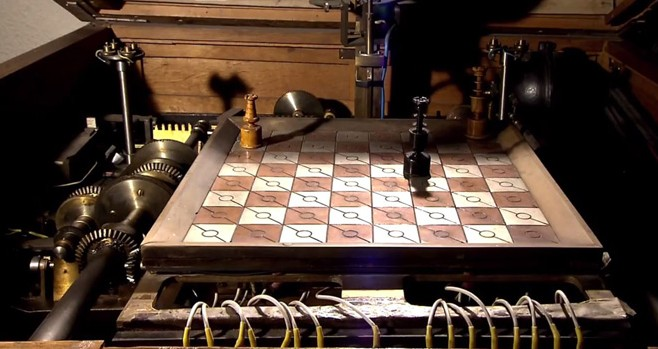
\includegraphics[width=10cm]{figs/c1/ajedrecista.jpg}
  \end{center}
  \caption[El Ajedrecista]{El Ajedrecista. Imagen obtenida de \cite{ajedrecista}}
  \label{fig:ajedrecista}
\end{figure}

En la segunda mitad del siglo XX, con el gran avanze de los ordenadores, se empiezan a ver los primeros robots tal y como se conocen hoy en día.
De esta época debemos destacar al robot industrial que desarrolló la compañía Unimate en 1952, al igual que el robot Shakey, un pequeño robot que apareció
en 1972 capaz de navegar y evitar obstáculos en una habitación cerrada sin interacción humana.

\begin{figure} [H]
  \begin{center}
    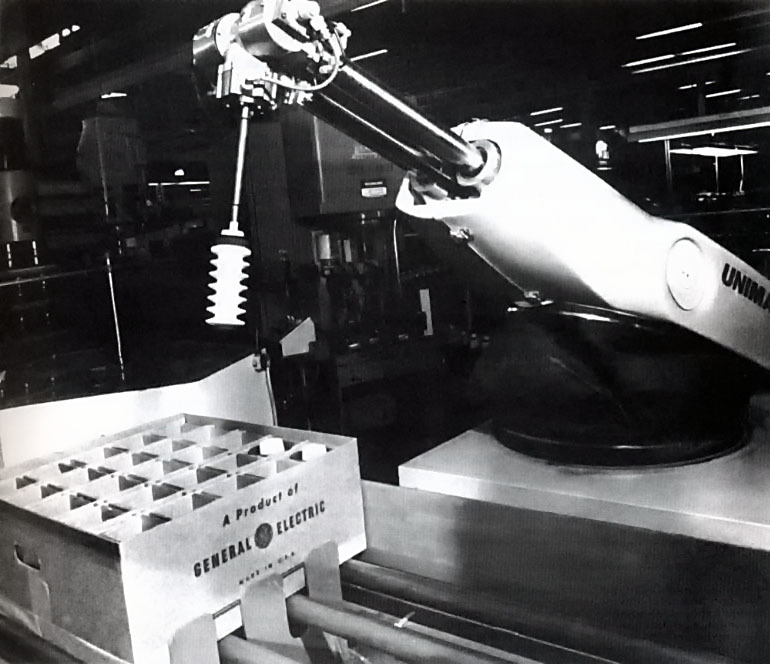
\includegraphics[width=10cm]{figs/c1/unimate.jpg}
    \includegraphics[width=5cm]{figs/c1/shakey.jpg}
  \end{center}
  \caption[Robots Unimate y Shakey]{Robots Unimate y Shakey. Imágenes obtenidas respectivamente de \cite{unimate} y \cite{shakey}}
  \label{fig:unimate_shakey}
\end{figure}

En el 2000, Honda presenta su robot ASIMO (\textit{Advanced Step in Innovative Mobility}), un humanoide que demostró un gran avance en técnicas
complejas como caminar y correr a velocidades de hasta 9km/h.\\

A partir de él surgieron varios robots humanoides con nuevas tecnologías,
como \textit{QRIO} de \textit{Sony} en 2004 siendo capaz de reconocer caras, el pequeño robot \textit{Nao} en 2008 con su habilidad para
interactuar con el ser humano o \textit{Pepper}, un robot con forma humana pero que se desplaza con ruedas que apareció en 2014 y que se usaba sobre todo
como guía o recepcionista, hasta que su desarrollo y producción se abandonó en 2021.

\begin{figure} [H]
  \begin{center}
    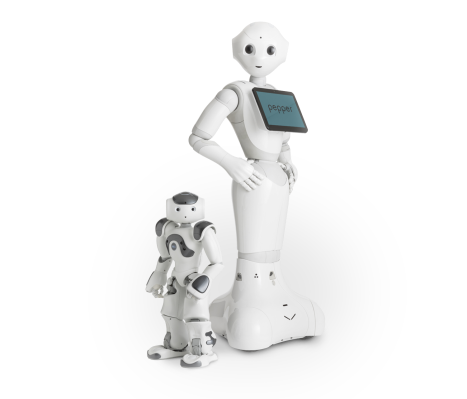
\includegraphics[width=10cm]{figs/c1/nao-pepper.png}
  \end{center}
  \caption[Robots Nao y Pepper]{Robots Nao y Pepper. Imagen obtenida de \cite{nao_pepper}}
  \label{fig:nao_pepper}
\end{figure}

Parejo a estos robots, la NASA estaba desarrollando sus propios robots para mandar a Marte. El \textit{MARS-ROVER}, una plataforma móvil con un brazo mecánico,
sensores de proximidad, láser y cámaras, salió a la luz ya en los años 70. Finalmente su sucesor, el \textit{Sojourner Rover} fue el primero en aterrizar en el
planeta rojo en 1997. En 2004, se lanzaron el \textit{Spirit} y el \textit{Oportunity} con el objetivo de encontrar evidencia de agua, contando con muchos
más sensores e instrumentos científicos que sus predecesores. Las últimas misiones, \textit{Curiosity} y el \textit{Perseverance}, que aterrizaron en
2012 y 2021 respectivamente, tenían el objetivo de buscar indicios de vida en Marte, tanto pasada como presente, a la vez que comprobar si la el desarrollo
de vida humana sería posible.

\begin{figure} [H]
  \begin{center}
    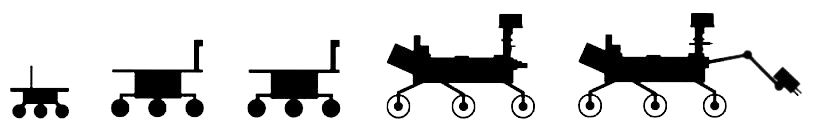
\includegraphics[width=10cm]{figs/c1/rovers.png}
  \end{center}
  \caption[Robots Mars Rovers]{Robots Mars Rovers.}
  \label{fig:rovers_mars}
\end{figure}

Hoy en día, el avance de la robótica ha llegado a una gran variedad de aplicaciones distintas. Entre ellas, podríamos destacar las aplicaciones domésticas
con robots de limpieza como los famosos \textit{Roomba} o iRobot, el sector de la agricultura con vehículos autónomos y monitorizacion de cultivos,
en logística tanto para organizar las mercancías dentro de almacenes como para el reparto, e incluso para conducción autónoma con empresas como Tesla o
Google desarrollando sus propios vehículos que son capaces de conducir grandes distancias sin interacción humana.

\begin{figure} [H]
  \begin{center}
    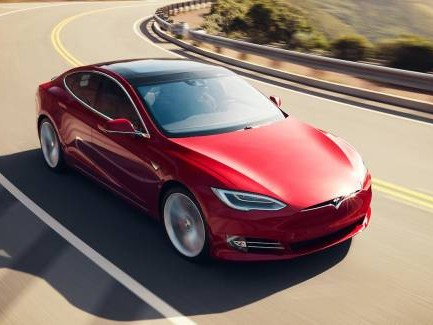
\includegraphics[width=7cm]{figs/c1/tesla-model-s-5_750x.jpg}
    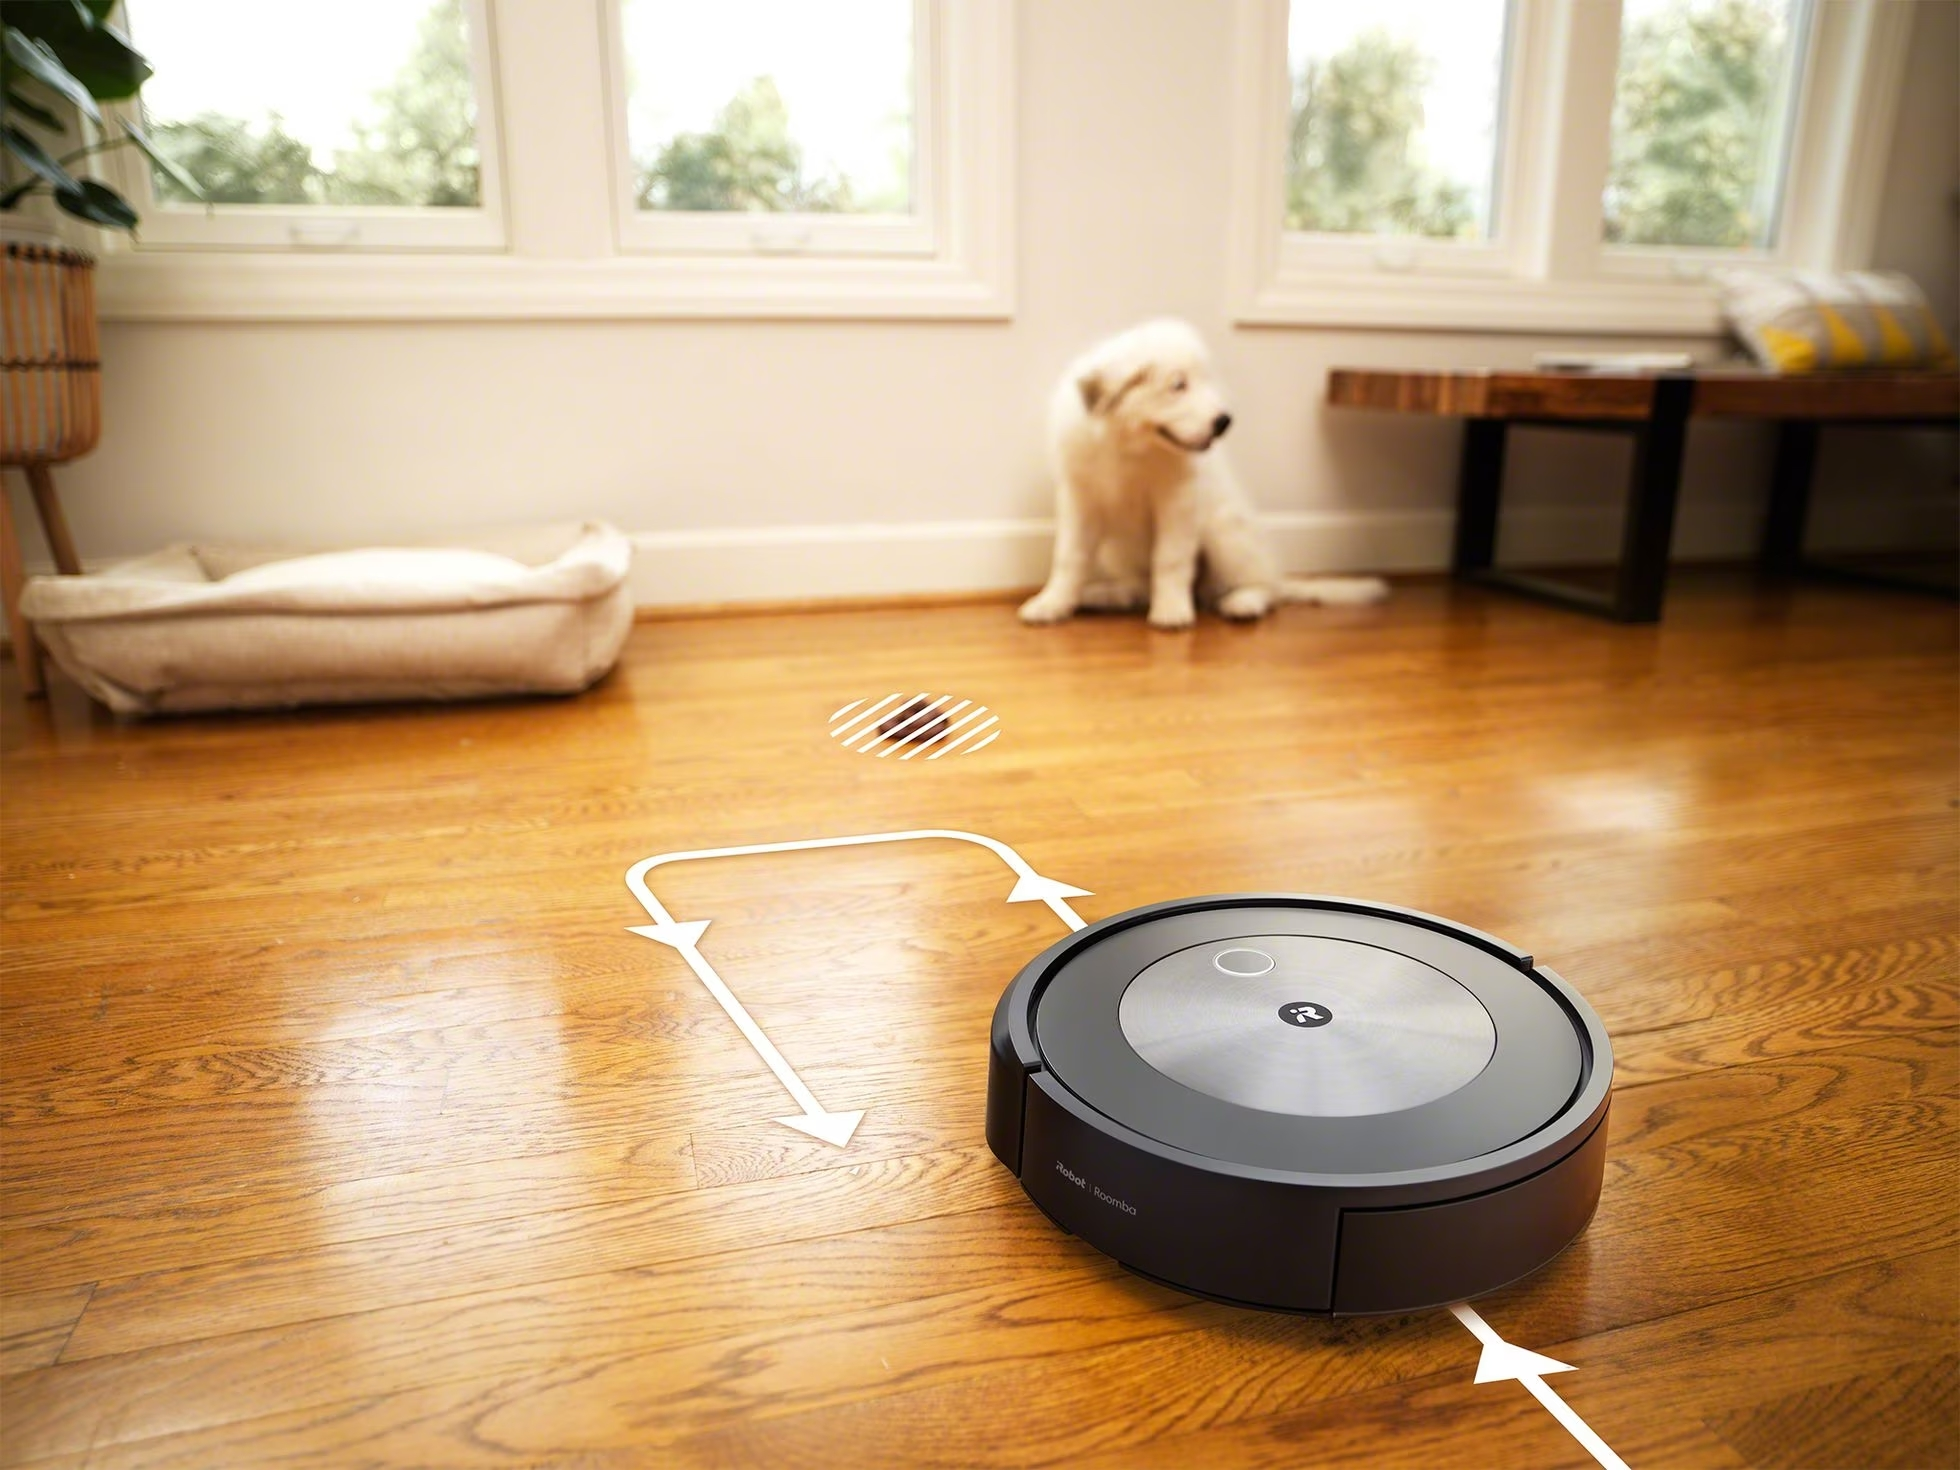
\includegraphics[width=7cm]{figs/c1/roomba.jpg}
    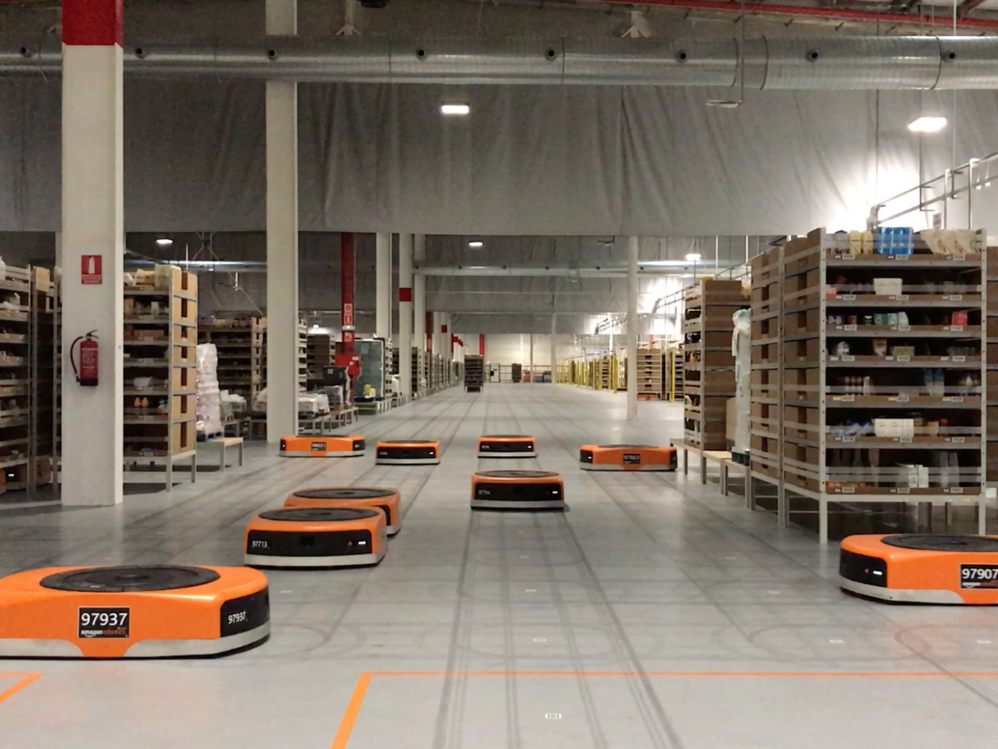
\includegraphics[width=7cm]{figs/c1/almacen.png}
    \includegraphics[width=7cm]{figs/c1/prime.jpg}
  \end{center}
  \caption[Ejemplos aplicaciones actuales robótica]{Ejemplos de aplicaciones actuales de la robótica.}
  \label{fig:rob_varios}
\end{figure}

\subsection{Educación en Robótica}
\label{subsec:urjc}

Actualmente la robótica es un mercado en alza, lo que hace que la cantidad de expertos en el sector sea escasa. 

Los conocimientos de programación es algo que, hasta hace poco, se consideraba algo de nicho y que sólo se enseñaba en algunas universidades, haciendo que
su avance y desarrollo sea lento. Hoy en día se considera algo tan fundamental, que incluso en algunas escuelas primarias se comienzan a desarrollar los
conocimientos en torno a la programación y la robótica con niños de 5 años en las aulas y en talleres.\\

El gran avance en la robótica ha causado una gran demanda de profesionales y, gracias a ello, han surgido grados universitarios como el grado en
Ingeniería de Robótica Software, impartido por la Universidad Rey Juan Carlos en el campus de Fuenlabrada.
Como indica su nombre, este grado está orientado mayoritariamente a la programación, con lenguajes como \textit{python}, \textit{C++} o
\textit{Java}, y abordando temas como inteligencia artificial, ciberseguridad o visión artificial entre otros, todo esto sin dejar de lado
el apartado físico de la robótica, con asignaturas como sensores y actuadores o mecatrónica, donde se enseña a crear robots desde cero.\\

Este grado también da acceso a los estudiantes al laboratorio de
robótica\footnote{\textbf{Laboratorio de robótica}: \url{https://labs.eif.urjc.es/index.php/laboratorios/edificio-laboratorio-iii/laboratorios-laboratorio-l3104/}},
donde podrán programar usando robots reales como el robot Pepper o el TurtleBot2\ref{sec:turtlebot2} usado en este trabajo.

\begin{figure} [H]
  \begin{center}
    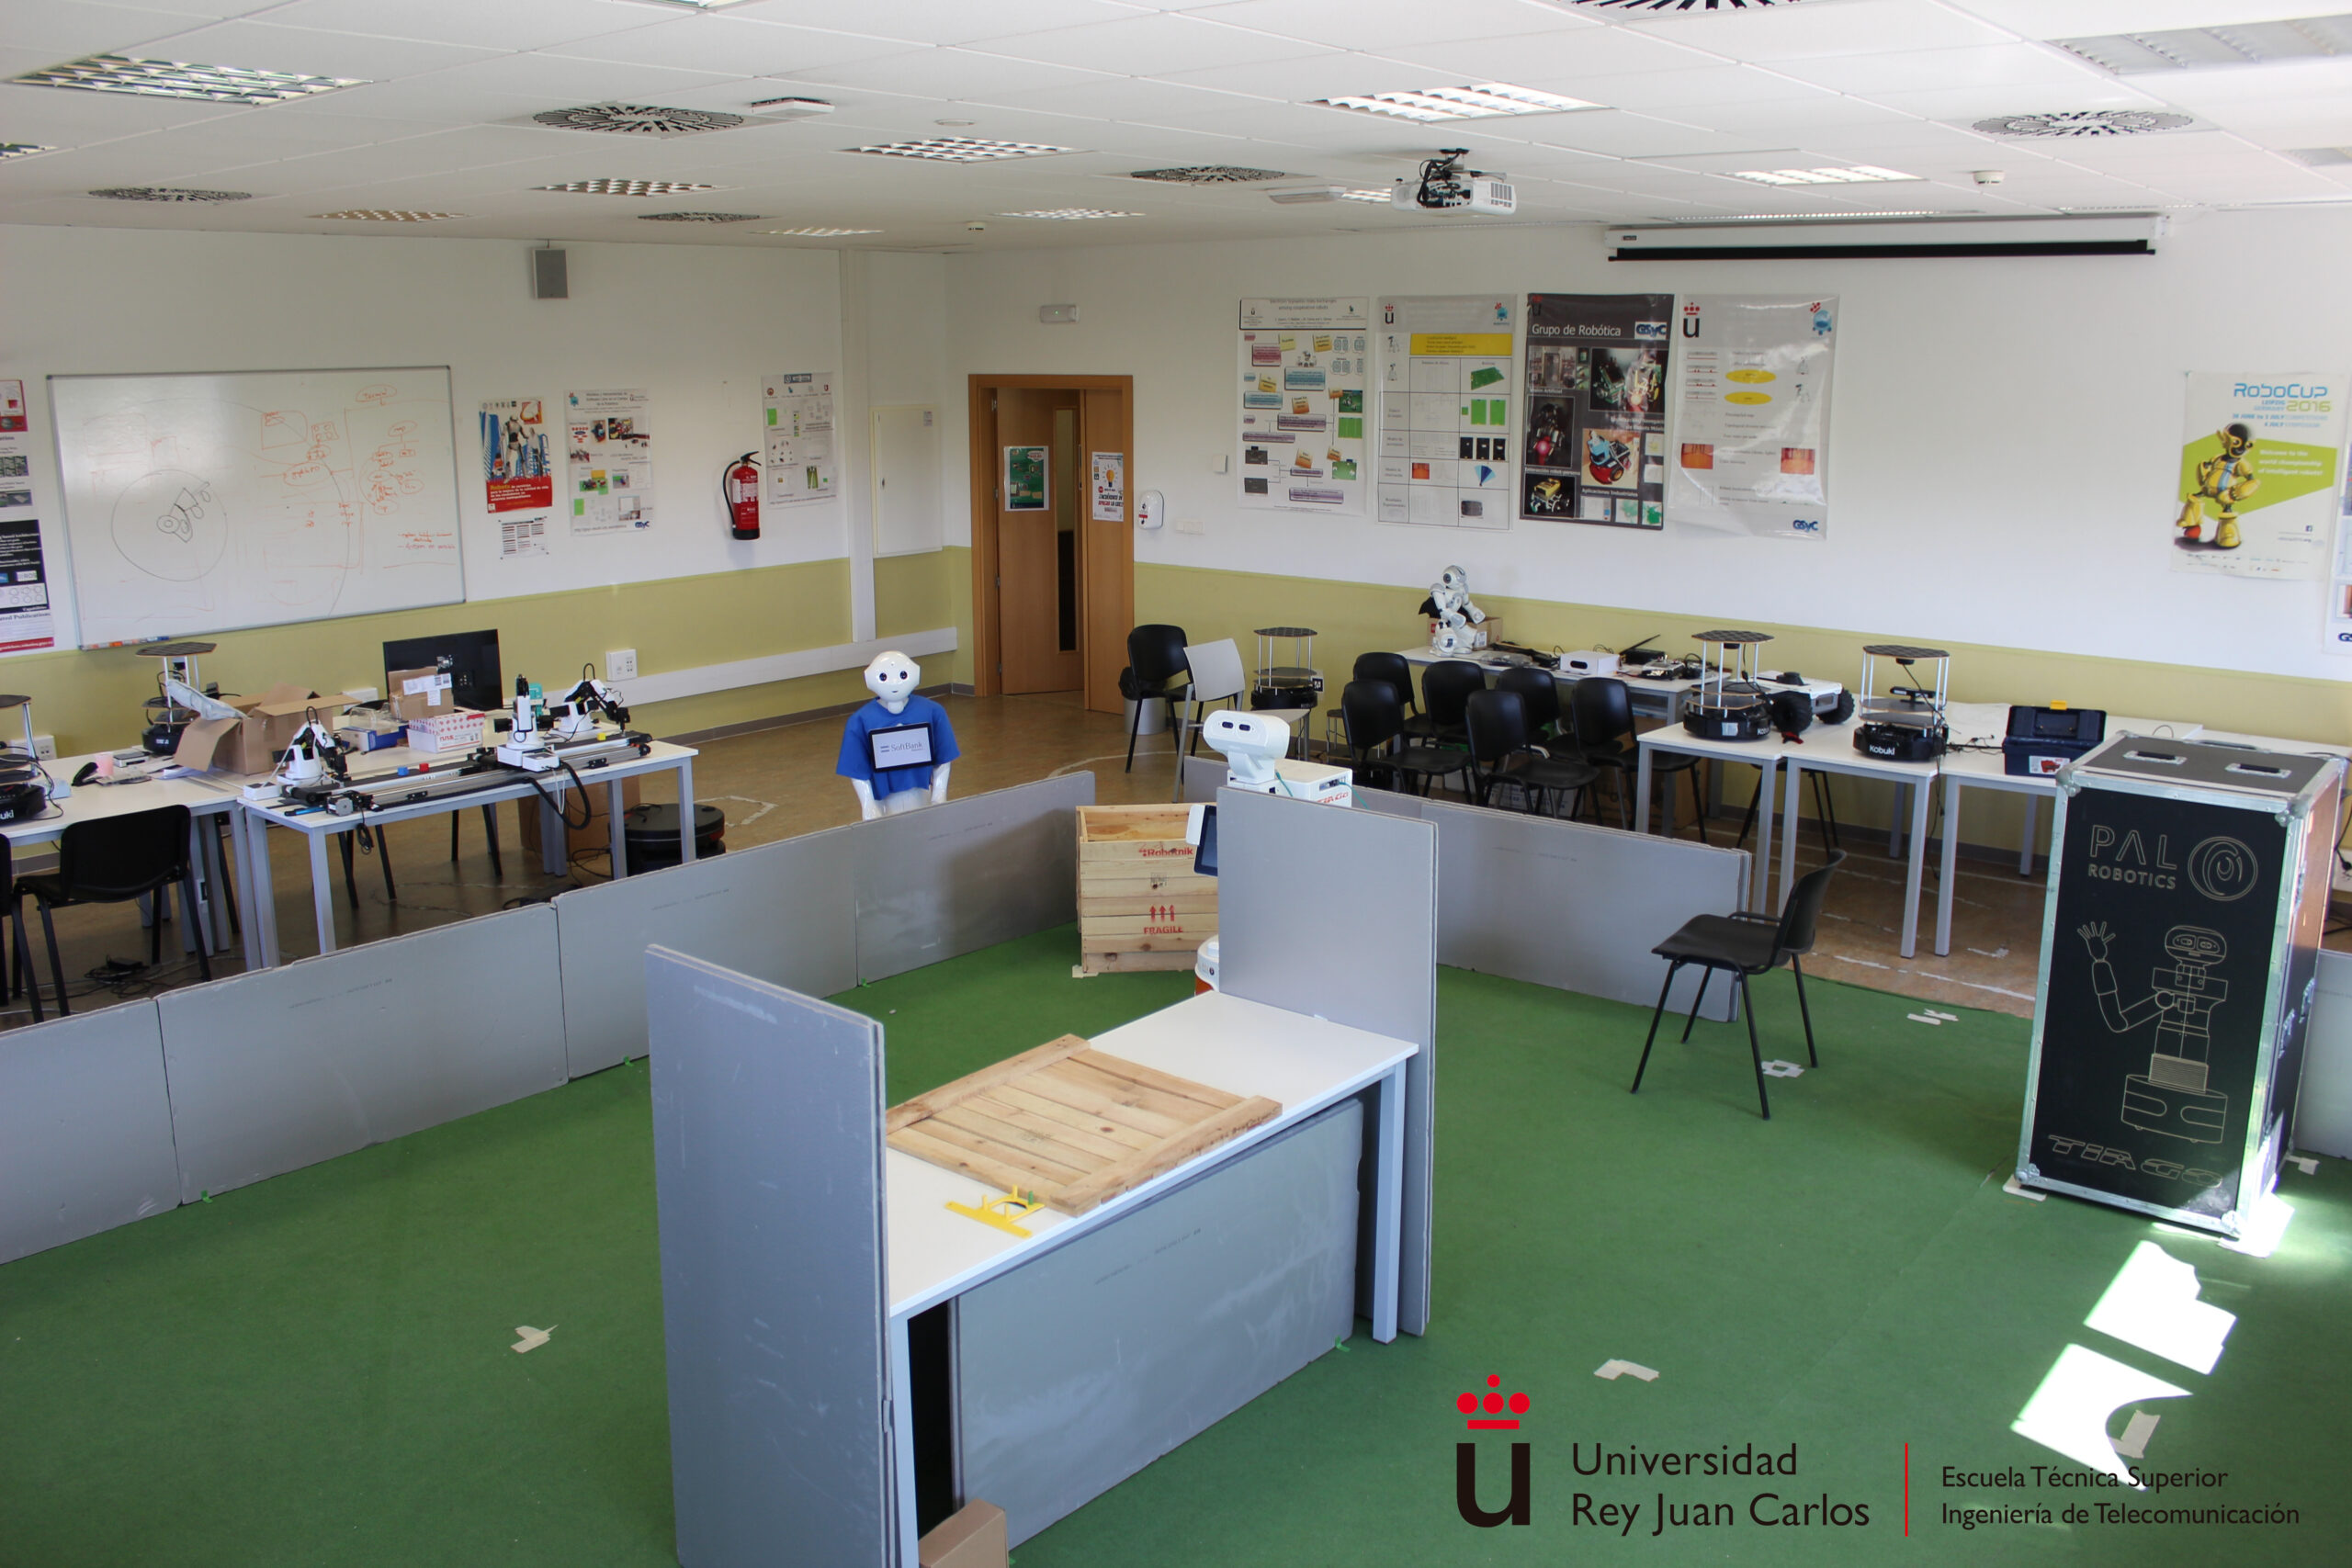
\includegraphics[width=10cm]{figs/c1/rob_lab.jpg}
  \end{center}
  \caption[Laboratorio Robótica]{Laboratorio de Robótica ETSIT.}
  \label{fig:rob_lab}
\end{figure}

\section{Programación de robots}
\label{sec:prog_rob}

El \textit{software} de los robots ha ganado cada vez más importancia a medida que las tareas a realizar se vuelven más complejas.
Gran parte del avance en la robótica se debe a las herramientas que facilitan el desarrollo de este software, como el \textit{middleware} robótico.
El \textit{middleware} más extendido en el mundo de la robótica es ROS (\ref{sec:ros2}). Este nos ofrece una gran variedad de herramientas, desde 
abstracción del hardware, hasta comunicación entre distintas partes del robot. Para usar ROS, lo más común es usar lenguajes de programación como
\textit{python3} o \textit{C++}, aunque ésta no es la única forma de programar robots.

\subsection{Lenguajes de programación visuales}
\label{subsec:vis_prog}

Un lenguaje de programación visual es aquel que permite a los usuarios crear software mediante elementos gráficos y no únicamente mediante texto,
como ocurre con los lenguajes de programación tradicional.

Un gran ejemplo de este tipo de programación es \textit{Scratch}\footnote{\textbf{Scratch}: \url{https://scratch.mit.edu/}}.
Esta plataforma nos permite programar el comportamiento de imágenes conocidas como \textit{sprites} mediante el uso de bloques simples para crear
historias interactivas, animaciones o incluso juegos, permitiendo a los usuarios compartir sus creaciones e investigar cómo lo hacen otros.
Esta plataforma es muy usada en entornos académicos (primaria y secundaria) como introducción a la programación por su simpleza a la hora de entender
conceptos básicos como bucles o condicionales. 

\begin{figure} [H]
  \begin{center}
    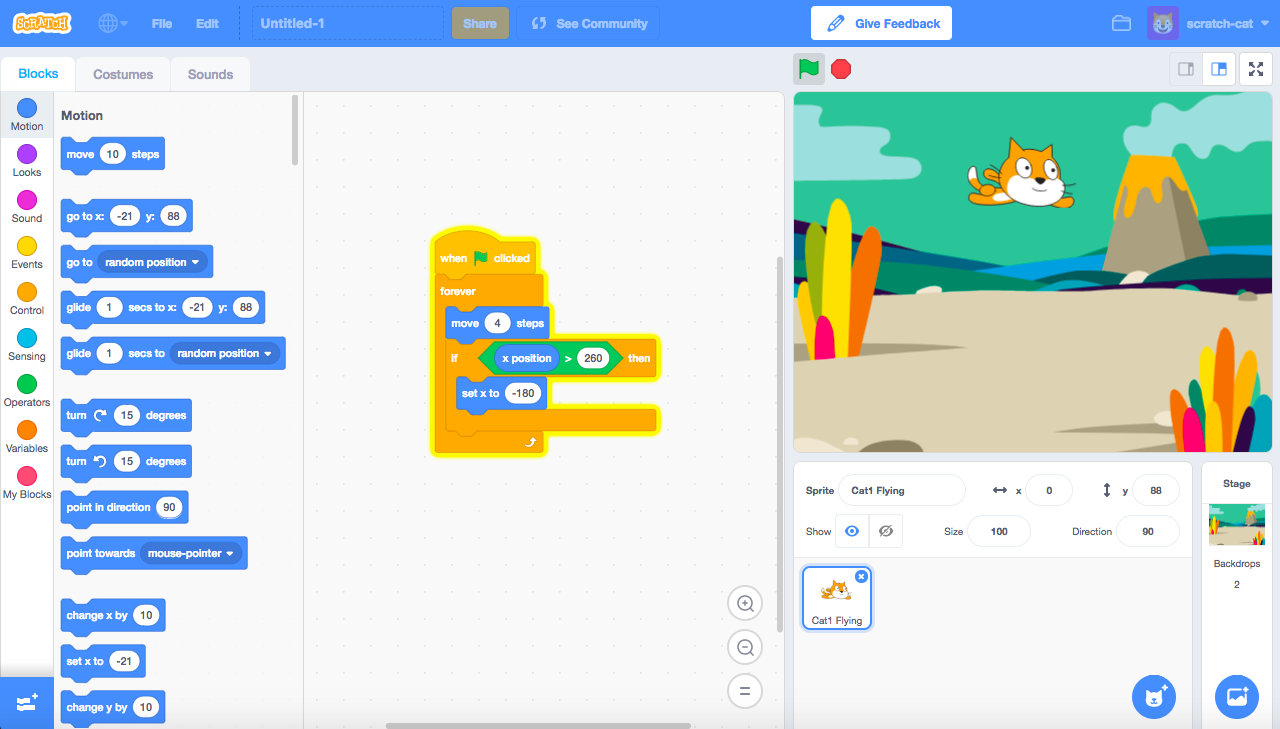
\includegraphics[width=12cm]{figs/c1/scratch.png}
  \end{center}
  \caption[Scratch]{Plataforma Scratch.}
  \label{fig:scratch}
\end{figure}

VisualCircuit, la plataforma en la que se basa este Trabajo Fin de Grado, también utiliza la programación visual mediante el uso de bloques que se
pueden colocar y unir mediante cables para crear circuitos complejos.
Estos cables envían información entre bloques, desde simples mensajes de texto hasta imágenes o matrices de valores.
La componente visual permite entender el funcionamiento del software sin necesidad de ver cada bloque por dentro.
VisualCircuit nos permite crear aplicaciones robóticas de manera rápida y sencilla sin necesidad de tener grandes conocimientos de programación
o robótica gracias a las librerías de bloques prefabricados que ofrece, destacando bloques de sensores y actuadores (láser, cámara, motores...) o bloques
de edición de imágenes.

\begin{figure} [H]
  \begin{center}
    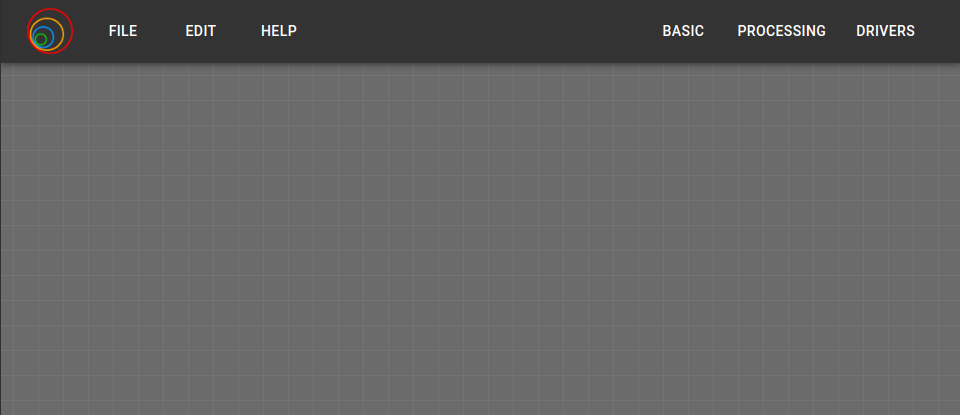
\includegraphics[width=12cm]{figs/c1/empty_VC.png}
  \end{center}
  \caption[Plataforma VisualCircuit]{Plataforma VisualCircuit.}
  \label{fig:VC_plat}
\end{figure}

En el apartado \ref{sec:visualcircuit} se profundizará en el funcionamiento de esta plataforma.

\chapter{Objetivos y metodología de Trabajo}
\label{cap:capitulo2}

\section{Objetivos}
\label{sec:objetivos}

En la herramienta VisualCircuit, antes de realizar este proyecto, ya existían bloques dedicados específicamente a la robótica para algunos sensores
(cámara, odometría e IMU\footnote{\textbf{IMU}: Inertial Measurement Unit}) y para los motores usando ROS
\textit{Noetic}\footnote{\textbf{ROS Noetic}: \url{http://wiki.ros.org/noetic}}, pero al tratarse de una versión obsoleta del middleware,
decidimos que era momento de actualizar a ROS2 \textit{Humble}\footnote{\textbf{ROS Humble}: \url{https://docs.ros.org/en/humble/index.html}},
ya que es la versión estable más moderna en el momento de realización de este Trabajo Fin de Grado.\\

Los objetivos concretos de este Trabajo Fin de Grado son los siguientes:

\begin{itemize}
	\item   Desarrollar bloques para sensores y actuadores usando ROS2 \textit{Humble} y probar su correcto funcionamiento mediante
                        circuitos simples de VisualCircuit.
                    Profundizaremos más en el capítulo \ref{cap:capitulo4}.
	\item   Diseñar y construir aplicaciones complejas que usen estos bloques para comprobar su funcionalidad en situaciones reales:
    \begin{itemize}
        \item   Aplicación sigue-persona: usar reconocimiento visual para seguir a una persona tanto en entorno simulado como real,
                    usando el robot TurtleBot2 (sección \ref{sec:turtlebot2}).
                    Veremos más en el capítulo \ref{cap:capitulo5}.
        \item   Aplicación \textit{Virtual Force Field}: usar el láser y la odometría para navegar por el entorno evitando obstáculos.
                    Examinaremos con mayor detalle en el capítulo \ref{cap:capitulo6}.
    \end{itemize}
\end{itemize}

\newpage

\section{Metodología}
\label{sec:metod}

Este Trabajo Fin de Grado comenzó en abril de 2022 y finalizó en junio de 2023. Durante estos meses se ha seguido el siguiente modelo de trabajo: 

\begin{itemize}
	\item   Reuniones cada dos semanas con el tutor del TFG para analizar los avances, recibir retroalimentación y buscar soluciones en caso
                de bloqueo.
	\item   Uso de un blog\footnote{\textbf{Blog}: \url{https://roboticslaburjc.github.io/2022-tfg-david-tapiador/}} donde se iba actualizando el
                progreso antes de las reuniones, donde se puede comprobar el desarrollo cronológico del trabajo.
	\item   Todo el material usado y desarrollado durante este Trabajo Fin de Grado se ha ido actualizando en un repositorio público de
                GitHub\footnote{\textbf{GitHub del TFG}: \url{https://github.com/RoboticsLabURJC/2022-tfg-david-tapiador}}.
\end{itemize}

\section{Plan de Trabajo}
\label{sec:work_plan}

Como se ha dicho en el anterior punto, el desarrollo de este TFG ha durado algo más de un año. Este periodo se ha dividido en varias etapas: 

\begin{enumerate}
	\item   \textbf{Pruebas con VisualCircuit}: Realizar circuitos para entender el funcionamiento de la plataforma, desarrollando bloques
                propios que modifiquen imágenes o compartan información.
	\item   \textbf{Inicio del TFG}: Configuración del entorno de pruebas (instalación de ROS2 \textit{Humble}, diseño de mundos
                en \textit{Gazebo}...)..
    \item   \textbf{Desarrollo de bloques drivers con ROS2}: Actualización y creación de bloques para sensores y actuadores usando ROS2 \textit{Humble}.
    \item   \textbf{Prueba de los bloques en situaciones reales}: Desarrollo de aplicaciones robóticas avanzadas para probar el correcto
                funcionamiento de los bloques implementados. 
    \item   \textbf{Memoria del Trabajo Fin de Grado}: Redacción de esta memoria. 
\end{enumerate}



\chapter{Herramientas y plataforma de desarrollo}
\label{cap:capitulo3}

El desarrollo de nuevo contenido para la plataforma de VisualCircuit, ha necesitado usar distintas herramientas, como por ejemplo programación, ROS2, gazebo..., por lo que voy a hacer una pequeña descripción de cada una, así como el uso que se le ha dado dentro del proyecto.

\section{Lenguaje de programación}
\label{sec:lenguaje_programación}
% ** LENGUAJES DE PROGRAMACÍON
% ** PYTHON

Python es un lenguaje interpretado de alto nivel. Este lenguaje busca facilitar la legibilidad del código, convirtiéndolo en uno de los más comunes a día de hoy. Es un lenguaje de programación multiparadigma, ya que soporta tanto programación orientada a objetos, como programación imperativa y funcional.\\

\begin{code}[H]
    \begin{lstlisting}[language=python]
    print("Hello World")
    \end{lstlisting}
    \caption[Hola mundo en python]{Hola mundo en python}
    \label{cod:holamundo_python}
\end{code}

Dentro del TFG se usará para la programación dentro de la plataforma VisualCircuit (\ref{sec:visualcircuit}).

\section{ROS2 (Robot Operating System 2)}
\label{sec:ros2}
% ** MIDDLEWARE ROS2

ROS\footnote{\textbf{ROS}: \url{http://wiki.ros.org/es}} o Robot Operating System es un \textit{middleware}\footnote{{\textbf{Middleware}: software que se sitúa entre las aplicaciones y el sistema operativo}} formado por un conjunto de herramientas y librerías de software libre empleadas para el desarrollo de aplicaciones robóticas. Su objetivo es ofrecer una plataforma estándar para todas las ramas de la robótica.\\

ROS se basa en una arquitectura \textit{cliente-servidor} centralizado que, mediante suscriptores y publicadores, permite enviar información, ya sean medidas de sensores, cambios de estado, decisiones usando árboles de decisión, órdenes a los actuadores, etc.\\

Para comunicarse con los servidores (o como se llaman en ROS, \textit{topics}) se usan nodos. Estos nodos pueden contar con varios publicadores y suscriptores simultáneaos.
Cada \textit{topic} se define con un tipo de mensaje, que será el único que se pueda enviar y recibir a través de él. Estos tipos de mensajes pueden ser mensajes simples como una cadena de caracteres o tipos compuestos con otros tipos, permitiéndonos crear topics adecuados a las necesidades de cada proyecto.\\

\begin{figure} [H]
    \begin{center}
        \includegraphics[width=7cm]{figs/c3/ros_comunicación.png}
    \end{center}
    \caption[Comunicación del nodo Master con los nodos Intermedios y con distintos sensores y actuadores.]{Comunicación del nodo Master con los nodos Intermedios y con distintos sensores y actuadores. Imagen obtenida de \cite{comunicacion_ros2}}
    \label{fig:ros_master_comunicacion}
\end{figure}

ROS2 lo usaremos para obtener información del robot turtlebot2 (\ref{sec:turtlebot2}), tanto real como simulado, como por ejemplo su posición en el entrono simulado o las últimas medidas de sus sensores, y para comandarle instrucciones (velocidades a sus motores)

\section{Gazebo}
\label{sec:gazebo}
% ** GAZEBO

Gazebo\footnote{\textbf{Gazebo}: \url{https://classic.gazebosim.org/}} es un simulador 3D de código abierto orientado a la robótica que permite fusionar escenarios realistas con robots simulados, ofreciendo un entorno seguro para probar algoritmos. Éste utiliza el motor de físicas ODE\footnote{\textbf{Open Dynamics Engine}: \url{https://www.ode.org/}}, aunque se puede configurar con otros motores, como Bullet\footnote{\textbf{Bullet}: \url{https://pybullet.org/wordpress/}} o DART\footnote{\textbf{DART}: \url{https://dartsim.github.io/}}.\\

Al estar orientado a la robótica, permite integrar fácilmente modelos de robots reales con sensores (incluso simulando sus ruidos) y enviar a través de los distintos topics de ROS o ROS2 (\ref{sec:ros2}) alguna información directa del simulador, como la posición, medidas de los sensores simulados o incluso información de objetos no programables (del entorno).

\begin{figure} [H]
    \begin{center}
        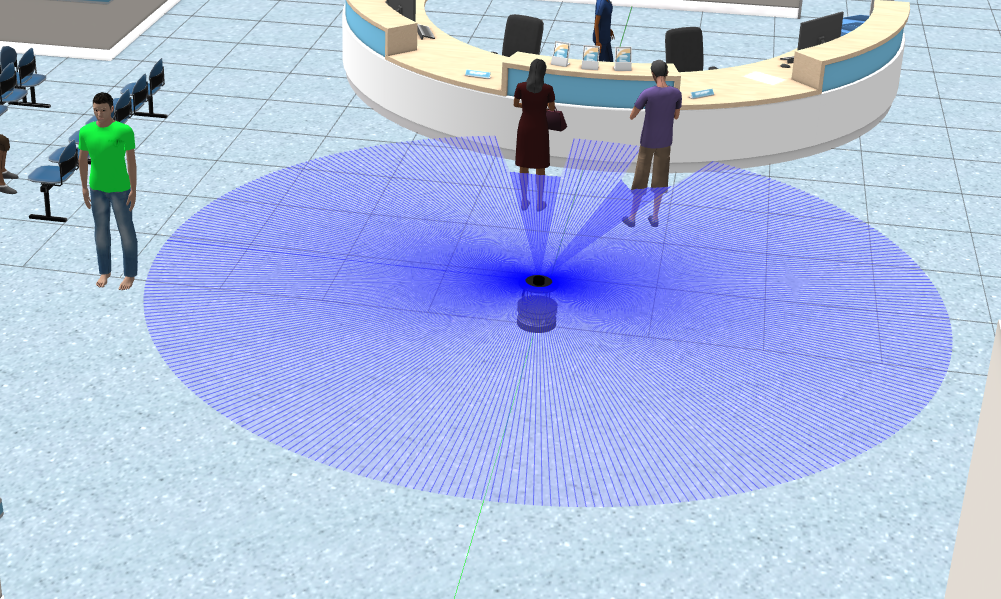
\includegraphics[width=7cm]{figs/c3/gazebo_sim.png}
    \end{center}
    \caption[Simulador Gazebo.]{Ejemplo de ejecución en gazebo.}
    \label{fig:gazebo_example}
\end{figure}

A lo largo de todo el proyecto, usaremos gazebo para simular el turtlebot2 (\ref{sec:turtlebot2}) al igual que los distintos entornos que iremos usando para probar los programas.
 
\section{Turtlebot2}
\label{sec:turtlebot2}
% ** TURTLEBOT2

La URJC de Fuenlabrada, en sus laboratorios de robótica, cuenta con varios robots Turtlebot2\footnote{\textbf{Turtlebot2}: \url{https://www.turtlebot.com/turtlebot2/}} a disposición de los alumnos del grado. Estos son perfectos para la enseñanza e investigación en robótica, por su sencilla introducción a temas como ROS o el uso de sensores. Los Turtlebot2 están formados por dos partes principales: una base Kobuki y una estructura superior.


\subsection{Base Kobuki}
\label{subsec:turtlebot2_base}
% ** TURTLEBOT2 -> KOBUKI

La base del Turtlebot2 se llama \textit{Kobuki}. En apariencia, es similar a un robot de limpieza como podrían ser los Roomba. En cuanto al hardware, lleva integrados tres bumpers (sensores de contacto), odometría, sensor de caída y varios giroscopios. Tiene una velocidad lineal máxima de 0.7 m/s y angular de 180 grados/s. Su batería le permite una autonomía de entre 3 y 7 horas. Cuenta con varios puertos, entre ellos un USB para poder conectar nuestro portatil y ejecutar los distintos algoritmos.\\

Algunos de los paquetes de ROS2 que instalaremos para poder usarlo son los drivers del kobuki para ROS2-Humble\footnote{\textbf{Drivers kobuki ROS2-Humble}: \url{https://github.com/IntelligentRoboticsLabs/Robots/tree/humble/kobuki}} de IntelligentRoboticsLabs, compañeros de la URJC. Siguiendo las instrucciones de instalación que se encuentran en dicho repositorio de github, accedemos a varios paquetes básicos para el uso de kobuki, como \textit{kobuki\_ros} o \textit{kobuki\_node}, entre otros.

\begin{figure} [H]
    \begin{center}
        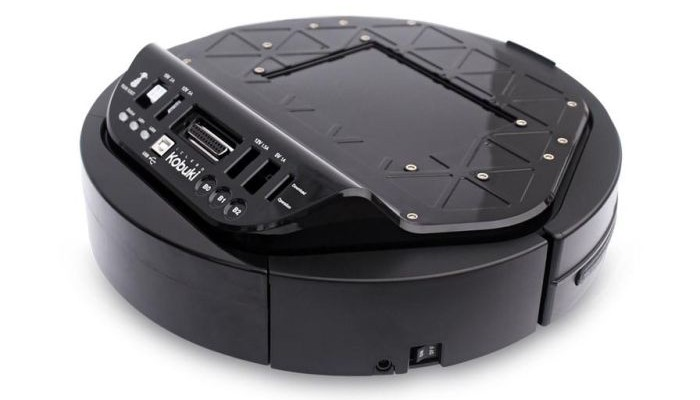
\includegraphics[width=7cm]{figs/c3/kobuki_base.jpg}
    \end{center}
    \caption[Kobuki base]{Base kobuki. Imagen obtenida de \cite{kobuki_base}}
    \label{fig:kobuki_base}
\end{figure}

\subsection{Cuerpo Turtlebot2}
\label{subsec:turtlebot2_body}
% ** TURTLEBOT2 -> CUERPO
El cuerpo del turtlebot2 (también conocido como \textit{TurtleBot Structure}) está formado por una serie de plataformas y tubos que se atornillan a la base kobuki y permiten fijar nuevos sensores, como podrían ser una cámara o un láser, o actuadores como brazos robóticos. También ofrece un sitio cómodo para poder colocar el portátil encima del robot y así poder conectarlo a la base mediante USB. 


\begin{figure} [H]
    \begin{center}
        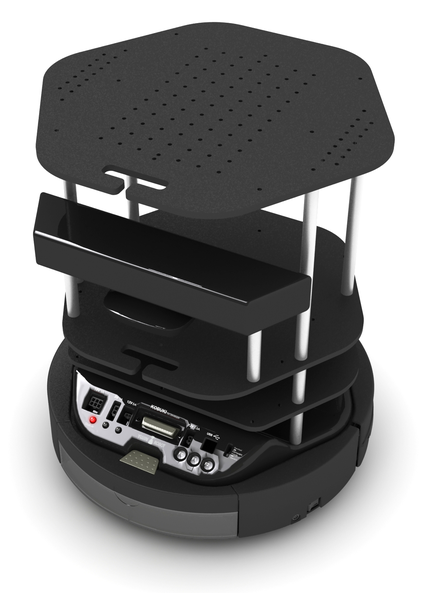
\includegraphics[width=5cm]{figs/c3/turtlebot2_body.jpg}
    \end{center}
    \caption[Turtlebot2]{Turtlebot2. Imagen obtenida de \cite{turtlebot_2_structure}}
    \label{fig:turtlebot_2_structure}
\end{figure}

\subsection{Turtlebot2 simulado}
\label{subsec:turtlebot2_sim}
% ** TURTLEBOT2 -> SIMULADOR

Para algunas partes del proyecto, como el desarrollo de drivers para ROS2 (\ref{cap:capitulo4}) o el VFF usando máquinas de estados (\ref{cap:capitulo6}), hemos usado el simulador para probar y desarrollar los algoritmos. Para esto, he tenido que usar un modelo del turtlebot2 que cuenta con los mismos sensores (cámara, RPLIDAR, bumper, etc) que el real, así como los mismos topics.\\

Para integrar el modelo del robot en el simulador, necesitamos su representación en URDF\footnote{\textbf{URDF}: Unified Robot Description Format}, una forma estandarizada de crear los modelos de los robots inluyendo sus sensores y actuadores, partes móviles etc.

\begin{figure} [H]
    \begin{center}
        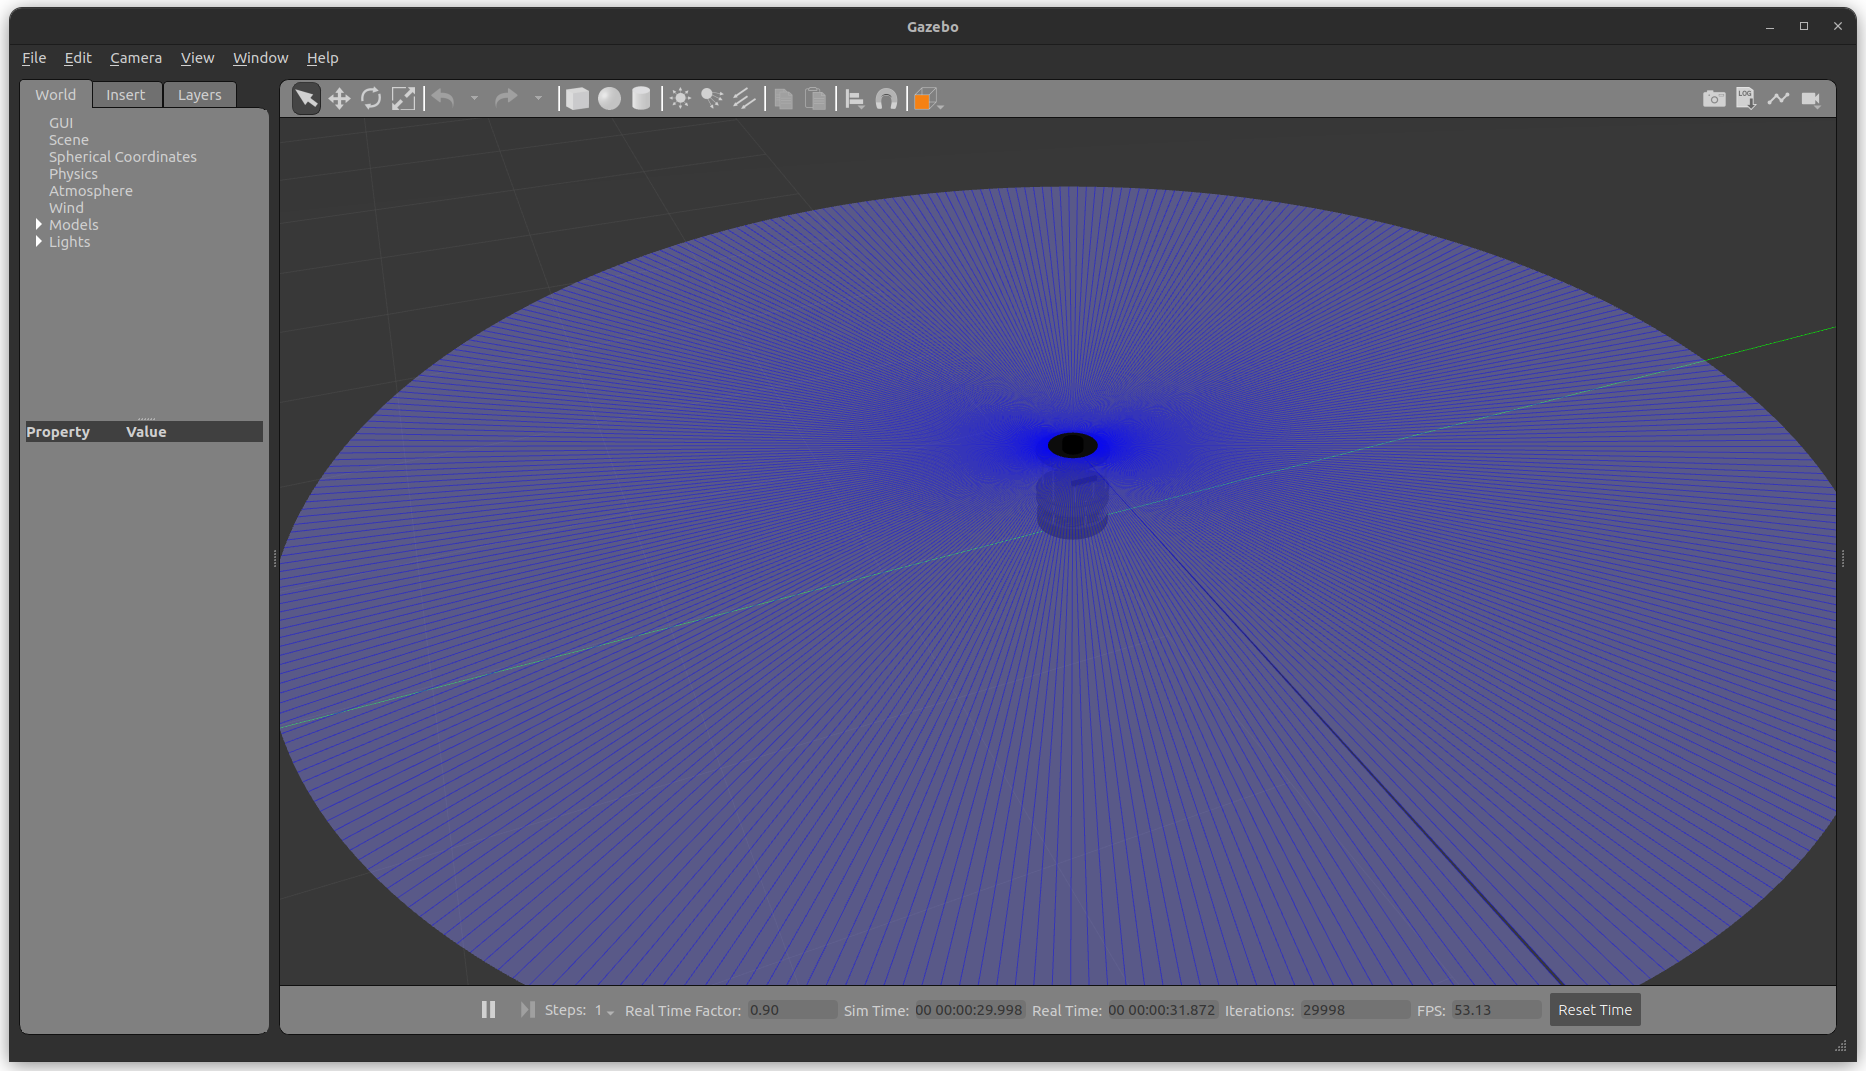
\includegraphics[width=14cm]{figs/c3/turtlebot2_sim.png}
    \end{center}
    \caption[Turtlebot2 simulado]{Turtlebot2 en gazebo.}
    \label{fig:turtlebot_2_sim}
\end{figure}


\newpage

\section{RVIZ2}
\label{sec:rviz2}
% ** RVIZ2

RVIZ2 es una herramienta de visualización 3D para robots, el ambiente y las medidas de los sensores de éstos.

\begin{figure} [H]
    \begin{center}
        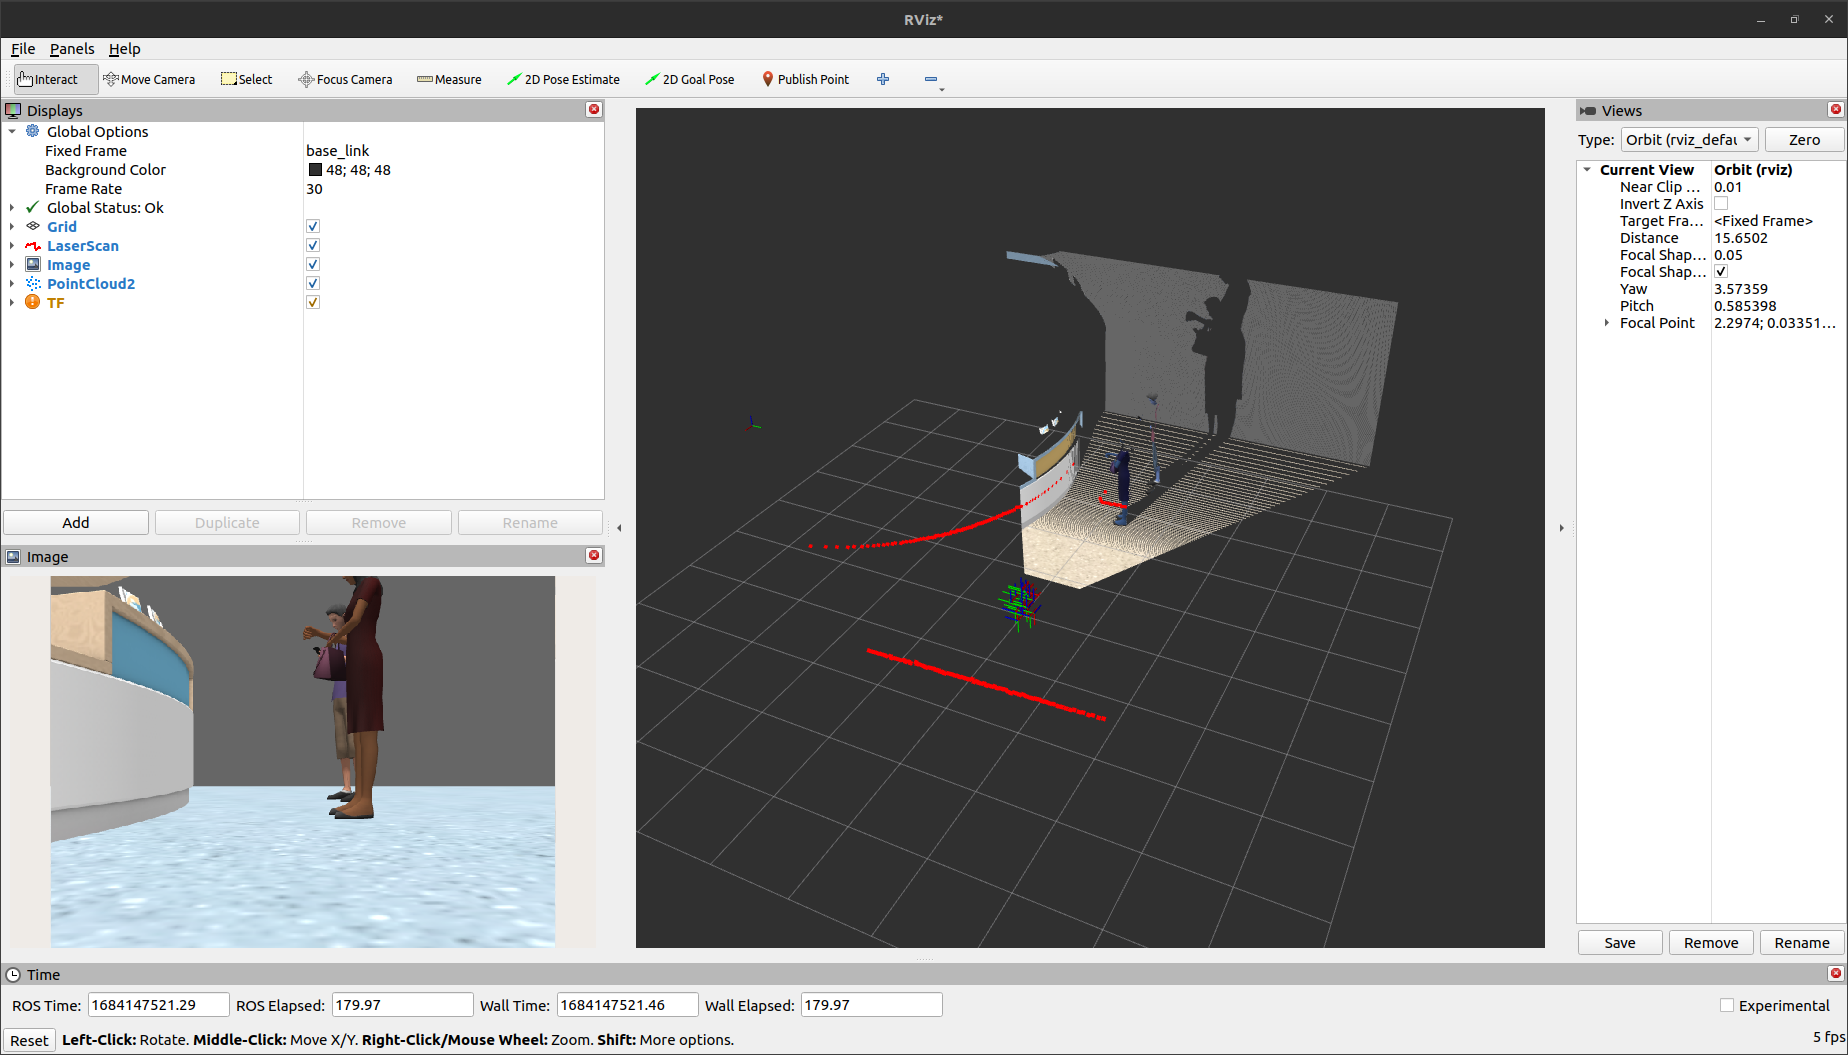
\includegraphics[width=13cm]{figs/c3/RVIZ2.png}
        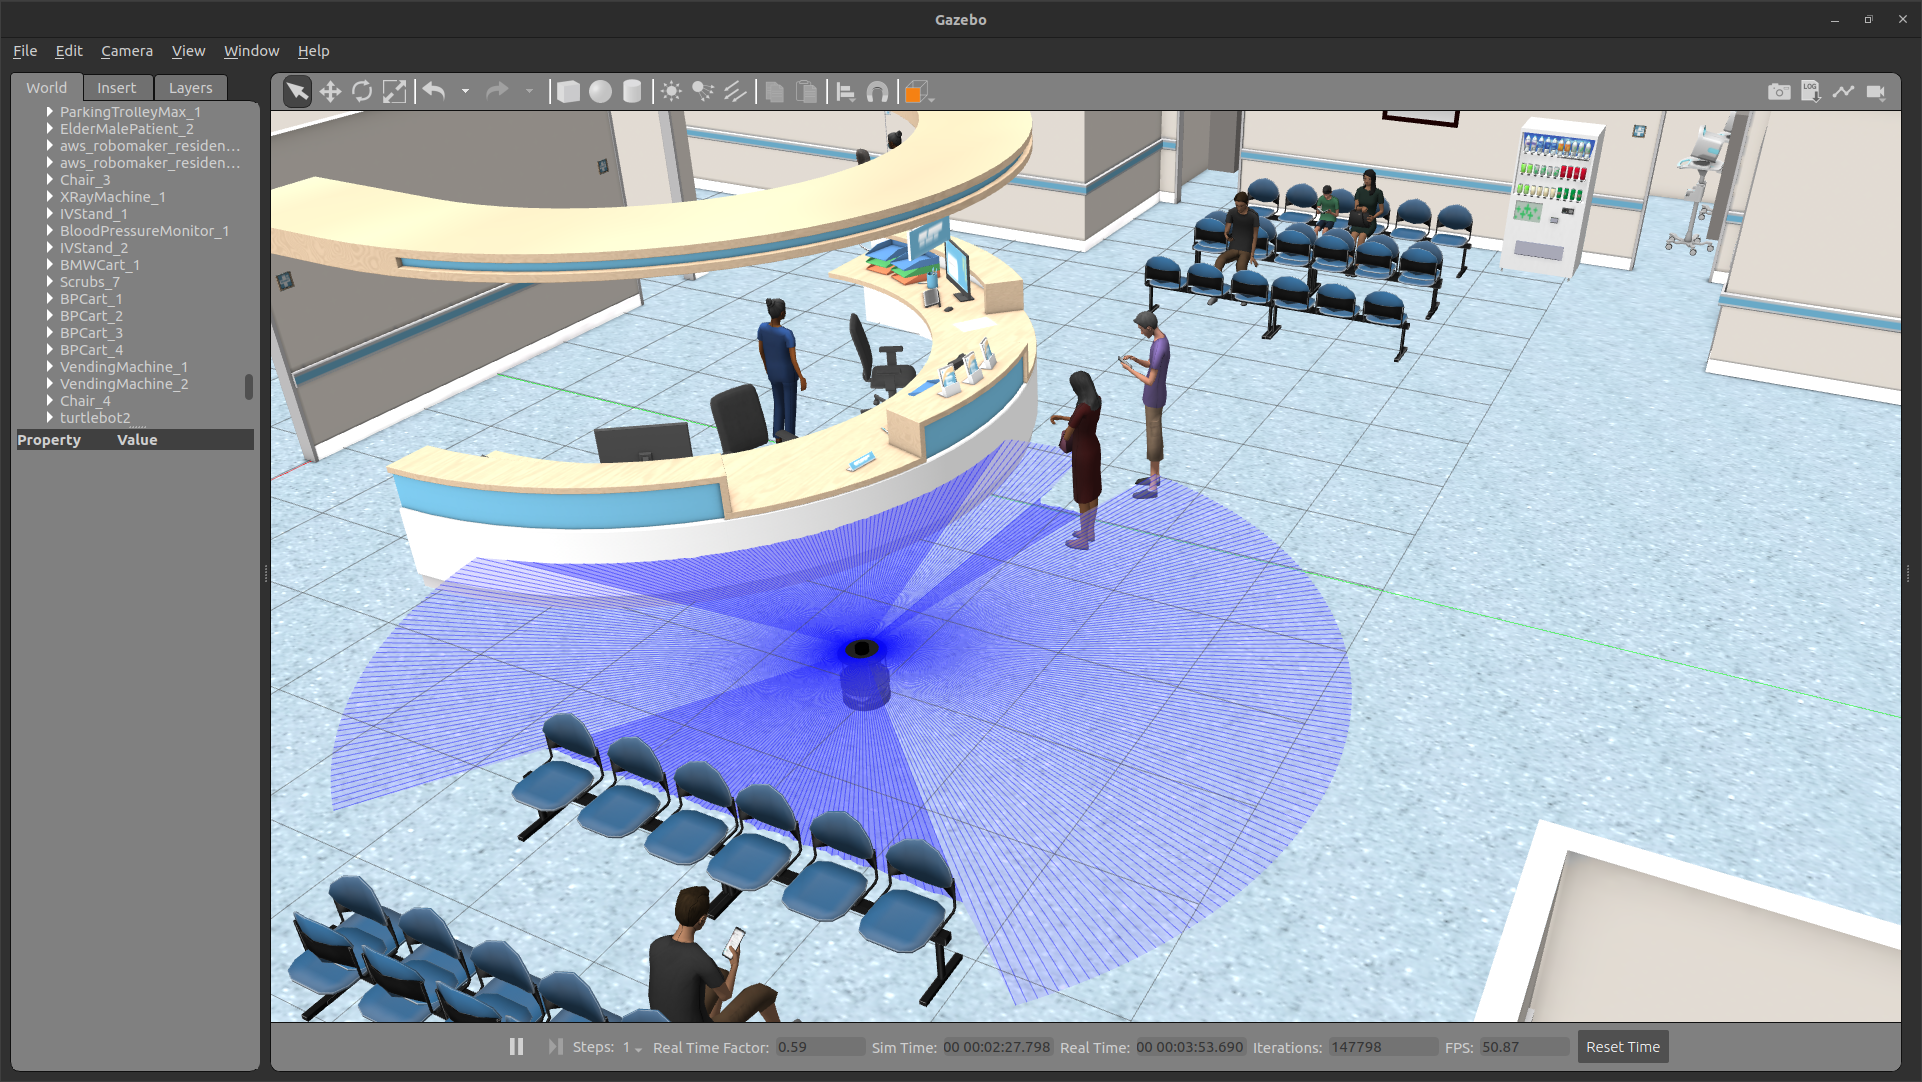
\includegraphics[width=13cm]{figs/c3/Gazebo_RVIZ.png}
    \end{center}
    \caption[RVIZ2 Vs mundo gazebo]{Ejemplo de RVIZ2 frente al mundo gazebo real.}
    \label{fig:rviz2_example}
\end{figure}

RVIZ2 se usará bastante durante el proyecto tanto para depurar como para observar las medidas de los distintos sensores a tiempo real.

\newpage

\section{Sensores}
\label{sec:sensores}
% ** SENSORES

Como hemos mencionado anteriormente, un robot se compone, a grandes rasgos, de sensores y actuadores. Para este proyecto se han usado varios de ellos, por lo que aquí hay una pequeña introducción a cada uno.

\subsection{Cámara ASUS Xtion Pro}
\label{subsec:asus_xtion}
% ** ASUS XTION
La cámara \textit{ASUS Xtion} es una cámara RGB-D\footnote{\textbf{RGB-D}: RedGreenBlue-Depth, hace referencia las cámaras que captan la imagen y las distancias de cada pixel.}, que ofrece tanto imagen como una nube de puntos con la distancia medida para cada pixel de la imagen.
Esta cámara ofrece una imágen de 720p, con una frecuencia de 60fps. En la parte de profundidad, es capaz de captar desde 0.8m hasya 3.5 con un ángulo efectivo de 70º. Se conecta mediante USB directamente al ordenador.\\
En el proyecto, como debemos usarla con ROS2, usaremos el paquete creado por un usuario de internet\footnote{\textbf{Drivers ASUS-Xtion ROS2}: \url{https://github.com/mgonzs13/ros2_asus_xtion}}.\\
\begin{figure} [H]
    \begin{center}
        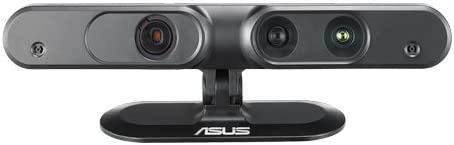
\includegraphics[width=5cm]{figs/c3/asus_xtion.jpg}
    \end{center}
    \caption[Cámara ASUS-XTION]{Cámara ASUS-XTION. Imagen obtenida de \cite{asus_xtion}}
    \label{fig:asus_xtion}
\end{figure}



\subsection{RPLIDAR A2}
\label{subsec:rplidar_a2}
% ** RPLIDAR

Se trata de un láser de 360º con un rango de medida desde 0.2m hasta 16m y una frecuencia de muestreo que se puede ajustar desde 5Hz hasta 15Hz. Usando los drivers mencionados en el apartado del Turtlebot2 (\ref{subsec:turtlebot2_base}) encontraremos un paquete para poder activar y usar este sensor con ROS2.\\

\begin{figure} [H]
    \begin{center}
        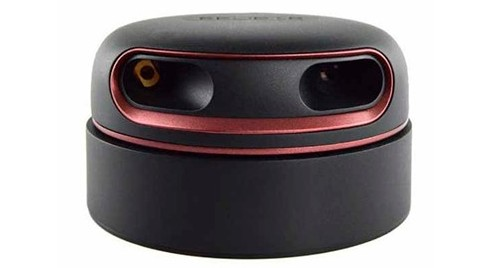
\includegraphics[width=5cm]{figs/c3/rplidar-a2.jpg}
    \end{center}
    \caption[RPLIDAR A2]{Sensor RPLIDAR A2. Imagen obtenida de \cite{rplidar}}
    \label{fig:rplidar}
\end{figure}

\section{VisualCircuit}
\label{sec:visualcircuit}
% ** VISUALCIRCUIT

VisualCircuit\footnote{\textbf{VisualCircuit Docs}: \url{https://jderobot.github.io/VisualCircuit/}} es un editor visual online basado en programación por bloques de código orientado al desarrollo de aplicaciones robóticas. Está desarrollado sobre IceStudio\footnote{\textbf{IceStudio Project}: \url{https://github.com/FPGAwars/icestudio}}.\\

\begin{figure} [H]
    \begin{center}
        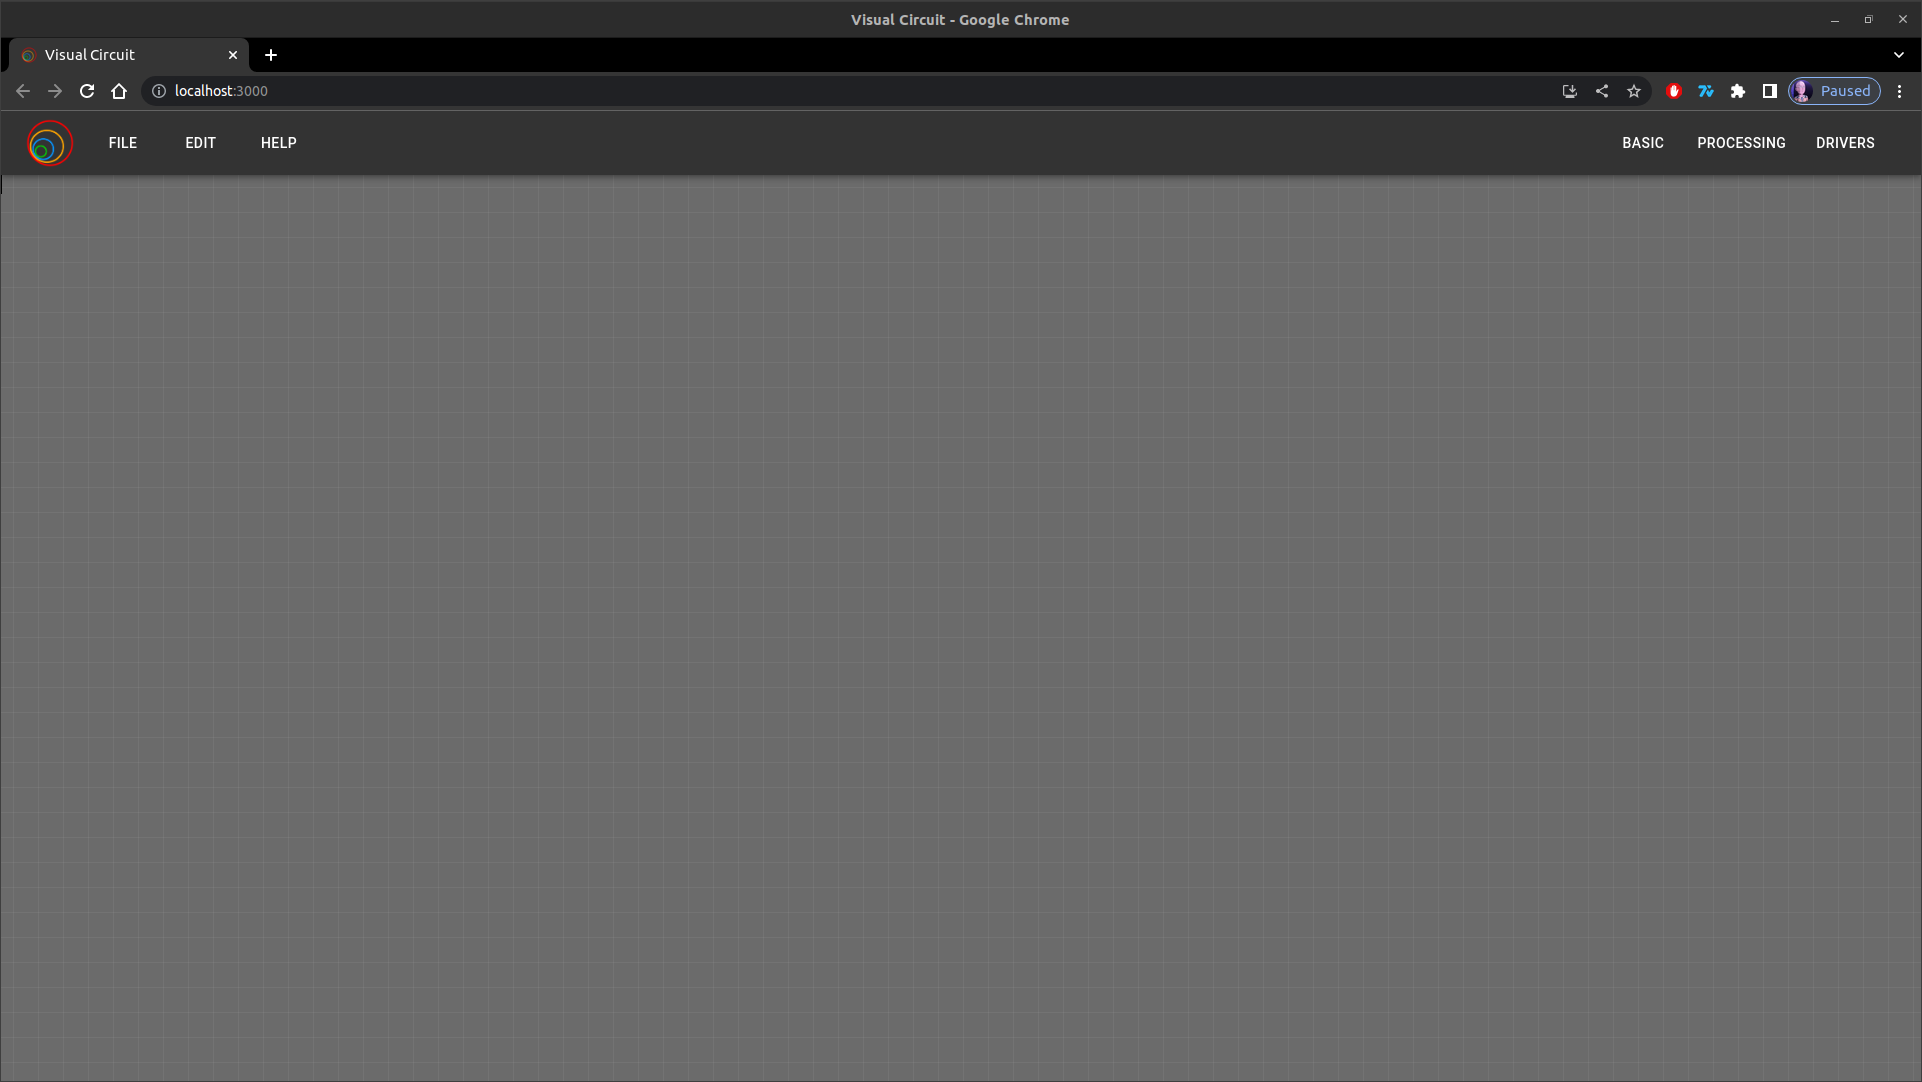
\includegraphics[width=13cm]{figs/c3/empty_VC.png}
    \end{center}
    \caption[VisualCircuit]{Página de VisualCircuit.}
    \label{fig:VC_empty}
\end{figure}

Los bloques que se pueden usar están divididos en varias pestañas: \textit{basics}, \textit{processing} y \textit{drivers}.\\
En la primera pestaña, podemos encontrar bloques simples, como inputs y outputs, bloques para definir parámetros y constantes, o bloques para insertar nuestro código.\\
En la pestaña de procesamiento, donde encontramos otros tres desplegables para bloques de control (PID), bloques relacionados con OpenCV\footnote{\textbf{OpenCV}: \url{https://opencv.org/}} y edición de imagen (filtros de color, detección de contornos, erosión, etc), y el último corresponde a \textit{TensorFlow}, que contiene un bloque para detección de objetos.\\
En la última pestaña, están los drivers que conectan con los sensores y actuadores: motor (ROS y ROS2), lector de imagenes desde archivos y desde cámaras, pantalla para mostrar las imágenes e incluso cámaras usando ROS.\\

\newpage
Ésta será la herramienta principal en torno a la que girará este proyecto, tanto buscando añadir funcionalidades como en desarrollar aplicaciones con ella.

\begin{figure} [H]
    \begin{center}
        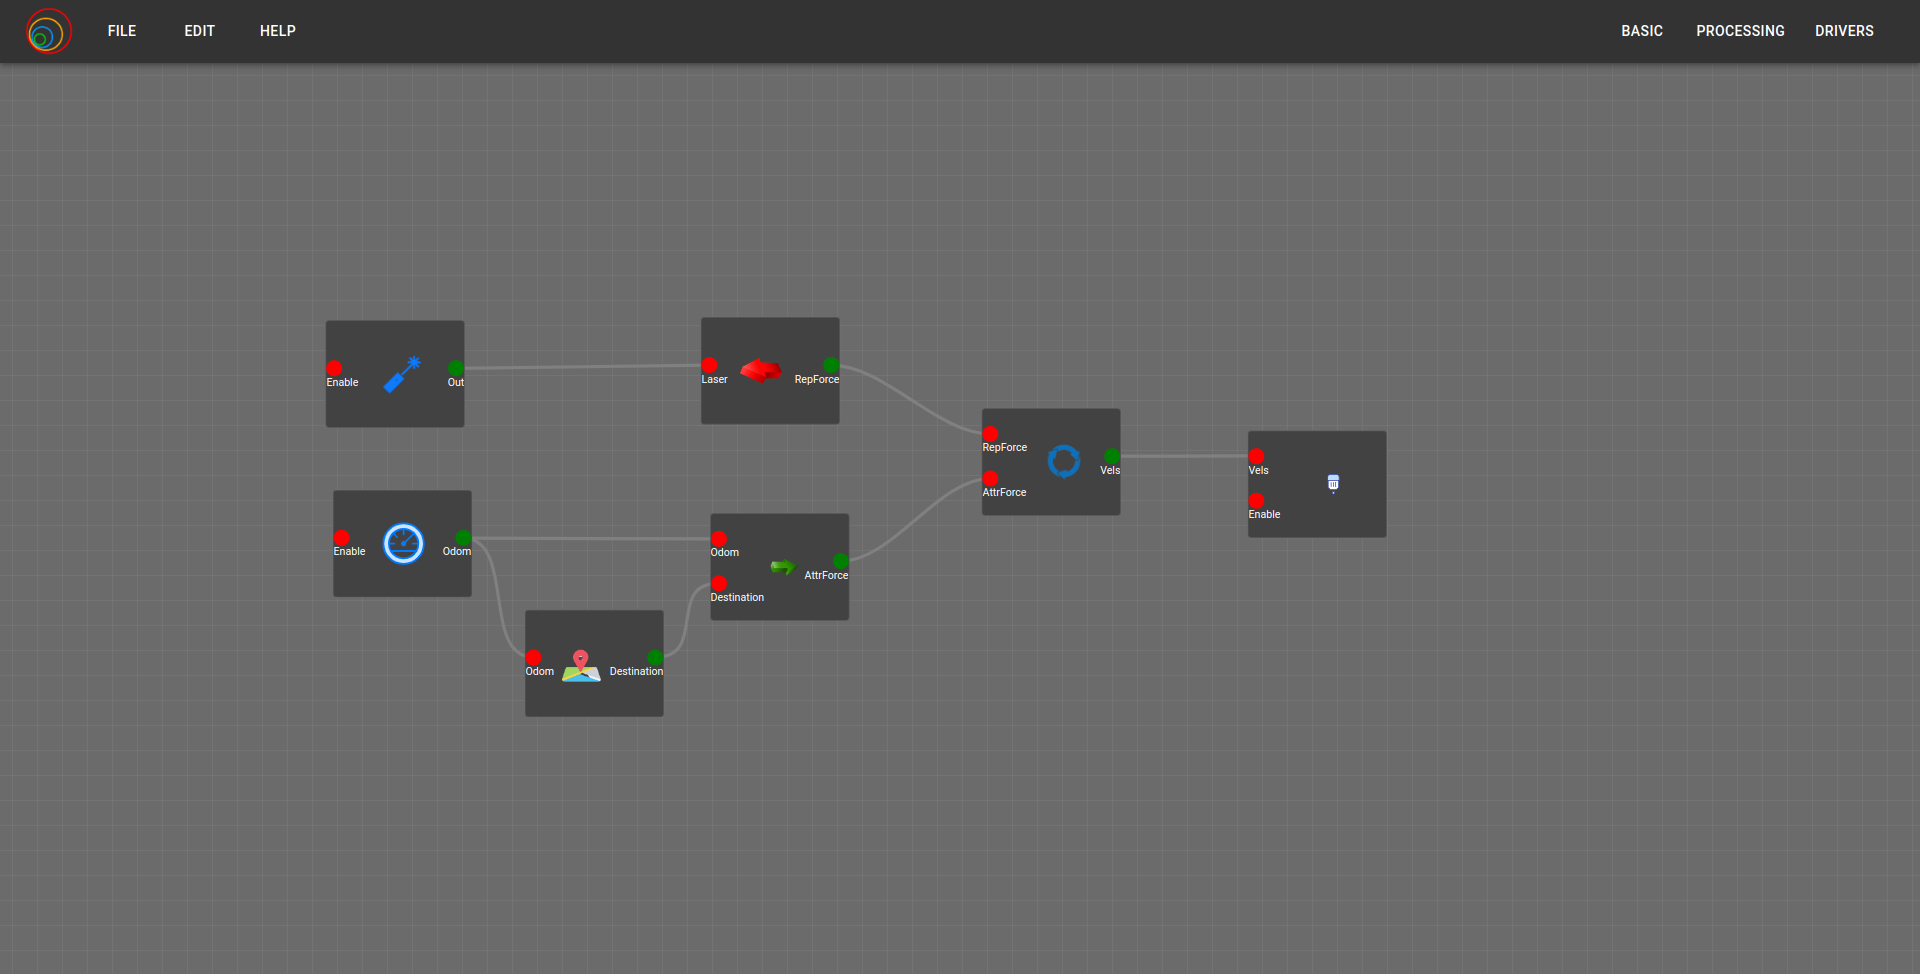
\includegraphics[width=13cm]{figs/c3/VC_example.png}
    \end{center}
    \caption[Ejemplo VisualCircuit]{Ejemplo de proyecto de VisualCircuit.}
    \label{fig:ex_VC}
\end{figure}






\chapter{Desarrollo de bloques driver}
\label{cap:capitulo4}
Como ya he explicado, VisualCircuit es una plataforma de programación online mediante el uso de bloques, pero para que esté actualizado,
hay que ir añadiendo bloques nuevos que ofrezcan esas nuevas funciones y añadirlos a las listas de bloques estándar que ofrece la página.\\
En este capítulo profundizaremos en el funcionamiento de la plataforma VisualCircuit así como en el proceso seguido para desarrollar nuevos
bloques para poder añadir ROS2 a la misma.


\section{Introducción a VisualCircuit}
\label{sec:VC_intro}

En VisualCircuit, antes de realizar este proyecto, ya existían bloques dedicados específicamente a la robótica para algunos sensores
(cámara, odometría e IMU\footnote{\textbf{IMU}: Inertial Measurement Unit}) y para los motores usando ROS
melodic\footnote{\textbf{ROS melodic}: \url{http://wiki.ros.org/melodic}}, pero al tratarse de una versión antigua, decidimos que ya era
momento de actualizar a ROS2 humble\footnote{\textbf{ROS humble}: \url{https://docs.ros.org/en/humble/index.html}}, ya que era la versión estable
más moderna hasta el momento.
\begin{figure} [H]
  \begin{center}
      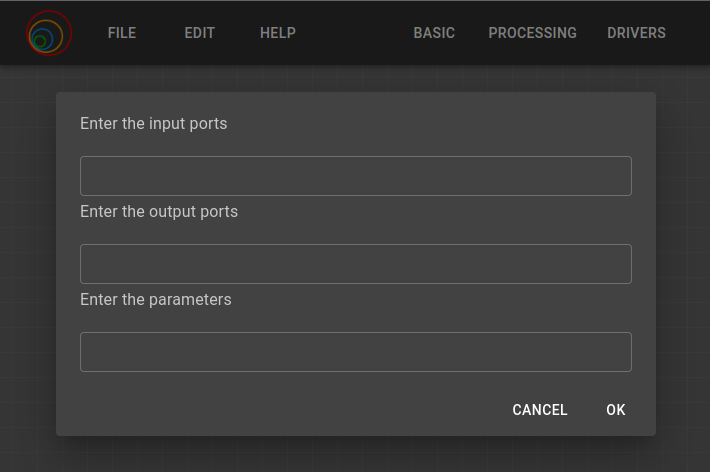
\includegraphics[width=9cm]{figs/c4/VC_pre_codeblock.png}
  \end{center}
  \caption[Creando un bloque en VisualCircuit]{Creando un bloque en VisualCircuit.}
  \label{fig:VC_creando_bloque}
\end{figure}

Para crear nuestro propio bloque, debemos añadir varios bloques prefabricados. Para introducir nuestro código principal usaremos el bloque \textit{code},
como se puede ver en la figura \ref{fig:VC_creando_bloque}. Al crearlo, se nos permite definir el número de entradas, salidas y parámetros que tendrá nuestro código.

Una vez definidos, tenemos que usar bloques de \textit{Input}, \textit{Output} y \textit{Constant} y así, usando ``\textit{Save as}'',
podemos exportarlo para usarlo como un bloque nuevo.
\begin{figure} [H]
  \begin{center}
      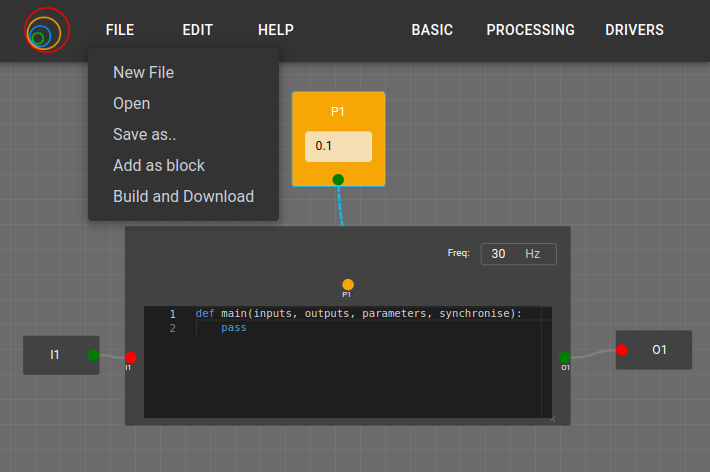
\includegraphics[width=10cm]{figs/c4/VC_saveas.png}
  \end{center}
  \caption[Guardando un bloque en VisualCircuit]{Guardando un bloque en VisualCircuit.}
  \label{fig:VC_saveas_bloque}
\end{figure}

Cuando tengamos varios bloques generados, podemos usar la opción \textit{FILE} \overrightarrow{ } \textit{Add as block} para añadir como nuevos bloques
los que acabamos de crear y así formar un circuito completo con el comportamiento que queramos.
\begin{figure} [H]
  \begin{center}
      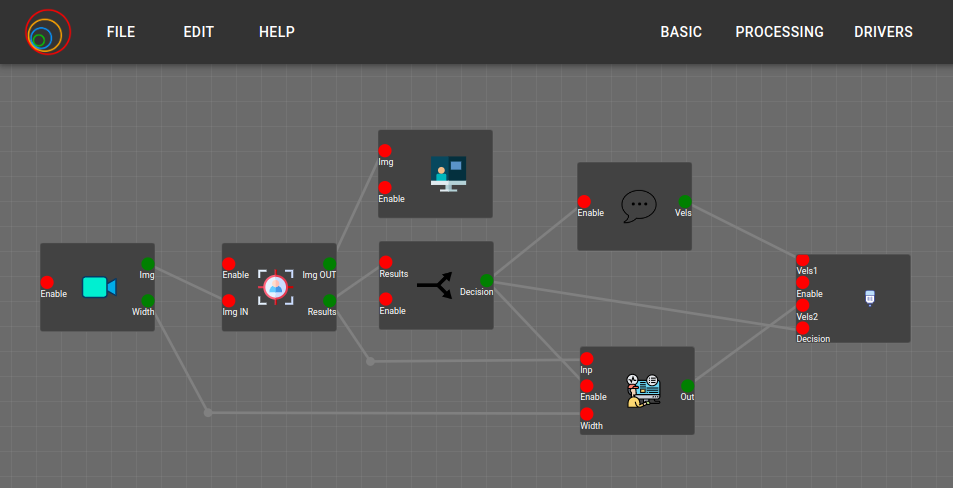
\includegraphics[width=10cm]{figs/c4/VC_example.png}
  \end{center}
  \caption[Ejemplo de proyecto en VisualCircuit]{Ejemplo de proyecto en VisualCircuit.}
  \label{fig:VC_example}
\end{figure}

Este es el funcionamiento general que debemos de seguir para usar VisualCircuit. Ahora, para crear bloques drivers nuevos para usar con ROS2
debemos centrarnos más en el código.

\section{Creación de bloques drivers}
\label{sec:drivers_creacion}

Los bloques drivers que vamos a desarrollar son para implementar la cámara, el láser y los motores usando un topic de ROS2.
Para los sensores (cámara y laser) tenemos que crear la estructura que queremos seguir, ya que ambos serán similares entre sí.\\

Usando un \textit{input} para activar/desactivar el bloque habilitaremos el uso de máquinas de estados con nuestro bloque.
También queremos compartir la medida del sensor, por lo que añadimos un \textit{output}. Por último, usamos una constante donde definiremos
el \textit{topic} del que obtendremos las lecturas del sensor. Esto lo hacemos para que el usuario no tenga que cambiar el código del bloque para cambiar
el \textit{topic} del que obtiene la información.\\
\begin{figure} [H]
  \begin{center}
      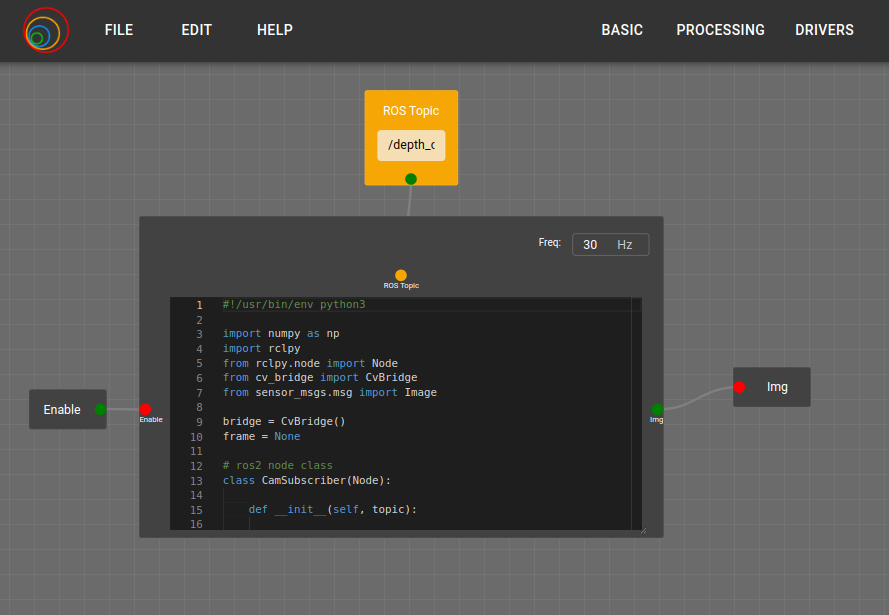
\includegraphics[width=10cm]{figs/c4/VC_driver_blocks.png}
  \end{center}
  \caption[Modelo bloque driver sensores]{Modelo para crear bloques driver de sensores.}
  \label{fig:VC_driver_model}
\end{figure}

En cuanto al código que usaremos, seguiremos las indicaciones de los manuales de
ROS2-humble\footnote{\url{https://docs.ros.org/en/humble/Tutorials/Beginner-Client-Libraries/Writing-A-Simple-Py-Publisher-And-Subscriber.html\#write-the-subscriber-node}}
para usar nodos suscriptores/publicadores con python. El código general para los bloques de sensores (suscriptores) será el siguiente:

\begin{code}[H]
  \begin{lstlisting}[language=python]
    import numpy as np
    import rclpy
    from rclpy.node import Node
    from cv_bridge import CvBridge
    from std_msgs/msg import String #SENSOR MSG TYPE
    
    bridge = CvBridge()
    data = None
    
    # ros2 node class
    class SENSORSubscriber(Node):
        def __init__(self, topic):
            super().__init__('sensor_subscriber')
            self.subscription = self.create_subscription(
              String, topic, self.callback, 10)

            self.subscription  # prevent unused variable warning
    
        def callback(self, msg):
            global data
            # Modify msg as needed and save into global variable
            data = msg

    def main(inputs, outputs, parameters, synchronise):
        global data
        auto_enable = False
        try:
            enable = inputs.read_number('Enable')
        except Exception:
            auto_enable = True
        rclpy.init()
        sensor_sub = SENSORSubscriber(parameters.read_string("ROSTopic"))

        try:
            while auto_enable or inputs.read_number('Enable'):
                data =  None
                rclpy.spin_once(sensor_sub)
                if data is not None:
                    outputs.share_string("Output", data)
                synchronise()
        except Exception as e:
            print('Error:', e)
            pass
        finally:
            print("Exiting")
            synchronise()     
            SENSORSubscriber.destroy_node()
            rclpy.shutdown()
  \end{lstlisting}
  \caption[Modelo de código para bloques drivers]{Modelo de código para bloques drivers.}
  \label{cod:bloques_drivers_sensors_total}
\end{code}

Si lo analizamos por partes, la clase \textbf{\textit{SENSORSubscriber}} (código \ref{cod:bloques_drivers_sensors_node_class}) contiene una función
para inicializar la clase, donde se define el nombre del nodo, se crea el suscriptor y se inicia el suscriptor, y una función callback a la que se
llamará de forma periódica, actualizando el valor de la variable global a la última medida del sensor.

\begin{code}[H]
  \begin{lstlisting}[language=python]
    # ros2 node class
    class SENSORSubscriber(Node):
        def __init__(self, topic):
            super().__init__('sensor_subscriber')
            self.subscription = self.create_subscription(
              String, topic, self.callback, 10)

            self.subscription  # prevent unused variable warning
    
        def callback(self, msg):
            global data
            # Modify msg as needed and save into global variable
            data = msg
  \end{lstlisting}
  \caption[Clase del nodo suscriptor para bloques drivers]{Clase del nodo suscriptor para los bloques drivers.}
  \label{cod:bloques_drivers_sensors_node_class}
\end{code}

En la función main (código \ref{cod:bloques_drivers_sensors_main_general}) tenemos dos partes, la secuencia \textit{try-except} donde se declara
si se está usando una maquina de estados (\textit{enable}) o si debe estar activo constantemente (\textit{autoenable} al haber dado error la lectura
del cable de \textit{enable}).
En la segunda parte (bucle \textit{while}) se reinicia el valor de la variable global y se llama a \textit{``rclpy.spin\_once()"} para obtener la
última medida del sensor y compartirla por el cable \textit{``output"}.

\begin{code}[H]
  \begin{lstlisting}[language=python]
    def main(inputs, outputs, parameters, synchronise):
        global data
        auto_enable = False
        try:
            enable = inputs.read_number('Enable')
        except Exception:
            auto_enable = True
        rclpy.init()
        sensor_sub = SENSORSubscriber(parameters.read_string("ROSTopic"))

        try:
            while auto_enable or inputs.read_number('Enable'):
                data =  None
                rclpy.spin_once(sensor_sub)
                if data is not None:
                    outputs.share_string("Output", data)
  \end{lstlisting}
  \caption[Función main para bloques drivers de sensores]{Función main para los bloques drivers de sensores.}
  \label{cod:bloques_drivers_sensors_main_general}
\end{code}

Una vez que tenemos el modelo general para estos bloques, hay que modificarlos para que funcionen con la cámara y con el láser. Para ello,
cambiaremos el tipo de mensaje que se envía, y haremos que el \textit{callback} obtenga del mensaje de ROS sólo la información que nos interesa,
ya que éste viene con cabeceras y otros datos.\\

% *********CÁMARA
Para el bloque correspondiente a la cámara, el mensaje es del tipo \textit{sensor\_msgs.msg.Image} que, usando el comando``\lstinline|ros2 interface show sensor_msgs/msg/Image|",
podemos ver cuál es su estructura:
\begin{figure} [H]
  \begin{center}
      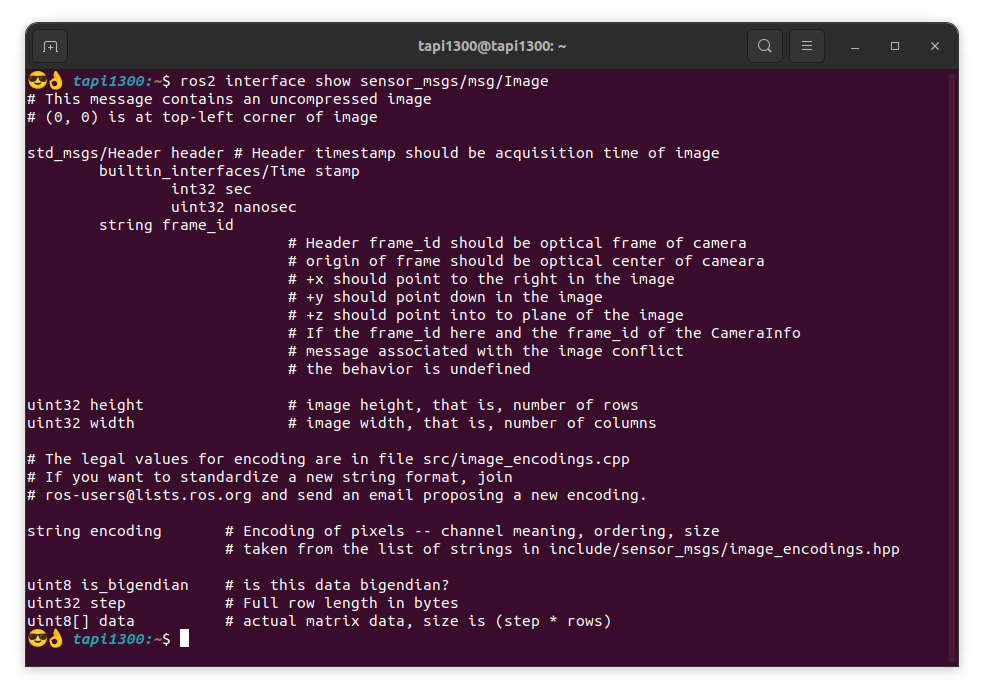
\includegraphics[width=10cm]{figs/c4/image_struct.png}
  \end{center}
  \caption[Estructura mensaje Image]{Estructura de tipo de mensaje \textit{sensor\_msgs/msg/Image}.}
  \label{fig:image_struct}
\end{figure}
Podemos ver en la figura \ref{fig:image_struct} que la imagen que obtendremos estará en el campo \textit{data} del mensaje, pero ROS tiene una
función llamada \textit{CvBridge}\footnote{\textbf{CvBridge}: \url{http://wiki.ros.org/cv_bridge}}, que nos permite transformar un mensaje del
tipo \textit{sensor\_msgs/msg/Image} en una imagen de numpy\footnote{\textbf{Numpy}: \url{https://numpy.org/}}. Como los hilos de VisualCircuit
comparten las imágenes como un array de numpy, debemos convertir la imagen de numpy a un array de numpy, usando la función \textit{numpy.asarray}.
\begin{code}[H]
  \begin{lstlisting}[language=python]
    class CamSubscriber(Node):
        def __init__(self, topic):
            super().__init__('cam_subscriber')
            self.subscription = self.create_subscription(
                Image, topic, self.callback, 10)
            self.subscription  # prevent unused variable warning
        def callback(self, msg):
            global frame
            frame = np.asarray(bridge.imgmsg_to_cv2(msg, "bgr8"), dtype=np.uint8)
  \end{lstlisting}
  \caption[Clase del nodo suscriptor para cámara]{Clase del nodo suscriptor para la cámara.}
  \label{cod:cam_node_class}
\end{code}
En cuanto a la función main, sólo habría que cambiar la función que usamos para compartir, ya que ahora compartimos una imagen:
\begin{code}[H]
  \begin{lstlisting}[language=python]
  while auto_enable or inputs.read_number('Enable'):
      frame =  None
      rclpy.spin_once(camera_subscriber)
      if frame is not None:
          outputs.share_image("Out", frame)
  \end{lstlisting}
  \caption[Cambios main bloque cámara]{Cambios a la función main del bloque driver de la cámara.}
  \label{cod:cam_main_changes}
\end{code}
% ****** LASER
Para el láser, podemos hacer lo mismo que con la cámara y revisar la estructura del tipo de mensaje, en este caso usando ``\lstinline|ros2 interface show sensor_msgs/msg/LaserScan|":
\begin{figure} [H]
  \begin{center}
      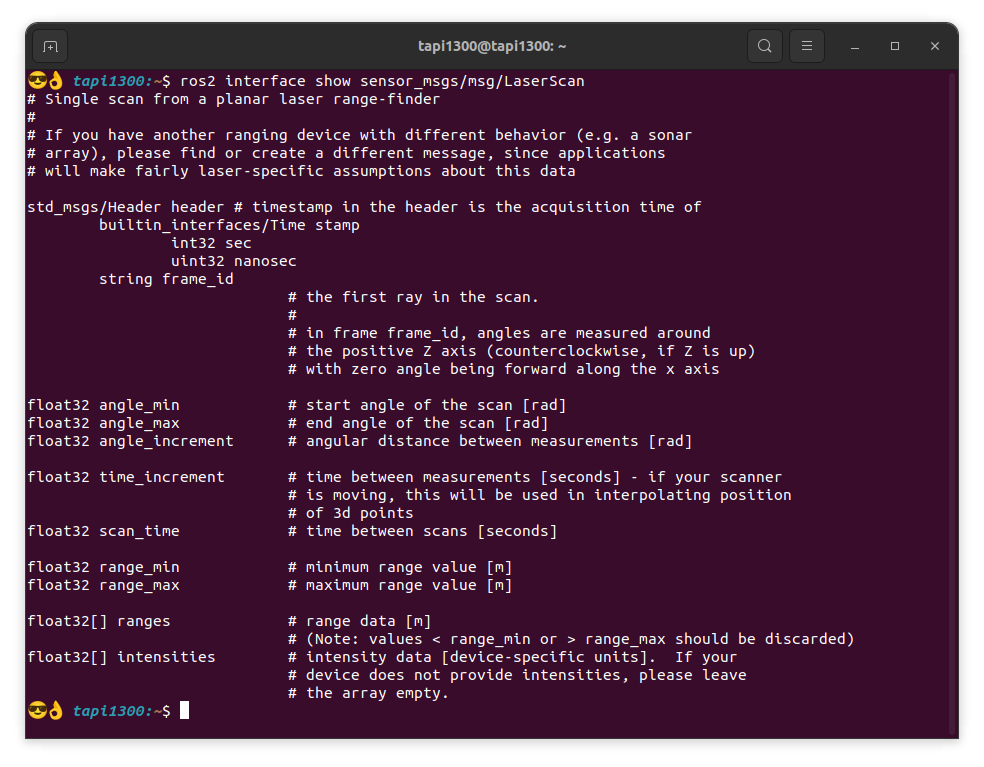
\includegraphics[width=10cm]{figs/c4/laserscan_struct.png}
  \end{center}
  \caption[Estructura mensaje LaserScan]{Estructura de tipo de mensaje \textit{sensor\_msgs/msg/LaserScan}.}
  \label{fig:laserscan_struct}
\end{figure}
Podemos ver en la figura \ref{fig:laserscan_struct} que la lectura del láser estará en el campo \textit{ranges} del mensaje, que es un \textit{array}
de \textit{floats} por lo que, para guardarlo en un array local usaremos la función de python ``\textit{.extend()}", que nos permite añadir una entrada
más a un array. Esto lo haremos en el callback, ya que es donde actualizamos el valor de la variable global.
\begin{code}[H]
  \begin{lstlisting}[language=python]
    class LaserSubscriber(Node):
        def __init__(self, topic):
            super().__init__('laser_subscriber')
            self.subscription = self.create_subscription(
                LaserScan, topic, self.callback, 10)
            self.subscription  # prevent unused variable warning
        def callback(self, msg):
            global measure
            measure = []
            for i in range(len(msg.ranges)):
                measure.extend((str(msg.ranges[i]),))
  \end{lstlisting}
  \caption[Clase del nodo suscriptor para láser]{Clase del nodo suscriptor para el láser.}
  \label{cod:laser_node_class}
\end{code}
En cuanto a la función main, sólo habría que cambiar la función que usamos para compartir, ya que ahora compartimos un array:
\begin{code}[H]
  \begin{lstlisting}[language=python]
    while auto_enable or inputs.read_number('Enable'):
        measure = None
        rclpy.spin_once(laser_subscriber)
        if measure is not None:
            outputs.share_array("Out",measure)   
        synchronise()  
  \end{lstlisting}
  \caption[Cambios main bloque láser]{Cambios a la función main del bloque driver del láser.}
  \label{cod:laser_main_changes}
\end{code}

% ******** MOTOR DRIVER
Ya tenemos los bloques de los sensores, pero aún nos queda el que corresponde a los motores.
En este caso, la configuración del bloque será distinta, ya que no necesitamos salida y sí necesitamos una entrada para que nos
digan qué velocidades mandar al robot. Por esto, tendremos un bloque de código, un parámetro para el \textit{topic} de ROS2 y dos
entradas, una para \textit{enable} (máquinas de estados) y otra para las velocidades que debemos enviar.\\

\newpage
El tipo de mensaje que suelen admitir los robots es ``geometry\_msgs/msg/Twist", y si miramos su estructura usando ``\lstinline|ros2 interface show geometry_msgs/msg/Twist|",
nos encontramos lo siguiente:
\begin{figure} [H]
  \begin{center}
      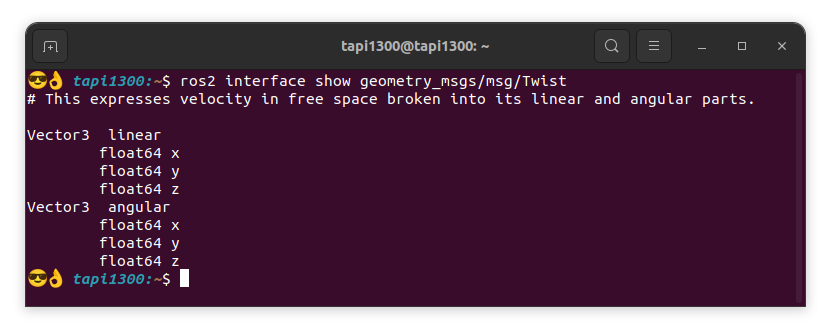
\includegraphics[width=10cm]{figs/c4/twist_struct.png}
  \end{center}
  \caption[Estructura mensaje Twist]{Estructura de tipo de mensaje \textit{geometry\_msgs/msg/Twist}.}
  \label{fig:twist_struct}
\end{figure}

Como podemos ver en la figura \ref{fig:twist_struct}, este tipo de mensajes lleva dos paquetes de 3 floats, el primero para las velocidades
lineales y el segundo para las angulares. Para crear un bloque más general que pueda adaptarse a todo tipo de robots, el bloque recibirá un array
de 6 floats permitiendo introducir velocidades lineales y angulares en las 3 dimensiones que nos permite el mensaje, ya que aunque la mayoría de
robots terrestres sólo usen una velocidad lineal y una angular, así permitimos el uso de este bloque con otros robots como drones o robots con ruedas
omnidireccionales.\\

Para poder crear el nodo publicador iremos, al igual que hicimos con el suscriptor, a los manuales de
ROS2-humble\footnote{\url{https://docs.ros.org/en/humble/Tutorials/Beginner-Client-Libraries/Writing-A-Simple-Py-Publisher-And-Subscriber.html\#write-the-publisher-node}} y
a partir de ahí crear nuestro nodo publicador.













\begin{code}[H]
  \begin{lstlisting}[language=python]
    import numpy as np
    import rclpy
    from rclpy.node import Node
    from cv_bridge import CvBridge
    from geometry_msgs.msg import Twist

    bridge = CvBridge()
    velocities = 0

  \end{lstlisting}
\end{code}
\begin{code}[H]
  \begin{lstlisting}[language=python]
    # ros2 node class
    class VelPublisher(Node):
        def __init__(self, topic):
            super().__init__('vel_publisher')
            self.publisher_ = self.create_publisher(Twist, topic, 1)
            timer_period = 0.5  # seconds
            self.timer = self.create_timer(timer_period, self.timer_callback)
        def timer_callback(self):
            global velocities
            msg = Twist()
            try:
                msg.linear.x = float(velocities[0])
                msg.linear.y = float(velocities[1])
                msg.linear.z = float(velocities[2])
                msg.angular.x = float(velocities[3])
                msg.angular.y = float(velocities[4])
                msg.angular.z = float(velocities[5])
            except IndexError:
                print("bad length for input array")
                return
            self.publisher_.publish(msg)

    def main(inputs, outputs, parameters, synchronise):
        global velocities
        auto_enable = False
        try:
            enable = inputs.read_number('Enable')
        except Exception:
            auto_enable = True
        rclpy.init()
        vel_publisher = VelPublisher(parameters.read_string('ROSTopic'))
        try:
            while auto_enable or inputs.read_number('Enable'):
                velocities = inputs.read_array('Vels')
                if velocities != None:
                    rclpy.spin_once(vel_publisher) 
                synchronise()   
        except KeyboardInterrupt:
            vel_publisher.destroy_node()
            rclpy.shutdown()
  \end{lstlisting}
  \caption[Bloque MotorDriverROS2]{Bloque MotorDriverROS2 completo.}
  \label{cod:motordriverros2_all}
\end{code}

Al ser un publicador, funciona con un temporizador para publicar el mensaje actualizado. Como podemos ver, se lee un array, se guarda en
la variable global y cuando vuelva a ejecutarse el temporizador, se enviará la última actualización de las velocidades.















\chapter{Sigue personas}
\label{cap:capitulo5}
Ahora que ya tenemos integrado ROS2 dentro de la plataforma de VisualCircuit, vamos a crear varios proyectos usando los bloques drivers que hemos creado.
El primero de ellos será un comportamiento de \textit{follow-person} usando reconocimiento visual.

\section{Desarrollo inicial sigue-personas (sólo rotación)}
\label{sec:FP_intro}

El comportamiento sigue-persona que buscamos desarrollar con VisualCircuit consiste en rotar en círculos hasta encontrar a una persona mediante
algoritmos de detección visual de objetos y mantener a la persona centrada en la imagen, al igual que mantenernos a una distancia constante,
usando así la función de lectura de distancias de la cámara. Por ello sólamente la cámara como sensor, ya que esta función mencionada nos permite no
usar el láser y evitar un código más complejo.\\

En una primera aproximación, buscaremos sólo mantener a la persona centrada usando únicamente movimiento angular y, una vez que tengamos esta parte funcionando,
añadiremos la parte del comportamiento que implica seguir a la persona también linealmente.\\

En primer lugar, debemos preparar el entorno de pruebas, por lo que aprovecharemos un modelo de persona teleoperada que creó Carlos
Caminero\footnote{\url{https://github.com/RoboticsLabURJC/2021-tfg-carlos-caminero/tree/main/amazon_hospital/hospital_world}}, compañero de la carrera.

\begin{figure} [H]
    \begin{center}
        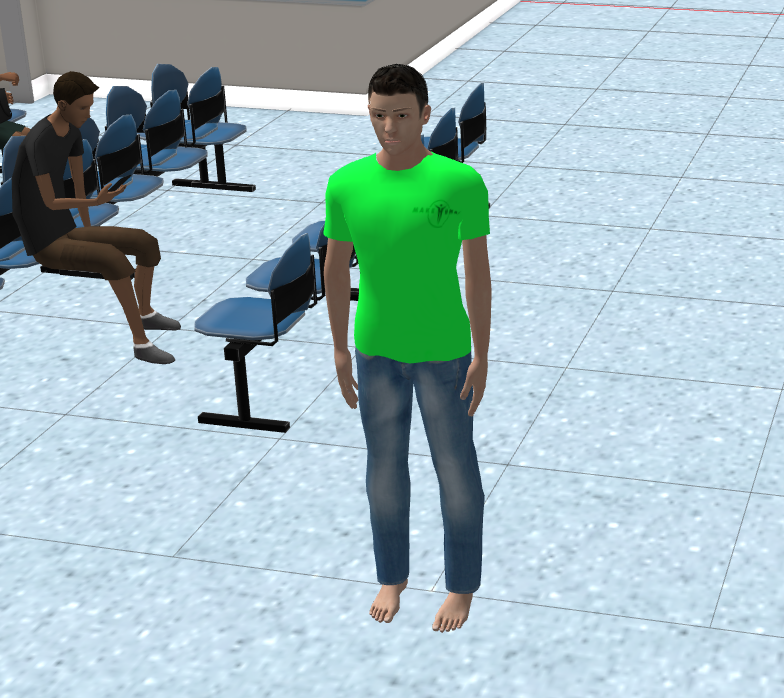
\includegraphics[width=7cm]{figs/c5/elman.png}
    \end{center}
    \caption[Modelo de persona en gazebo]{Modelo de persona teleoperable en gazebo.}
    \label{fig:teleop_person}
\end{figure}
El mundo que tenía Carlos creado incluía muchos elementos del entorno que no son necesarios en nuestro caso, por lo que modificaremos el
mundo para dejar únicamente al robot y a la persona. El modelo del robot que usaremos será el que mencionamos en el capítulo \ref{subsec:turtlebot2_sim},
ya que incluye tanto cámara como láser.\\

\begin{figure} [H]
    \begin{center}
        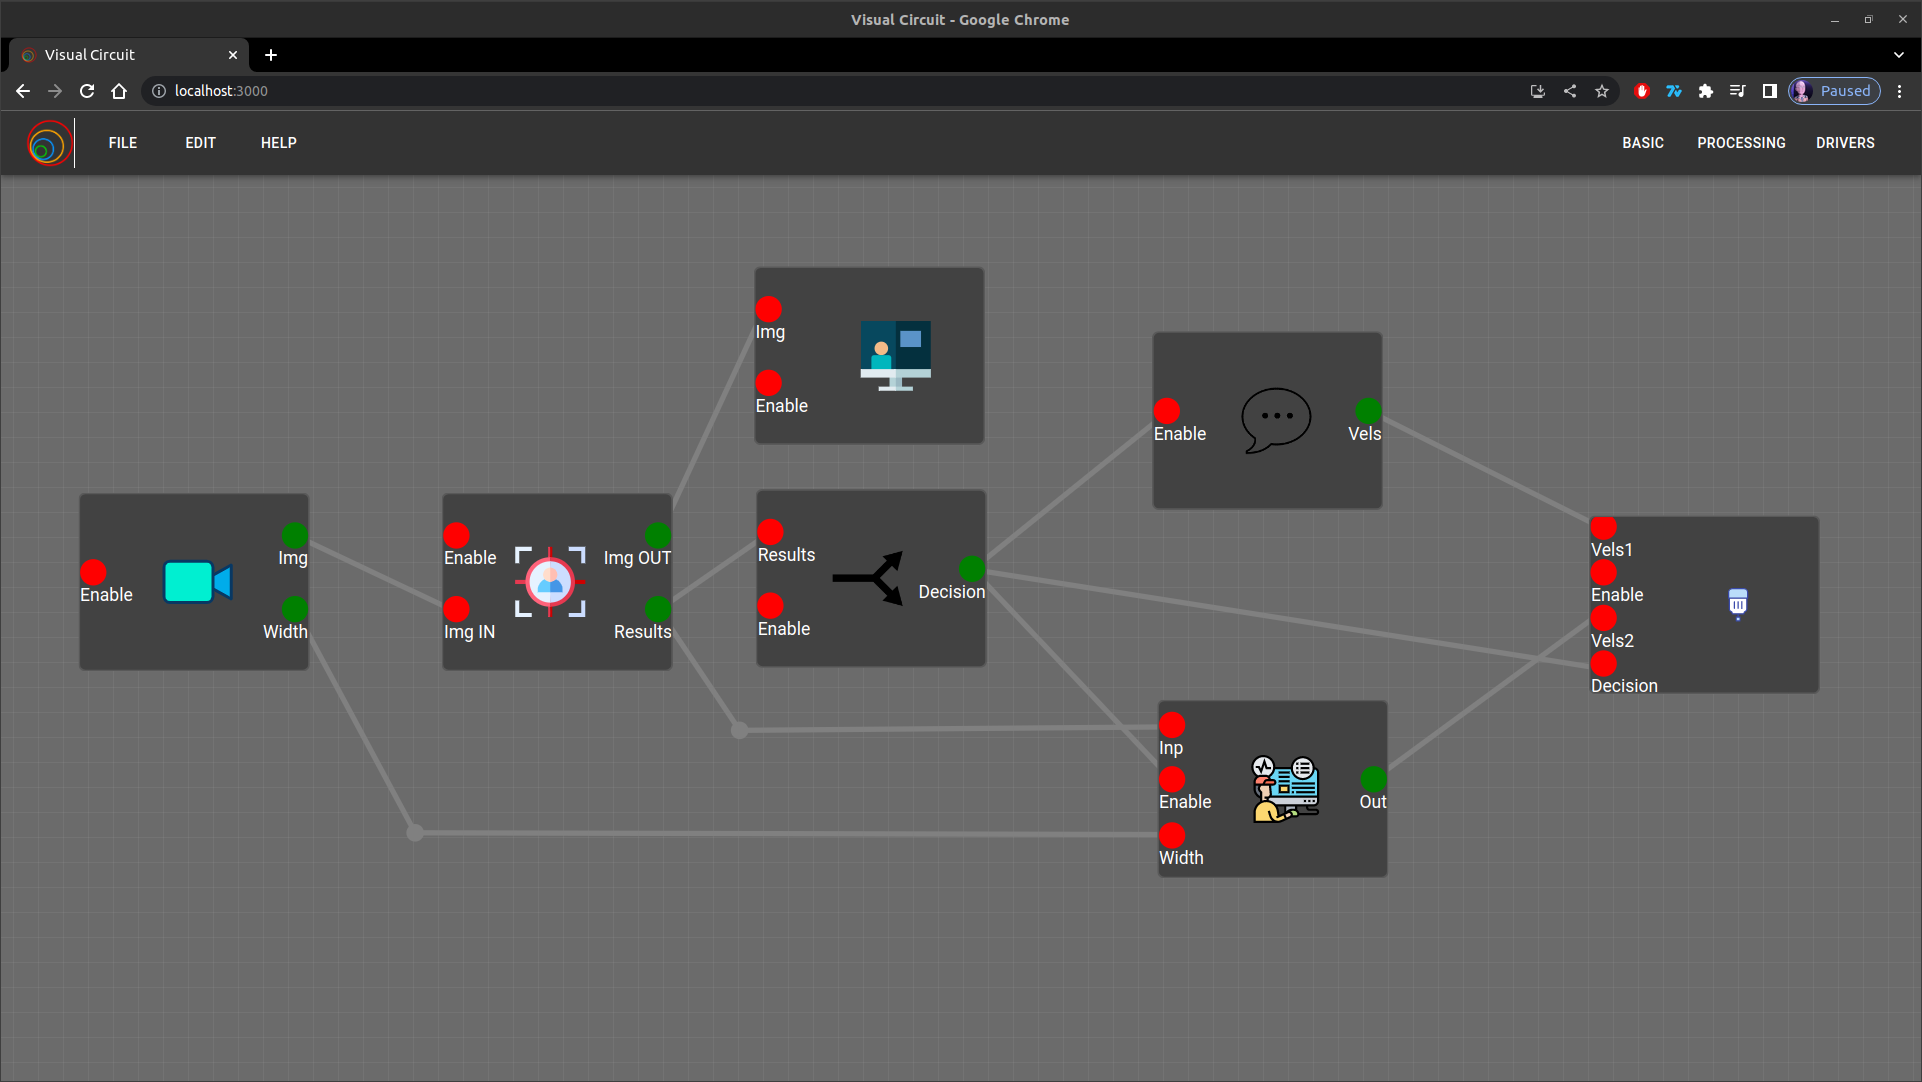
\includegraphics[width=12cm]{figs/c5/follow_person_initial.png}
    \end{center}
    \caption[Circuito sigue-personas inicial]{Circuito inicial del algoritmo sigue-persona.}
    \label{fig:initial_follow_person}
\end{figure}

La lógica que seguirá será la siguiente: recibir la imagen del \textit{topic} de la cámara y compartirla con el bloque de detección de objetos,
enviar la imagen con las detecciones al bloque \textit{screen} para visualizar en tiempo real lo que está analizando el robot,
y también mandaremos los resultados a un bloque que decidirá qué hacer. Este bloque activa un PID en caso de que haya una persona en la imagen,
o el comportamiento de rotación en caso de que no se haya encontrado ninguna.
En ambos casos, se envía la decisión a los bloques que generan las velocidades y también al bloque \textit{MotorDriver} que hemos creado en
el punto \ref{sec:drivers_creacion}, que recibe tanto las distintas velocidades, como la decisión que se ha tomado, y envía al \textit{topic} la adecuada.

La detección visual utiliza yolov3\footnote{\textbf{YouOnlyLookOnce (YOLO)}: \url{https://pjreddie.com/darknet/yolo/}},
un algoritmo de detección de objetos a tiempo real que permite identificarlos tanto en video como en imágenes usando redes neuronales
(darknet\footnote{\textbf{DarkNet}: \url{https://pjreddie.com/darknet/}}). El bloque que ya está integrado en VisualCircuit nos sirve para nuestra aplicación,
pero he tenido que modificarlo para poder extraer también la localización de la \textit{Bounding Box} que corresponde a la persona y compartirla con otros bloques.\\

Para ello, después de obtener los nombres de los objetos encontrados, recorremos toda la lista comprobando si hay alguna persona,
en caso de haberla enviamos la \textit{Bounding Box} correspondiente, sino, enviamos un \textit{array} con cuatro valores ``-1'' para indicar que está vacío.

\begin{code}[H]
    \begin{lstlisting}[language=python]
    #**********
        #forward Pass
        results = net.forward(outputNames)
        findObjects(results,frame)
        is_person = False
        for i in classIds:
            if(className[i] == "person"):
                is_person = True
                break
        to_send = [-1,-1,-1,-1]
        if(is_person):
            to__send = bbox[i]
        outputs.share_image("Img OUT", frame)
        outputs.share_array("Results", to__send)
        synchronise()
    #**********
    \end{lstlisting}
    \caption[Modificación al bloque detector de objetos]{Modificación al bloque de la detección de objetos.}
    \label{cod:mod_object_detector}
\end{code}

El siguiente bloque (\ref{cod:decision_follow_person}) es el que toma las decisiones de qué comportamiento seguir.
Para ello, primero esperaremos hasta recibir algún resultado de la visión y así no movernos antes haber podido analizar la situación.\\
Una vez que tengamos resultados, miraremos si es una \textit{Bounding Box} válida, en caso de serlo, la decisión será seguir lo que indique el bloque PID.
En caso de ser una caja vacía (\textit{array} de ``-1'') activaremos un contador para aplicar un filtro de paso bajo.\\
Este filtro nos permite evitar cambiar de comportamiento por pequeños errores en la detección de objetos.
Está establecido a 10, por lo que al llegar a 10 imágenes seguidas sin una persona en la imágen, cambiaremos de comportamiento al de la rotación.\\

\begin{code}[H]
    \begin{lstlisting}[language=python]
        def main(inputs, outputs, parameters, synchronise):
            auto_enable = True
            try:
                enable = inputs.read_number("Enable")
            except Exception:
                auto_enable = True
             
            while(True):
            # Wait for results
                results = inputs.read_array("Results")
                try:
                    if(results.any()):
                        break
                except Exception:
                    continue
    
            not_to_enable = 0
            to_enable = 1
            lowpass_filter = 10
            counter = 0
            print("EMPEZAMOS")

            while(auto_enable or inputs.read_number('Enable')):
                results = inputs.read_array("Results")
                if(results[0] != -1):
                    # Follow
                    counter = 0
                    outputs.share_number("Decision", 1)
                elif(counter < lowpass_filter):
                    # Follow but low-pass filter
                    counter += 1
                    outputs.share_number("Decision", 2)
                else:
                    # Rotation
                    outputs.share_number("Decision", 0)
    \end{lstlisting}
    \caption[Código bloque decisión sigue-persona]{Código del bloque de decisiones del sigue-persona.}
    \label{cod:decision_follow_person}
\end{code}

En cuanto al bloque que envía la velocidad correspondiente al comportamiento de rotación, tiene un bucle que lee el cable que le llega, en caso de
ser un "1" (\textit{True}) informa en la terminal que estamos rotando y envía una velocidad angular de 1rad/s para el eje Z.

\begin{code}[H]
    \begin{lstlisting}[language=python]
    import numpy as np

    def main(inputs, outputs, parameters, synchronise):
        try:
            while 1:
                if(inputs.read_number('Enable')):
                    print("ROT")
                    vels = [0,0,0,0,0,1]
                    to_write = np.array(vels, dtype='<U64')
                    outputs.share_array("Vels", to_write)   
                    synchronise()
        except Exception as e:
            print("Error")
    \end{lstlisting}
    \caption[Código bloque rotación sigue-persona]{Código del bloque de la rotación del sigue-persona.}
    \label{cod:rotation_follow_person}
\end{code}

En paralelo al anterior, también se puede activar el bloque PID\footnote{
    \textbf{PID}: Controlador proporciona, integral y derivativo.
        Mecanismo de control que, mediante sistema en lazo cerrado (realimentación), permite regular
        un valor (velocidad, temperatura, presión, etc)}.
Su estructura consiste en tres entradas (Resultados de la detección de objetos, ancho de la imagen y \textit{enable}), tres parámetros para las
tres constantes del controlador y una salida para la velocidad lineal y angular final que aplicaremos al robot.

\begin{figure} [H]
    \begin{center}
        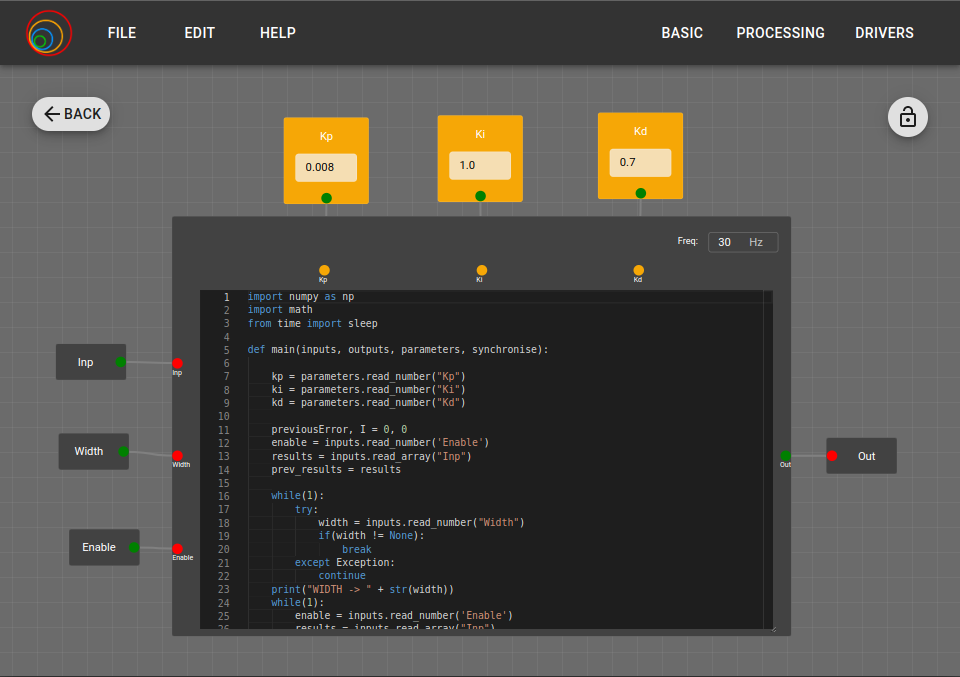
\includegraphics[width=10cm]{figs/c5/PID_follow_person.png}
    \end{center}
    \caption[Circuito del bloque PID sigue-persona]{Circuito del bloque PID del sigue-persona en VisualCircuit.}
    \label{fig:PID_follow_person}
\end{figure}

Analizando el código del bloque PID (\ref{cod:PID_follow_person}), podemos ver que primero lee los tres parámetros del controlador y entramos en el
mismo bucle que hemos mencionado en el código bloque de decisión (\ref{cod:decision_follow_person}), donde esperamos hasta obtener datos para
empezar a trabajar. Después, en el bucle principal sólo se analizan y envían los datos del PID en caso de que el bloque haya sido activado.\\

\begin{code}[H]
    \begin{lstlisting}[language=python]
        def main(inputs, outputs, parameters, synchronise):
            kp = parameters.read_number("Kp")
            ki = parameters.read_number("Ki")
            kd = parameters.read_number("Kd")
            previousError = 0
            I = 0
            max_rotation = 1
            enable = inputs.read_number('Enable')
            results = inputs.read_array("Inp")
            prev_results = results
        
            #Wait for values
            while(1):
                try:
                    width = inputs.read_number("Width")
                    if(width != None):
                        break
                except Exception:
                    continue
            while(1):
                enable = inputs.read_number('Enable')
                results = inputs.read_array("Inp")
                if(enable != 0):
                    try:        
                        if(enable == 1):
                            error = float(results[0]+results[2]/2) - width/2
                            prev_results = results
                        P = error
                        D = float(error) - float(previousError)
                        PIDvalue = (kp*P)  + (kd*D)
                        previousError = float(error)

                        angular_velocity = -PIDvalue
                        if(angular_velocity > max_rotation or angular_velocity < -max_rotation):
                            angular_velocity = max_rotation*angular_velocity/abs(angular_velocity)
                        data = [0,0,0,0,0, angular_velocity]
                        outputs.share_array("Out", data)
        
                        synchronise()
                    except Exception:
                        synchronise()
                        continue
    \end{lstlisting}
    \caption[Código bloque PID sigue-persona]{Código del bloque del PID sigue-persona.}
    \label{cod:PID_follow_person}
\end{code}

\newpage
Como podemos ver en el código anterior, el controlador usado finalmente es únicamente PD (sin parte integral).
La parte proporcional se consigue mediante la resta del resultado actual y el resultado objetivo, en nuestro caso se trata del centro de la imagen,
por lo que usamos la mitad del ancho de la imagen.
Para la parte derivativa, se busca reducir los cambios bruscos, por lo que se resta el error actual con el error de la iteración anterior.\\

Una vez que tenemos la velocidad calculada, se la mandamos al bloque de los motores. Este bloque es igual que el que creamos en el apartado
\ref{sec:drivers_creacion} pero modificado para poder tener cuatro \textit{inputs}: \textit{Enable}, vel1 (rotación), vel2 (PID) y decisión.
En el código del bloque también se ha modificado la función \textit{main} para que lea las velocidades correspondientes al comportamiento actual y
que esta sea la velocidad que se comanda a los motores del robot.\\

\begin{code}[H]
    \begin{lstlisting}[language=python]
    while auto_enable:
        try:
            decision = inputs.read_number("Decision")
            if(decision == 0):
                velocities = inputs.read_array('Vels1')
            else:
                velocities = inputs.read_array('Vels2')
        except Exception:
            continue
\end{lstlisting}
\caption[Código bloque MotorDriver sigue-persona]{Código del bloque del \textit{MotorDriver} sigue-persona.}
\label{cod:MotorDriver_FP}
\end{code}

Al probarlo todo junto usando el TurtleBot2 real, podemos observar que mientras la persona está quieta, la cámara la mantiene centrada y,
cuando empieza a moverse hacia un lado, el robot gira para volver a ponerlo en el centro de la imagen.\\

En la siguiente secuencia de imágenes se puede observar el movimiento que ha seguido el robot tras la ejecución:

\begin{figure} [H]
    \begin{center}
        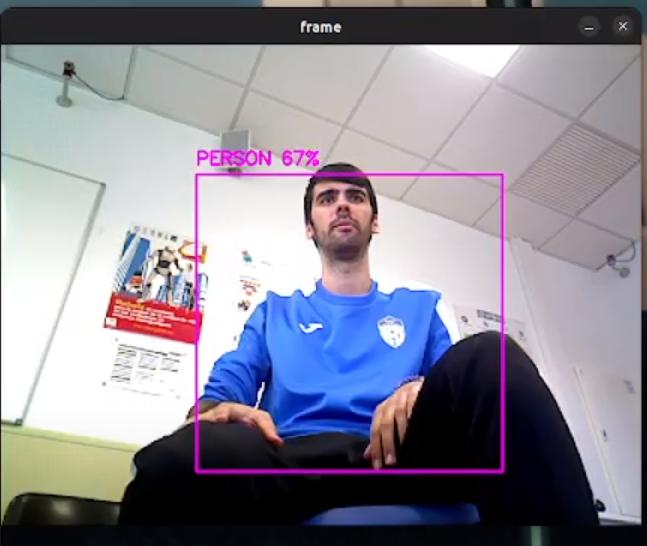
\includegraphics[width=7cm]{figs/c5/sec_rot1.png}
        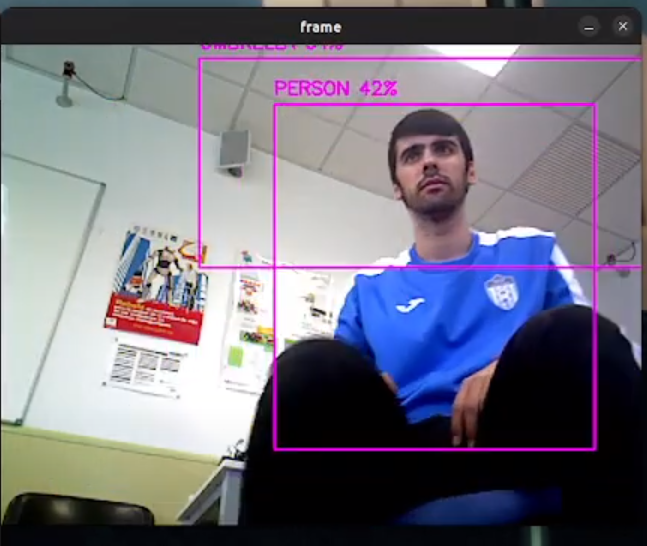
\includegraphics[width=7cm]{figs/c5/sec_rot2.png}
        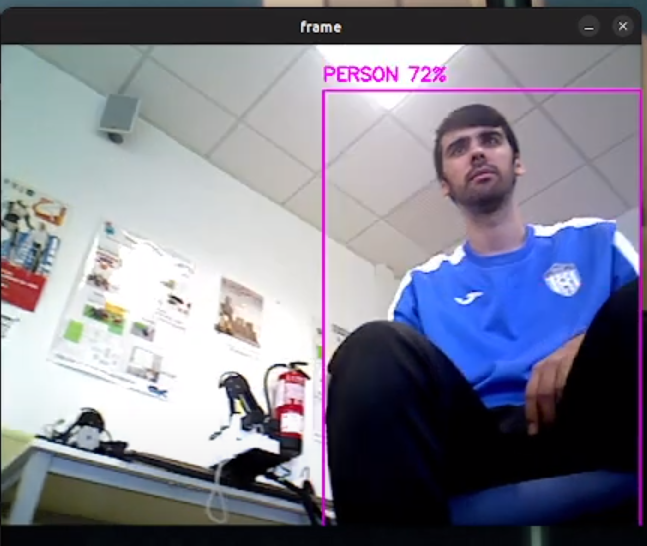
\includegraphics[width=7cm]{figs/c5/sec_rot3.png}
        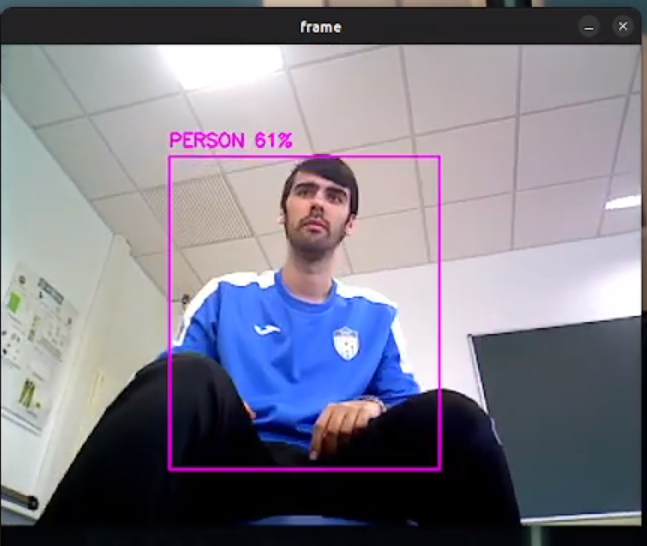
\includegraphics[width=7cm]{figs/c5/sec_rot4.png}
    \end{center}
    \caption[Secuencia sigue-personas rotación]{Secuencia de imágenes del sigue-personas. Imagenes obtenidas de Youtube\footnotemark.}
    \label{fig:sec_FP_rot}
\end{figure}
\footnotetext{\textbf{Vídeo}: \url{https://www.youtube.com/watch?v=Uir_iqMOplc&ab_channel=Tapii}}



\section{Modificaciones al sigue-personas para incluir movimiento lineal.}
\label{sec:FP_2}

Para añadir el comportamiento de seguir linealmente a la persona, debemos leer también la información sobre la profundidad que nos da la cámara.
Para ello vamos a crear un bloque usando el modelo de bloques de sensores que usamos anteriormente (\ref{sec:drivers_creacion}).
También cambiaremos el funcionamiento general de varios bloques para optimizar y reducir el número de \textit{inputs} y bloques del circuito.

\begin{figure} [H]
    \begin{center}
        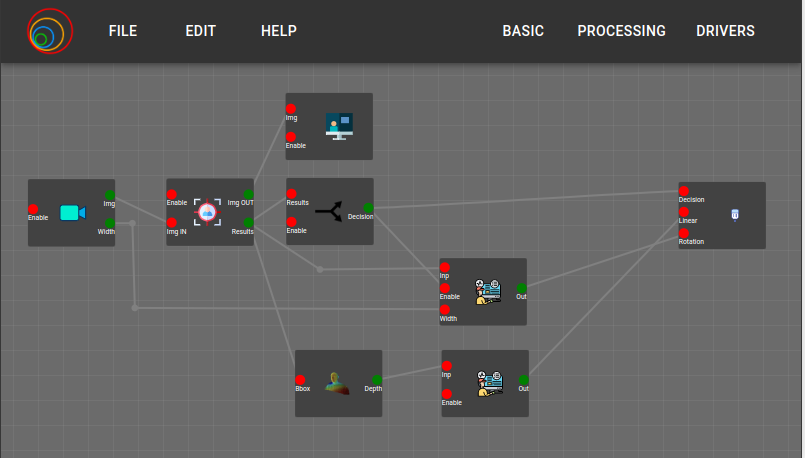
\includegraphics[width=12cm]{figs/c5/follow_person_final_model.png}
    \end{center}
    \caption[Circuito sigue-personas inicial]{Circuito inicial del algoritmo sigue-persona.}
    \label{fig:final_follow_person}
\end{figure}

Como podemos ver, toda la rama inferior de bloques es la que se encarga del movimiento lineal, mientras que la superior se encarga del movimiento angular.
La única parte de la parte superior que ha cambiado es que ya no existe un bloque que envíe siempre la velocidad de rotación, en cambio está directamente en el
bloque que envía la velocidad a los motores y, dependiendo de la decisión, se envía la rotación estática o se envían las velocidades de los bloques PID.

\begin{code}[H]
    \begin{lstlisting}[language=python]
        while auto_enable:
            try:
                decision = inputs.read_number("Decision")
                if(decision == 0):
                    velocities = [0,0,0,0,0,0.05]
                else:
                    velocities = inputs.read_array('Vels2')
                    velocities[0] = inputs.read_number('Linear')
            except Exception:
                continue

    \end{lstlisting}
    \caption[Código bloque MotorDriver sigue-persona modificado]{Código del bloque del \textit{MotorDriver} sigue-persona modificado.}
    \label{cod:MotorDriver_FP_final}
\end{code}

\begin{figure} [H]
    \begin{center}
        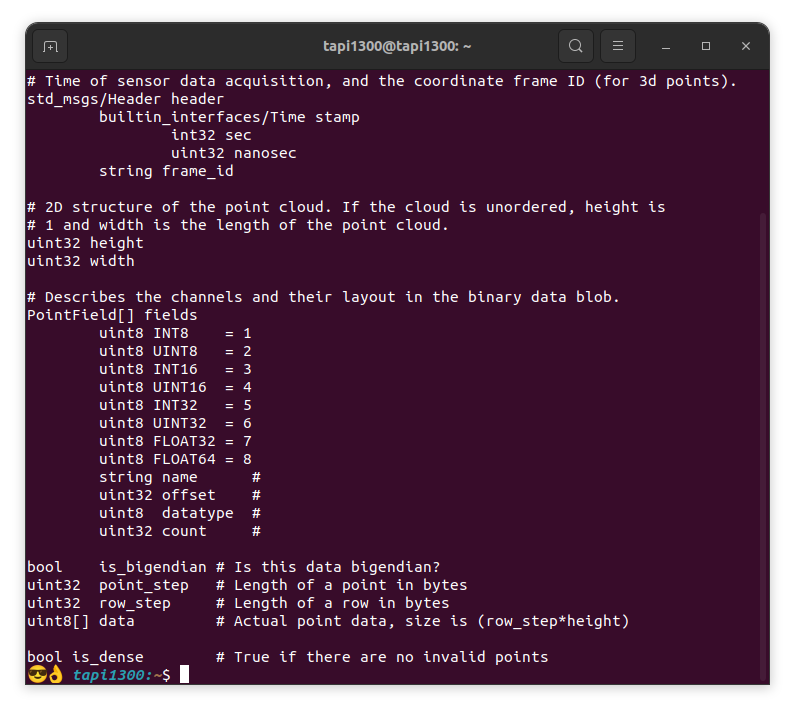
\includegraphics[width=10cm]{figs/c5/PointCloud2_data.png}
    \end{center}
    \caption[Estructura mensaje PointCloud2]{Estructura del tipo de mensaje \textit{sensor\_msgs/msg/PointCloud2.}}
    \label{fig:PC2_struct}
\end{figure}


En cuanto a la rama inferior, el bloque principal es el que recibe la información de la profundidad. Esta información viene en forma
de \textit{PointCloud2} (\textit{sensor\_msgs/msg/PointCloud2}) que, como  podemos ver en la imagen \ref{fig:PC2_struct}, envía los datos del sensor en el
campo \textit{data}, por lo que esto será lo que guardemos en la variable global del bloque del sensor y será lo que enviemos por el cable.\\

La forma en la que se guardan los datos dentro de este campo es en bytes y es la siguiente para cada punto de la cámara (640x480 = 307200 puntos):
12 bytes para x,y,z (4 bytes cada coordenada), 4 bytes vacíos, 4 bytes para el color del punto y otros 12 bytes vacíos. Esto hace que en el \textit{array} de datos
nos aparezcan 9830400 valores y la búsqueda final sea el número de filas (coordenada Y) por el ancho total de la imagen más la posición actual de nuestra coordenada X
multiplicado por 32 (posiciones que ocupa cada pixel en el array) y sumamos 8 para obtener la posición inicial de la coordenada Z. Luego, usando la función
``\textit{unpack}" del paquete \textit{struct} podemos transformar los siguiente 4 bytes (correspondientes a la coordenada Z) en un \textit{float} y obtener
la distancia entre el robot y el centro de la \textit{BoundingBox} de la persona.

\begin{code}[H]
    \begin{lstlisting}[language=python]
    # IMPORT
    from sensor_msgs.msg import PointCloud2
    from struct import unpack

    # CALLBACK DENTRO DE LA CLASE
        def callback(self, msg):
            global measure
            measure = msg.data

    # BUCLE DENTRO DEL MAIN
        while(1):
            bbox = inputs.read_array("Bbox")
            if bbox is None:
                continue
            try:
                x = int(bbox[0]+bbox[2]/2)
                y = int(bbox[1]+bbox[3]/2)
            except:
                continue

            rclpy.spin_once(depth_subscriber)
            point = (width*y+x)*32+8
            depth = unpack('f', measure[point:point+4])
            outputs.share_array("Depth",depth)   
            synchronise()
    \end{lstlisting}
    \caption[Código bloque Camera-Depth sigue-persona]{Código del bloque del \textit{PointCloud2} del sigue-persona.}
    \label{cod:PC2_block_FP}
\end{code}

Esta información llega a un segundo bloque PID, que es el que se va a encargar de mantener esta distancia con la persona en 1.5 metros. El código de este bloque
es similar al del otro bloque PID (\ref{cod:PID_follow_person}), pero ahora no necesitamos una velocidad límite (el mínimo y máximo que conseguiremos no es peligroso
en comparación a las velocidades angulares altas).

\begin{code}[H]
    \begin{lstlisting}[language=python]
        import numpy as np
        import math
        from time import sleep
        
        def main(inputs, outputs, parameters, synchronise):
            auto_enable = True
            try:
                enable = inputs.read_number("Enable")
            except Exception:
                auto_enable = True
            kp = parameters.read_number("Kp")
            ki = parameters.read_number("Ki")
            kd = parameters.read_number("Kd")
            previousError, I = 0, 0
            while(auto_enable or inputs.read_number('Enable')):
                msg = inputs.read_number("Inp")
                if msg is None:
                    continue
                error = float(msg) - 1.5
                sleep(0.01)
        
                P = error
                D = error - previousError
                PIDvalue = (kp*P) + (kd*D)
                previousError = error
    
                linear_velocity = PIDvalue
                if msg == 0:
                    linear_velocity = 0
                outputs.share_number("Out", linear_velocity)
                synchronise()
    \end{lstlisting}
    \caption[Código bloque PID lineal sigue-persona]{Código del bloque del PID de velocidad lineal del sigue-persona.}
    \label{cod:PID_linear_FP}
\end{code}



\section{Pruebas en el robot real y resultado final.}
\label{sec:FP_final}

Ahora que ya está configurado el comportamiento correctamente, tanto la velocidad lineal para mantenerse a 1.5 metros como la velocidad angular para
mantener al humano en el centro de la visión del robot, es hora de probarlo en el robot real.\\

Para configurar correctamente los sensores del robot real debemos tener instalados los paquetes referentes a lanzar el kobuki (\ref{subsec:turtlebot2_base}),
al igual que los necesarios para usar la cámara (\ref{subsec:asus_xtion}).
De aquí usaremos los siguientes comandos para conseguir que todo funcione correctamente:

\begin{code}[H]
    \begin{lstlisting}[language=bash]

$> ros2 launch asus_xtion asus_xtion.launch.py

$> ros2 launch ir_kobuki kobuki_rplidar.launch.py
    \end{lstlisting}
    \caption[Comandos para lanzar kobuki y cámara]{Comandos para activar la cámara con ROS2 y lanzar el kobuki con el laser.}
    \label{cod:coms_kobuki_laser_cam}
\end{code}

Una vez probado, podemos comprobar los resultados mirando el vídeo en el que se explica el funcionamiento de los bloques (como ya se ha explicado en las
secciones \ref{sec:FP_intro} y \ref{sec:FP_2}) y se muestra un ejemplo de ejecución con el robot real en los laboratorios:


\begin{figure} [H]
    \begin{center}
        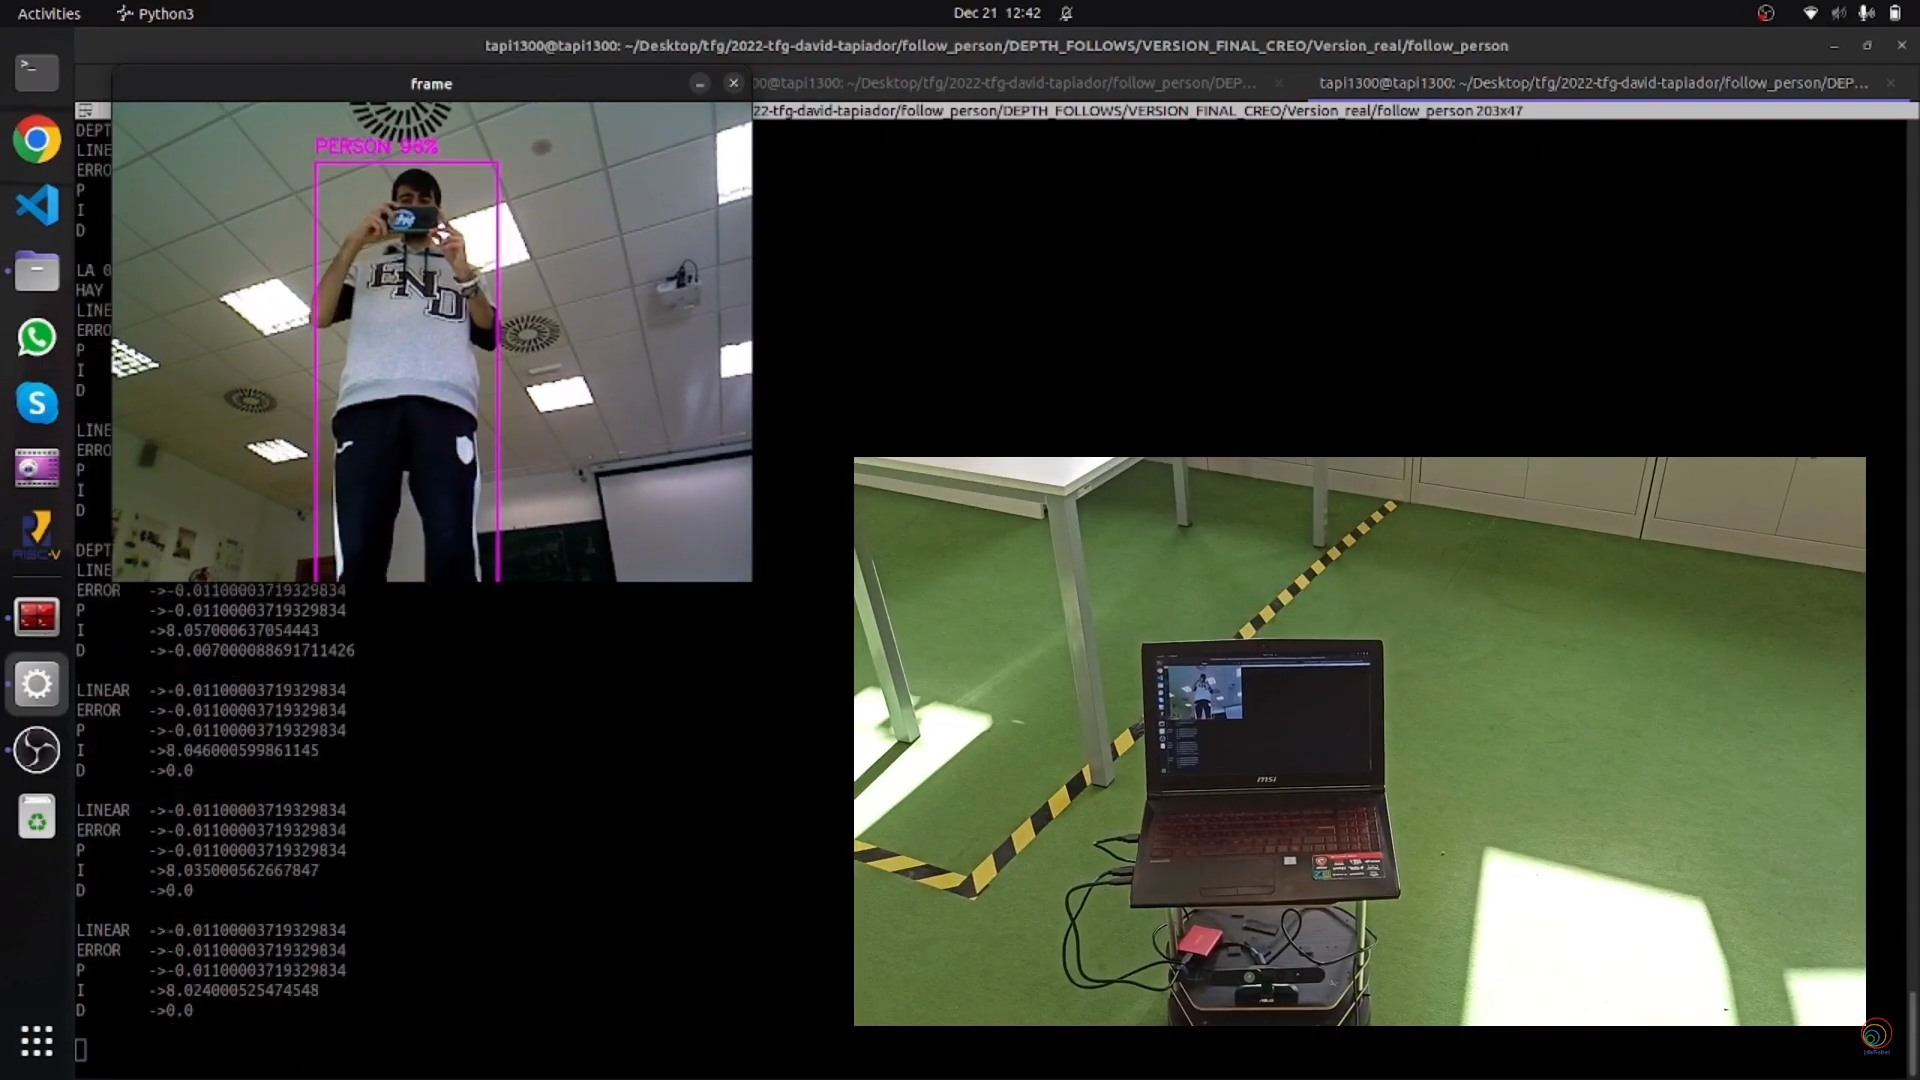
\includegraphics[width=7cm]{figs/c5/fp_final1.png}
        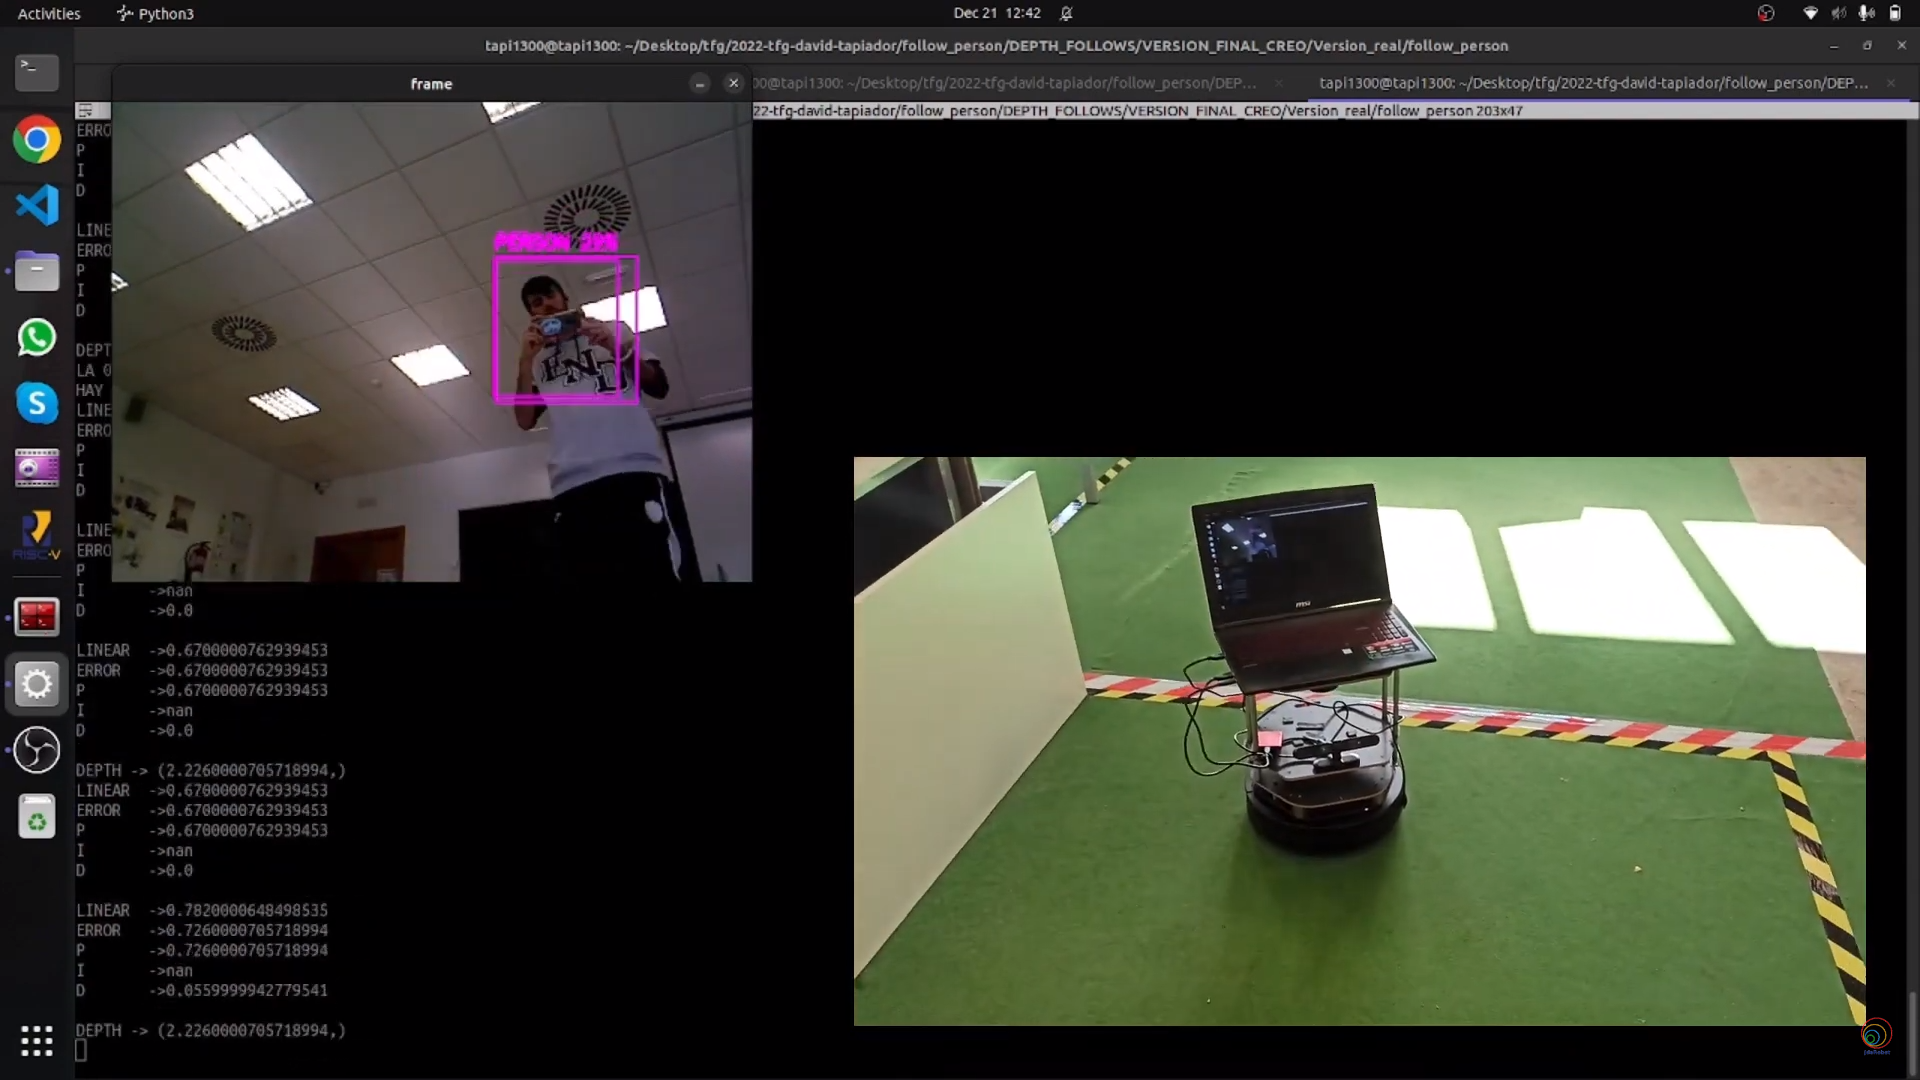
\includegraphics[width=7cm]{figs/c5/fp_final2.png}
        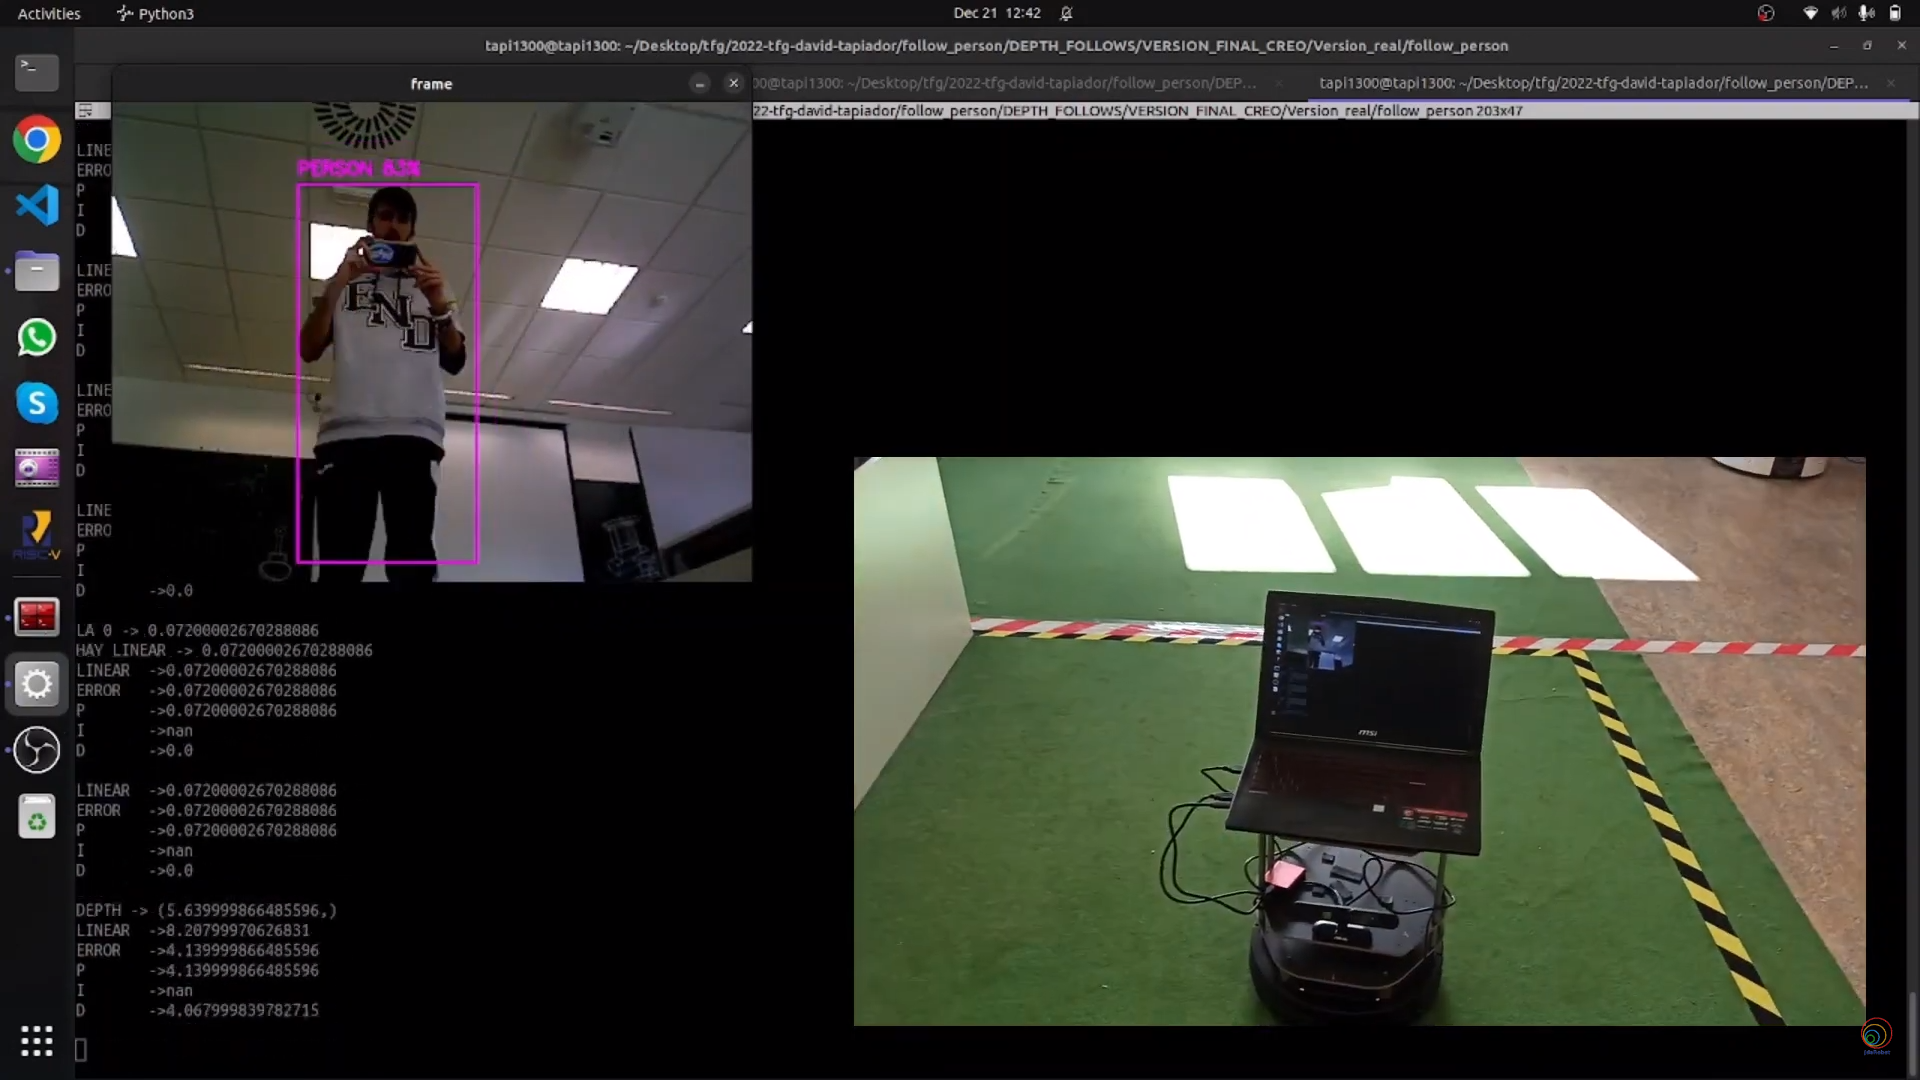
\includegraphics[width=7cm]{figs/c5/fp_final3.png}
        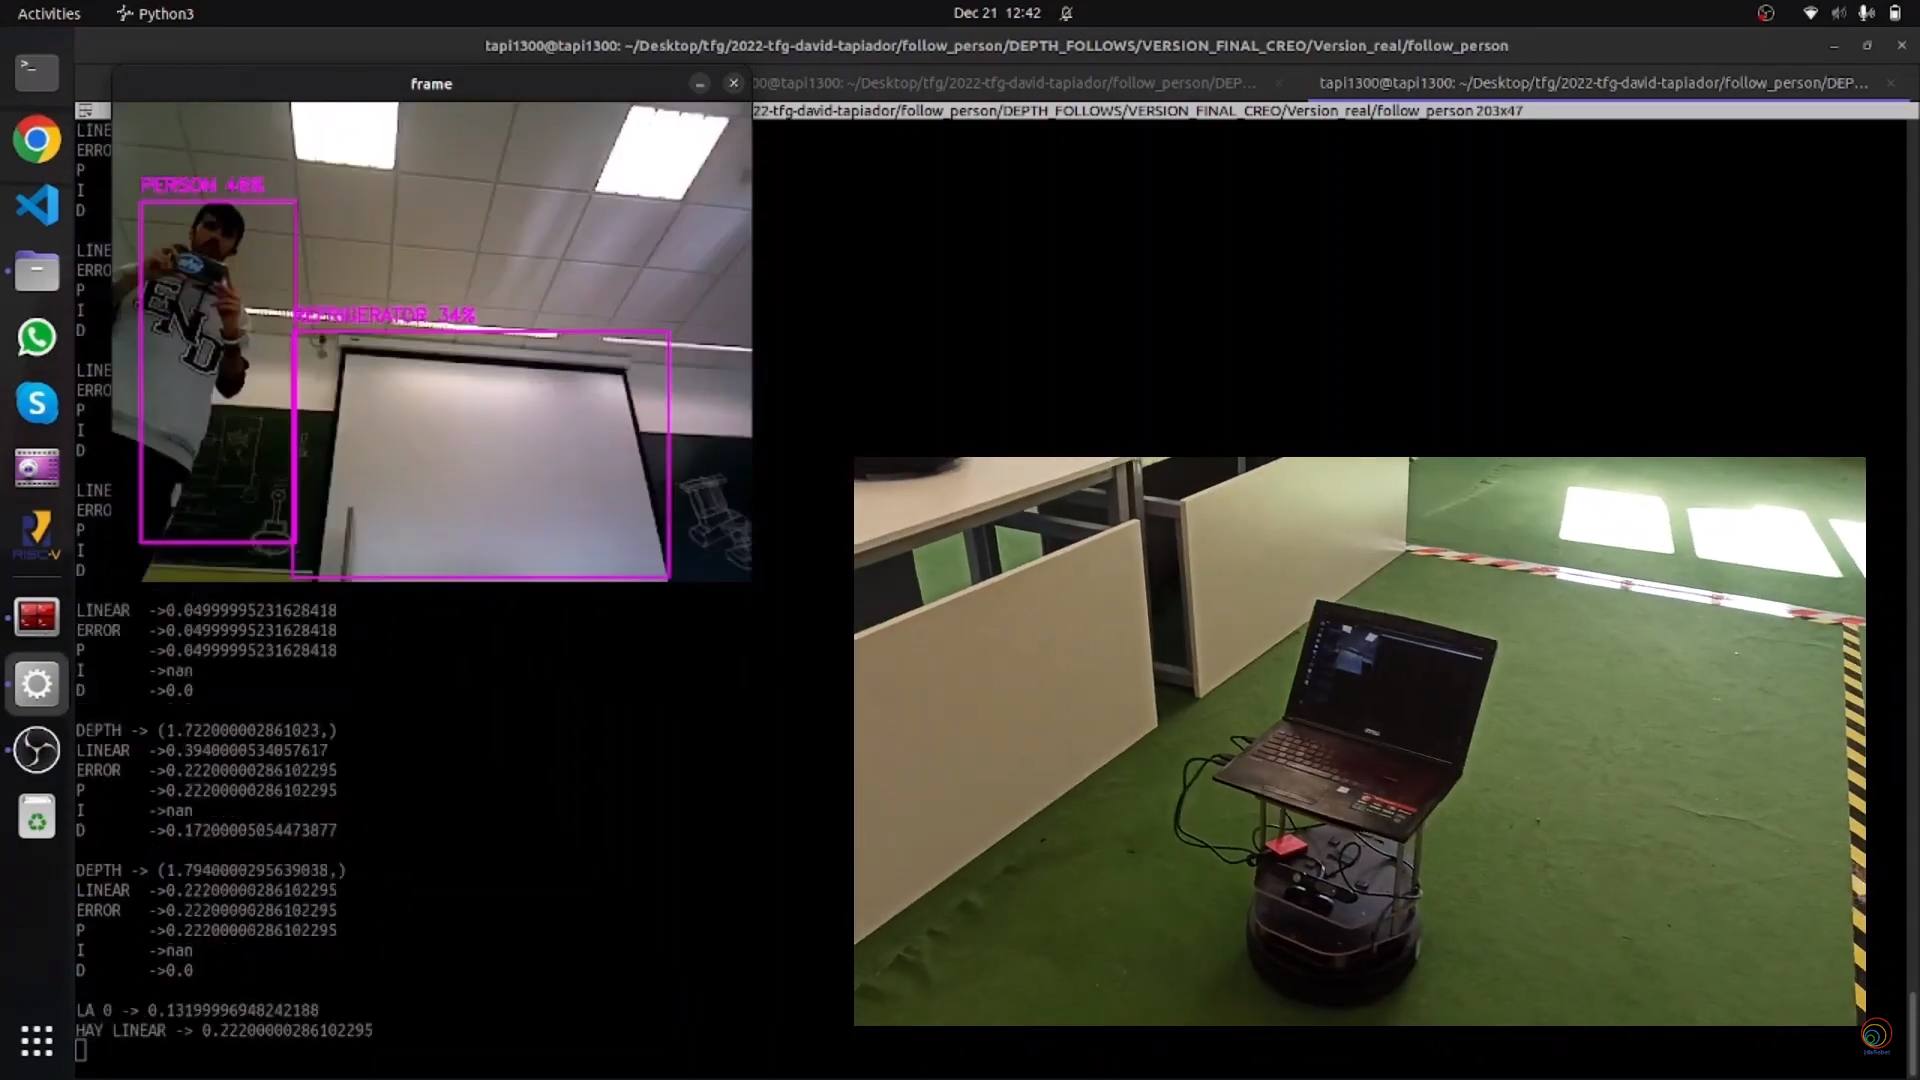
\includegraphics[width=7cm]{figs/c5/fp_final4.png}
    \end{center}
    \caption[Secuencia sigue-personas resultado final]{Secuencia de imágenes del sigue-personas. Imagenes obtenidas de Youtube\footnotemark.}
    \label{fig:sec_FP_final}
\end{figure}
\footnotetext{\textbf{Vídeo}: \url{https://www.youtube.com/watch?v=IknpvAs_jAo&ab_channel=JdeRobot}}



































































\chapter{Aplicación Virtual Force Field}
\label{cap:capitulo6}
Como ya se ha explicado, otra de las aplicaciones que se va a desarrollar consiste en navegación usando el algoritmo VFF mediante el uso de máquinas de estados.

Para desarrollar esta aplicación, el proceso se dividirá en dos partes: desarrollo del algoritmo VFF e implementación de dicho comportamiento
en una máquina de estados que genere ubicaciones aleatorias.

\section{Campo de fuerzas virtuales (VFF)}
\label{sec:VFF}

El algoritmo de movimiento mediante campo de fuerzas virtuales o \textit{virtual field force} consiste en permitir el movimiento a través de un lugar avanzando gracias a
objetivos temporales (como si fueran balizas) y esquivando los obstáculos entre la posición del robot y el objetivo mediante la fuerza repulsiva generada por las medidas
de los distintos sensores al percibir dichos obstáculos.\\

Este algoritmo se basa en dos partes principales: la fuerza repulsiva (inversamente proporcional a la distancia con los obstáculos) y la
fuerza atractiva (dirección al objetivo). Para obtener ambas fuerzas serán necesarios dos sensores: láser (fuerza repulsiva) y odometría (fuerza atractiva).\\

\subsection{Diseño del circuito y escenario}
\label{subsec:dis_bloques_VFF}

El circuito para este comportamiento consistirá de dos ramas principales, una para cada fuerza, y la unión de estas ramas mandando una velocidad final tanto lineal como angular.\\

En la rama superior esta el sensor láser junto con un bloque para obtener una única medida como resultado de todas las medidas del láser. En la inferior se encuentra el sensor
\textit{odom}, que da la posición del robot en las coordenadas del mundo simulado.
Esta medida se pasa a dos bloques: el generador de objetivos (bloque que envía el objetivo actual
y, en caso de haber llegado, envía el siguiente dentro de una lista) y el bloque que se encarga de calcular la fuerza atractiva.

Ambas ramas se juntan en un bloque que las suma teniendo en cuenta sus valores de influencia (la repulsiva debe influir más que la atractiva para evitar colisiones por
roce) y se envían como velocidades al bloque MotorDriverROS2 (\ref{sec:motordriverros2}).
\begin{figure} [H]
    \begin{center}
        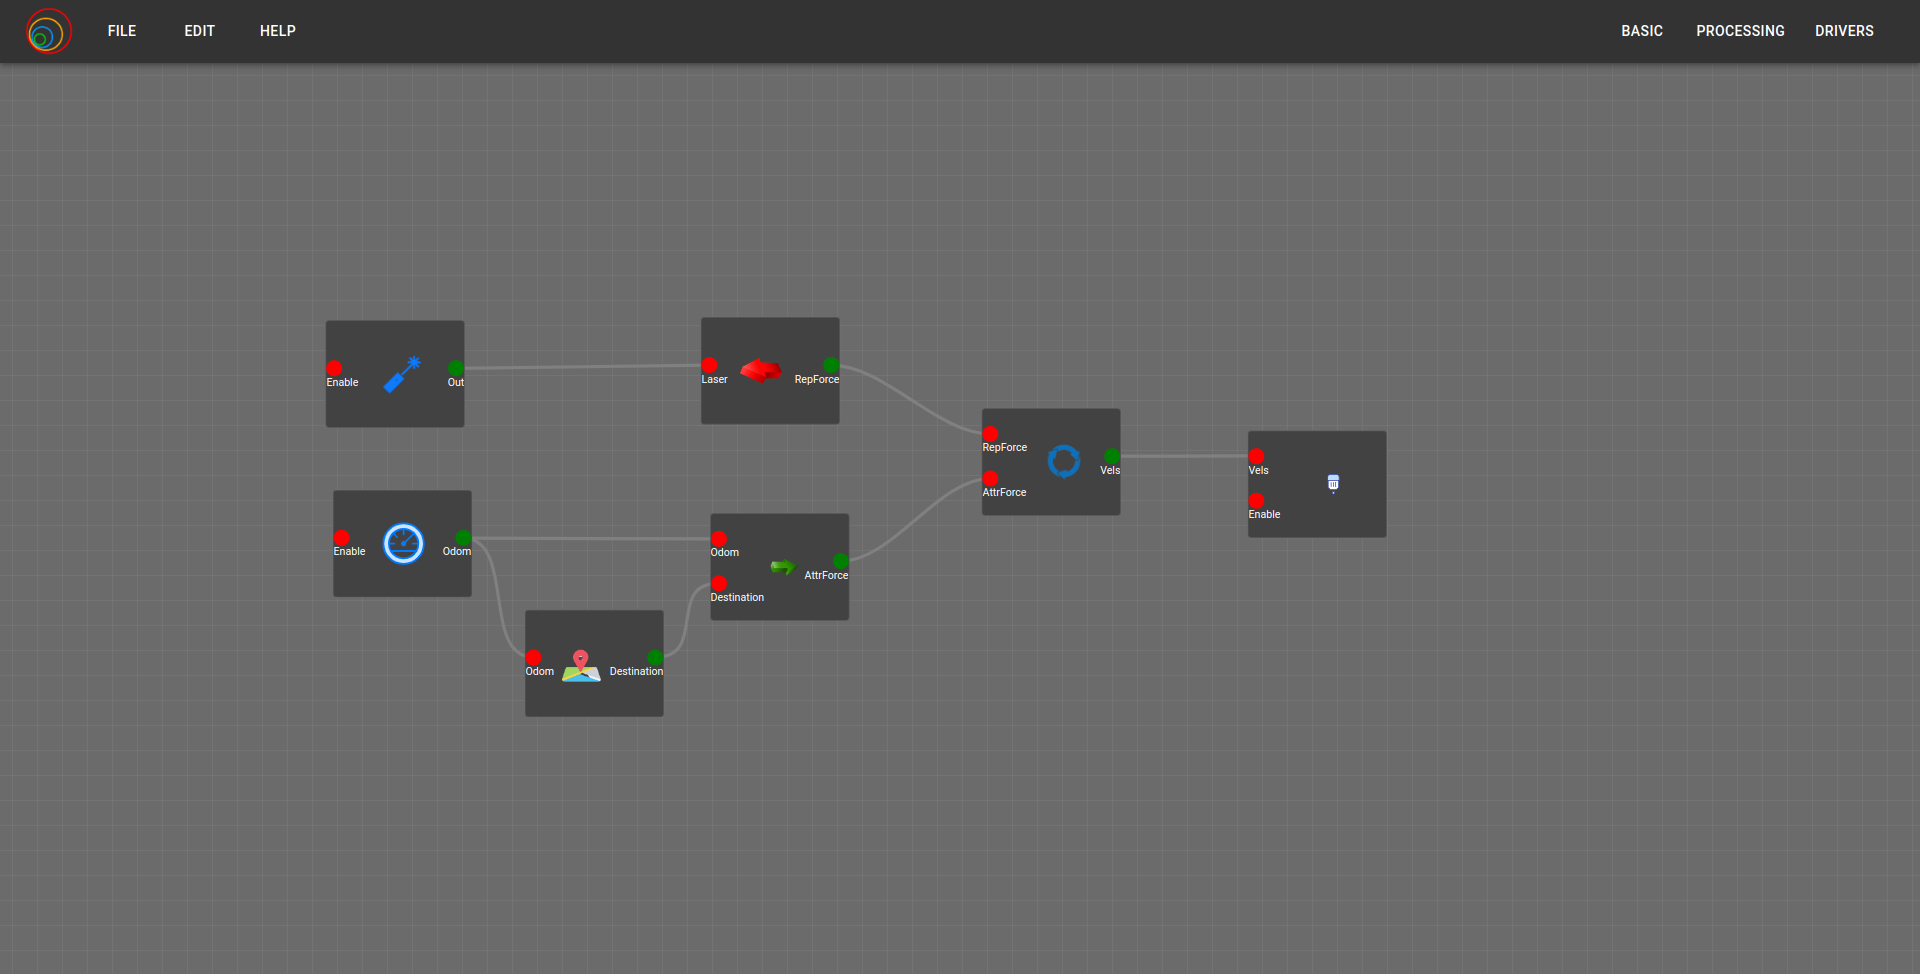
\includegraphics[width=12cm]{figs/c6/VFF_circ.png}
    \end{center}
    \caption[Circuito VFF]{Circuito del algoritmo VFF.}
    \label{fig:VFF_circ}
\end{figure}
El escenario de pruebas consistirá en un circuito creado a base de bloques cúbicos como muros con algunas barras rojas (cubos rectangulares) horizontales que marcan
aproximadamente dónde se encuentran los objetivos. Hay una zona en la que no hay practicamente borde para comprobar que la fuerza atractiva fuese lo suficiente fuerte
como para no desviarse al encontrar un hueco en uno de los lados.

\begin{figure} [H]
    \begin{center}
        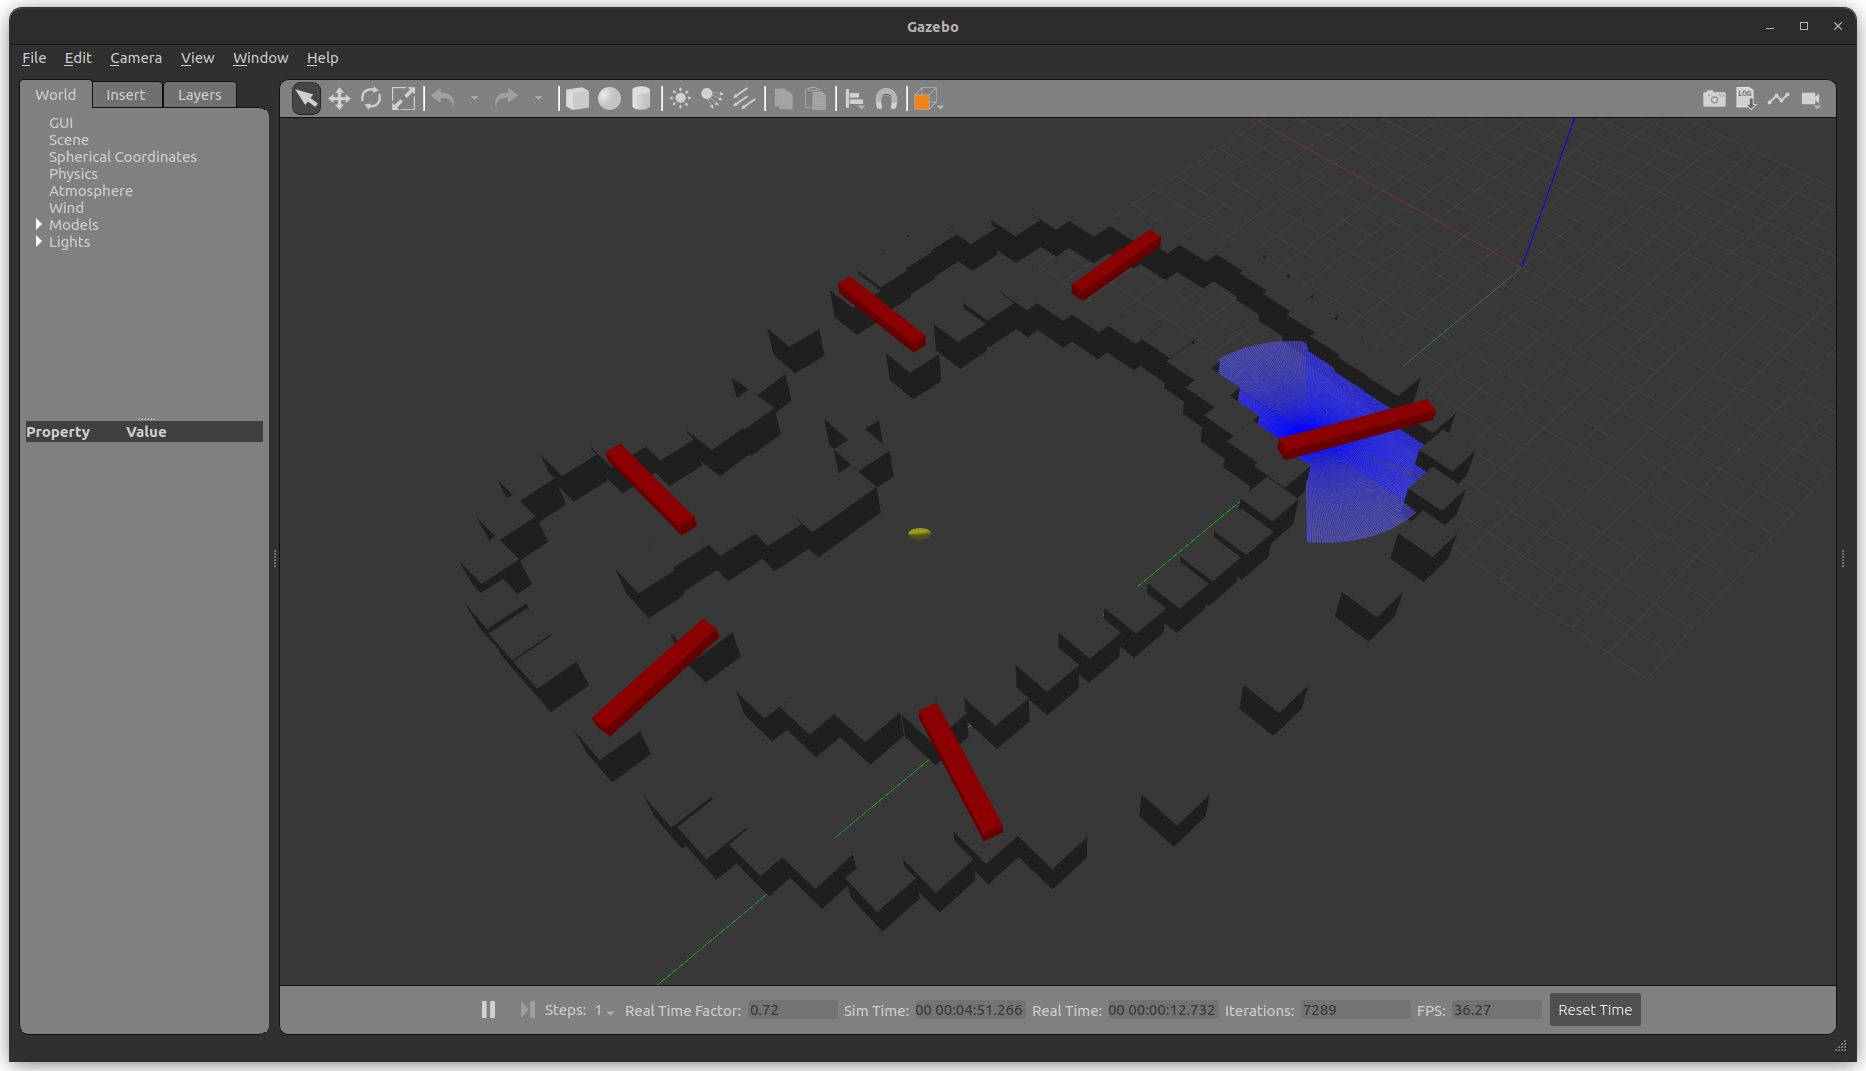
\includegraphics[width=12cm]{figs/c6/VFF_world.png}
    \end{center}
    \caption[Mundo para VFF]{Mundo gazebo para probar el algoritmo VFF.}
    \label{fig:VFF_world}
\end{figure}

\subsection{Bloques específicos}
\label{subsec:spec_bloques_VFF}

El primer bloque nuevo específico de esta aplicación es el que transforma las medidas del láser a un valor único.
Para que la información del láser sea más facilmente manipulable, se ha crea una función \textit{parse\_laser\_data()} que almacena cada medida del láser
en un array de tuplas junto al ángulo que dicha medida representa.\\

Después se recorre el array de tuplas para obtener vectores que representen el valor del eje X e Y para cada medida del láser. Ésto se hace multiplicando la medida
original (hipotenusa) por el seno o coseno del ángulo. Después se guarda en un nuevo array de tuplas para cada par de valore (x,y).\\

Ahora para calcular la fuerza final se recorre el array de medidas vectoriales sumando los valores inversos, es decir, el valor absoluto de la división de un valor
entre la medida, permitiendo que cuanto más cercano (menor sea la medida) mayor influencia tenga en el resultado de fuerza repulsiva final. En el caso del eje X, sólo
hay que comprobar que la medida sea distinta de 0, mientras que en el caso del eje Y hay que evitar medidas superiores a 10, ya que es el límite del sensor y
sumaría \textit{inf} (infinito).

\begin{code}[H]
    \begin{lstlisting}[language=python]
    def parse_laser_data (laser_data):
        laser = []
        for i in range(len(laser_data)):
            dist = laser_data[i]
            angle = math.radians (i)
            laser += [(dist, angle)]
        return laser
    
    def getObs_xy(laser):
        laser2 = parse_laser_data(laser)
        laser_vectorized = []
        for d, a in laser2:
            if(a == 0):
                x = 10
                y = 10
            else:
                x = d * math.cos (a) * -1
                y = d * math.sin (a) * -1
            v = (x, y)
            laser_vectorized += [v]
    \end{lstlisting}
\end{code}
\begin{code}[H]
    \begin{lstlisting}[language=python]
        obsx = 0
        obsy = 0    
        amortiguacion = 1   #Mayor amortiguacion, mas valen los valores lejanos
        pico = 1            #Mayor pico, mas valen los valores cercanos a cero
        for i in range(int(len(laser_vectorized)/2)):
            if(laser_vectorized[i][0] != 0):
                obsx -= pico*abs(math.atan(amortiguacion/(laser_vectorized[i][0])))
            if(i<90):
                if(laser_vectorized[i][1] != 0 and laser_vectorized[i][1] < 10):
                    obsy -= pico*abs(math.atan(amortiguacion/(laser_vectorized[i][1])))
            else:
                if(laser_vectorized[180+i][1] != 0 and laser_vectorized[180+i][1] < 10):
                    obsy += pico*abs(math.atan(amortiguacion/(laser_vectorized[180+i][1])))
        return obsx, obsy

    def main(inputs, outputs, parameters, synchronise):
        reduction = 1/50
        try:
            while 1:    
                measures = inputs.read_array("Laser")
                if measures is not None:
                    obsX, obsY = getObs_xy(measures)
                    outputs.share_array("RepForce", [obsX/50, obsY/50])
    \end{lstlisting}
    \caption[Funciones para obtener la fuerza repulsiva]{Funciones para obtener la fuerza repulsiva.}
    \label{cod:parse_laser_data}
\end{code}

En cuanto a la fuerza atractiva, se debe usar la posición actual del robot y la posición que se ha marcado como destino. 

Para ello se usará la plantilla para bloques sensores que se planteó en el capítulo 4 (\ref{cod:bloques_drivers_sensors_node_class} y \ref{cod:bloques_drivers_sensors_main_general}),
modificando el tipo de mensaje, ya que el \textit{topic /odom} tiene el tipo de mensaje \textit{nav\_msgs/msg/Odometry}, cuyos parámetros podemos comprobar mediante el comando 
``\lstinline|ros2 interface show nav_msgs/msg/Odometry|" con el siguiente resultado:
\begin{figure} [H]
    \begin{center}
        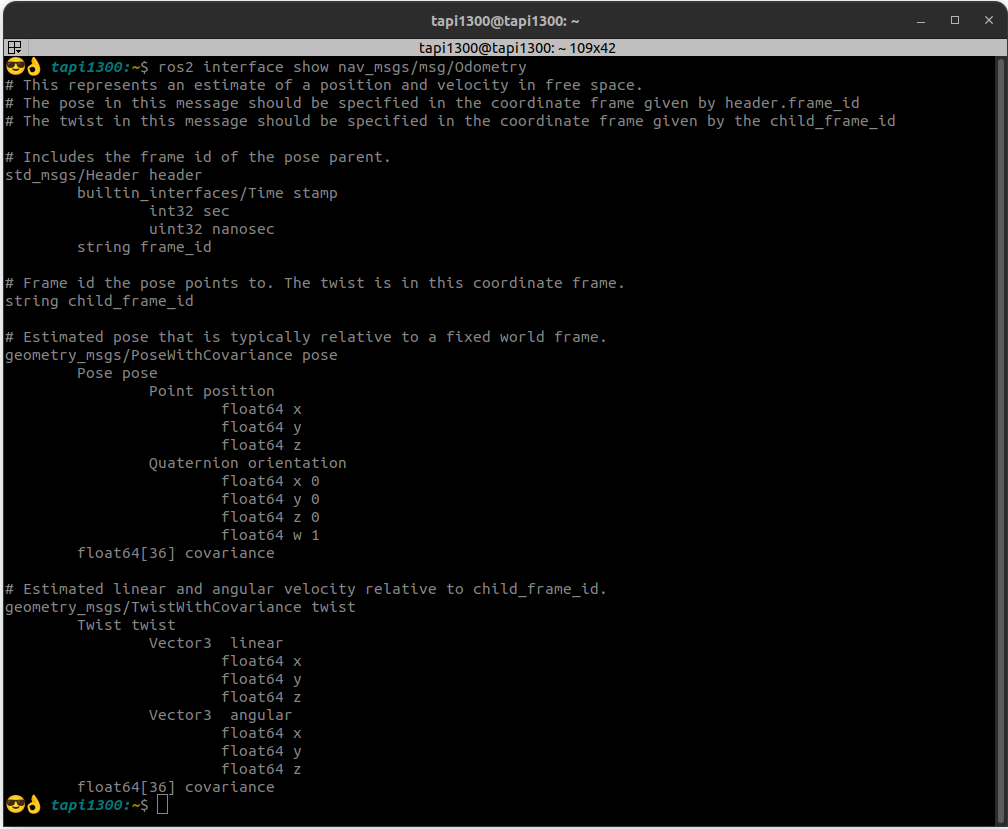
\includegraphics[width=12cm]{figs/c6/odom_msg.png}
    \end{center}
    \caption[Estructura mensaje Odometría]{Estructura del tipo de mensaje \textit{nav\_msgs/msg/Odometry}.}
    \label{fig:odom_struct}
\end{figure}

Los datos que se necesitan para la aplicación son la posición \textit{X} e \textit{Y}, al igual que la posición angular del eje \textit{Z}, por lo que esto será lo que se guarde en la
función \textit{callback} y lo que se envíe por el cable de salida usando un array formado por estos tres valores numéricos. Los primeros dos valores se pueden sacar
directamente del campo \textit{pose.pose.position} del mensaje, pero la rotación viene dada mediante cuaterniones, por lo que hay que transformarlo a ángulos de euler y obtener
el valor que se busca. Esto se realiza mediante la función \textit{Rotation} del paquete
\textit{scipy.spatial.transform}\footnote{\textbf{Librería Spicy}: \url{docs.scipy.org/doc/scipy/reference/generated/scipy.spatial.transform.Rotation.html}}
de \textit{python3}.
\begin{code}[H]
    \begin{lstlisting}[language=python]
        def callback(self, msg):
            global odom
            odom[0] = msg.pose.pose.position.x
            odom[1] = msg.pose.pose.position.y
            rot = Rotation.from_quat([msg.pose.pose.orientation.x, msg.pose.pose.orientation.y, msg.pose.pose.orientation.z, msg.pose.pose.orientation.w])
            odom[2] = rot.as_euler('xyz', degrees=True)[2]
    \end{lstlisting}
    \caption[Funciones para obtener la fuerza repulsiva]{Funciones para obtener la fuerza repulsiva.}
    \label{cod:rep_vel}
\end{code}

El siguiente bloque es el generador de destinos, que usa la ubicación del robot para comprobar si ha llegado a la actual (teniendo en cuenta un margen) y mandar
la siguiente dentro de la lista de destinos. También se ha implementado un contador de vueltas, aprovechando que se ha creado un circuito cerrado.

\begin{code}[H]
    \begin{lstlisting}[language=python]
        def main(inputs, outputs, parameters, synchronise):
            dest_arr = [[7,9],
                        [10,15],
                        [10,23],
                        [5,26],
                        [-1,23],
                        [-1,9]]
            destination = [0,0,0]
            odom = []
            first = True
            margen = 1
            actual = -1
            lap = 0
            while 1:
                odom = inputs.read_array("Odom")
                if odom is not None:
                    if(first or 
                            (odom[0] > dest_arr[actual][0]-margen and 
                            odom[0] < dest_arr[actual][0]+margen and
                            odom[1] > dest_arr[actual][1]-margen and 
                            odom[1] < dest_arr[actual][1]+margen)):
                        actual += 1
                        if(first or actual > len(dest_arr)-1):
                            lap +=1
                            actual = 0    
                            print("LAP NUMBER " + str(lap)) 
                        destination = dest_arr[actual]
                        outputs.share_array("Destination", destination)
                        print("NEW DESTINATION! " + str(destination))
                        first = False
    \end{lstlisting}
    \caption[Bloque generador de ubicaciones]{Bloque generador de ubicaciones.}
    \label{cod:dest_gen}
\end{code}

Estos dos \textit{arrays} (\textit{odom} y destino) los recibe el siguiente bloque, que es el que calcula la fuerza atractiva. Este bloque comprueba que
los datos que recibe no estén vacíos (al iniciar la ejecución puede leer \textit{null} de los cables), calculando la posición relativa del objetivo
respecto al robot tanto para los ejes \textit{X} e \textit{Y} como para la rotación relativa. En caso de que la rotación relativa supere un valor máximo,
se establece dicho máximo como valor de ángulo relativo, enviando éste como único valor, ya que en esta versión sólo se tiene en cuenta la velocidad angular,
manteniendo la lineal constante a 1 (en el VFF con máquina de estados sí se tiene en cuenta la velocidad lineal).

\begin{code}[H]
    \begin{lstlisting}[language=python]
        max_y_rel = 2
        def main(inputs, outputs, parameters, synchronise):
            while True:
                x_y_Yaw = inputs.read_array("Odom")
                dest = inputs.read_array("Destination")
                if x_y_Yaw is not None and dest is not None:
                    dx = dest[0] - x_y_Yaw[0]
                    dy = dest[1] - x_y_Yaw[1]
                    # Rotate with current angle
                    y_rel = dx * math.sin (math.radians(-x_y_Yaw[2])) + dy * math.cos (math.radians(-x_y_Yaw[2]))
                    if(y_rel > max_y_rel):
                        y_rel = max_y_rel
                    elif(y_rel < -max_y_rel):
                        y_rel = -max_y_rel
                    outputs.share_number("AttrForce", y_rel)
    \end{lstlisting}
    \caption[Bloque fuerza atractiva]{Bloque que calcula la fuerza atractiva.}
    \label{cod:attr_vel}
\end{code}

Por último, ambas fuerzas se combinan en un mismo bloque, que es el encargado de sumar ambas fuerzas y transformarlas en velocidad angular. Para ello aplica
un valor a modo de controlador constante para que la fuerza repulsiva sea más significativa que la atractiva y permitir que el robot esquive objetos que
puedan quedar muy cercanos. Finalmente se envía el \textit{array} de velocidades manteniendo la velocidad lineal a 1 y siendo la velocidad angular el valor
calculado por el algoritmo.

\begin{code}[H]
    \begin{lstlisting}[language=python]
        import math

        def main(inputs, outputs, parameters, synchronise):
            maximo = 3
            while True:            
                rep = inputs.read_number("RepForce")
                attr = inputs.read_number("AttrForce")
                if rep is not None and attr is not None:
                    final_w = 1.4*rep + 0.4*attr
                    if(final_w > maximo):
                        final_w = maximo
                    elif(final_w < -maximo):
                        final_w = -maximo
                    outputs.share_array("Vels", [1,0,0,0,0,final_w])
    \end{lstlisting}
    \caption[Bloque fuerzas a velocidades]{Bloque que transforma las fuerzas en velocidades.}
    \label{cod:VFF_force_to_vel}
\end{code}

\subsection{Validación experimental}
\label{subsec:val_exp_VFF}
Para comprobar que el algoritmo funcionase, se han realizado varias pruebas: sólo fuerza repulsiva con obstáculos y sin ellos, y el algoritmo completo con un
bloque de depuración (\ref{subsec:spec_bloques_FSM}).

Para las primeras pruebas el circuito contaría únicamente con 3 bloques: el bloque del sensor láser, el que calcula la fuerza repulsiva y el bloque MotorDriverROS2:

\begin{figure} [H]
    \begin{center}
        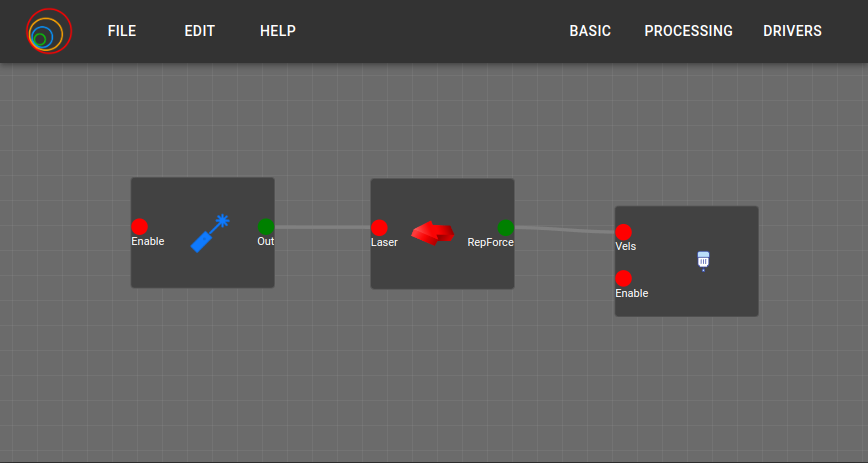
\includegraphics[width=9cm]{figs/c6/VFF_r_Circ.png}
    \end{center}
    \caption[Circuito VFF sólo fuerza repulsiva]{Circuito de VFF sólo con la fuerza repulsiva.}
    \label{fig:VFF_r_circ}
\end{figure}

Como podemos comprobar en las siguientes secuencias y en sus vídeos correspondientes, la parte de la fuerza repulsiva cumple con el objetivo, ya que mantiene
al robot alejado de las paredes del circuito a la vez que evita los obstáculos (en el caso en el que los hay).

\begin{figure} [H]
    \begin{center}
        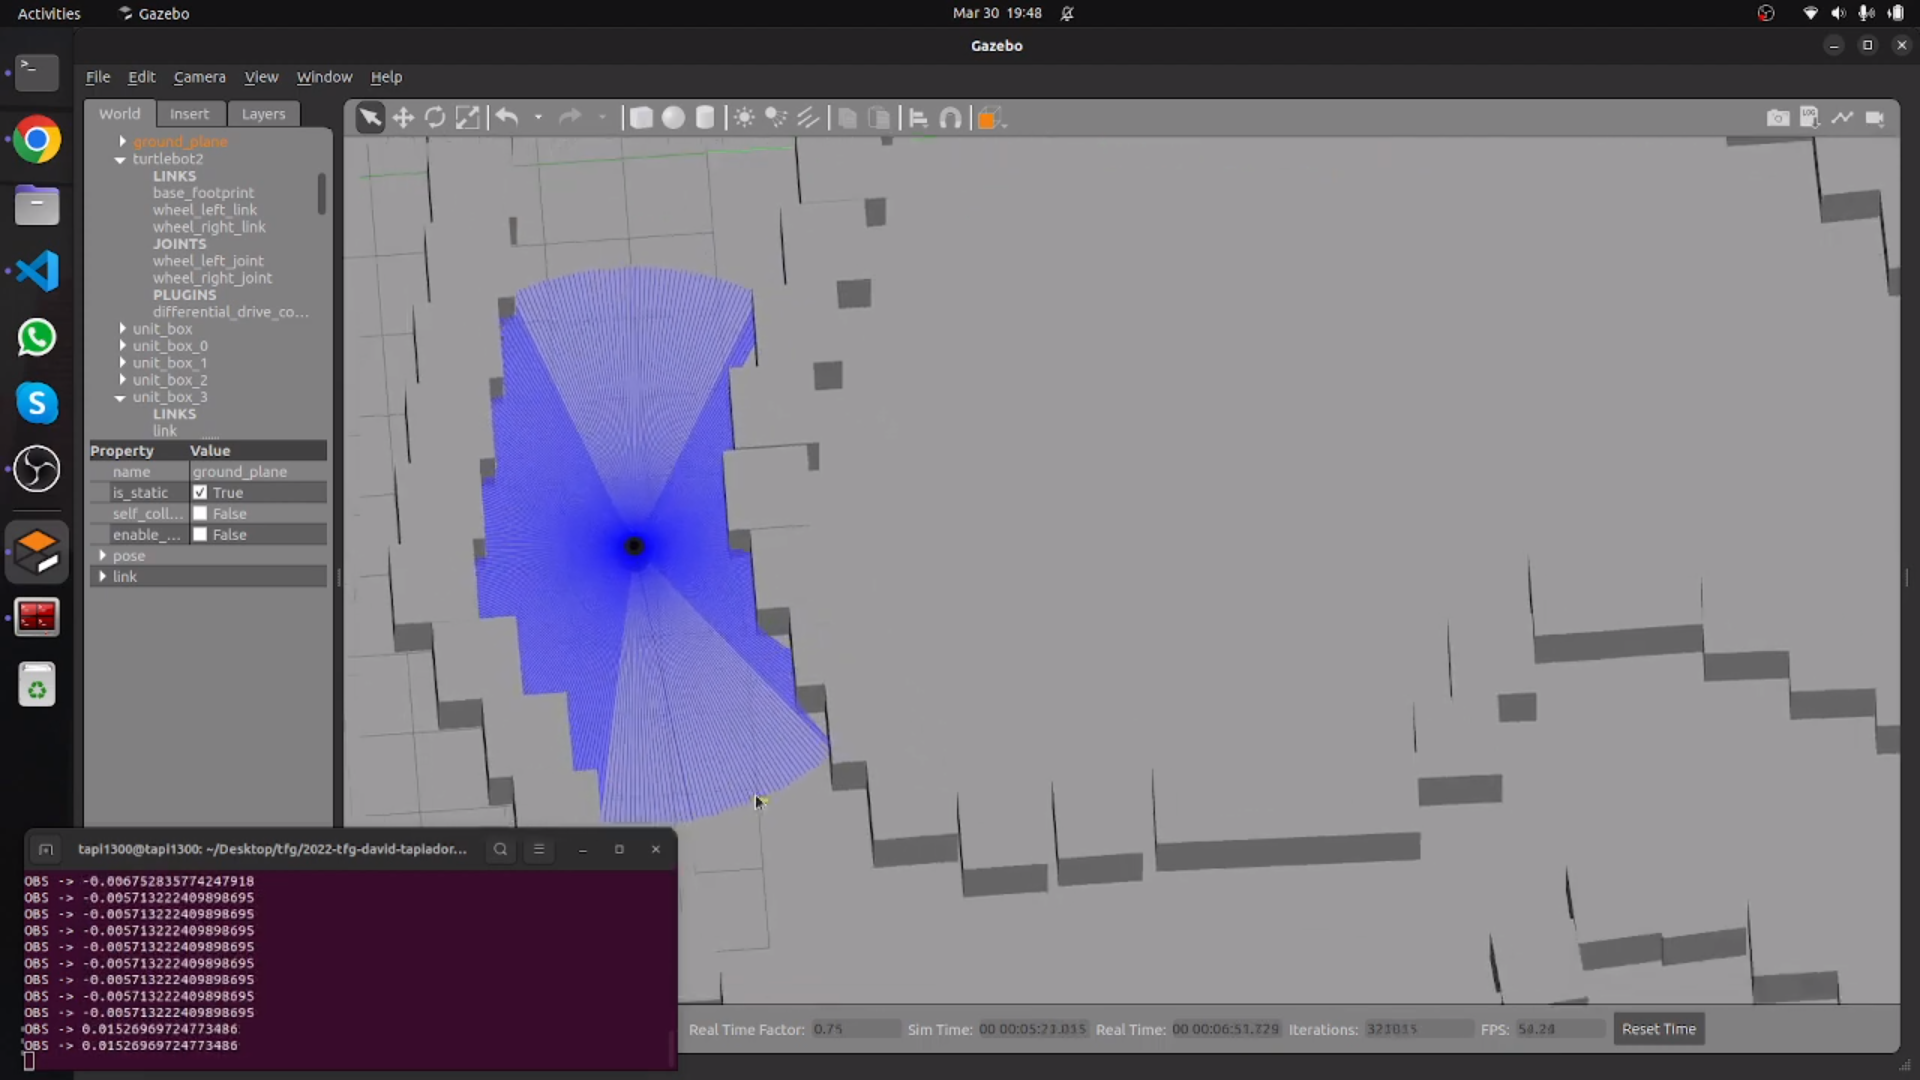
\includegraphics[width=7cm]{figs/c6/VFF_rs1.png}
        \includegraphics[width=7cm]{figs/c6/VFF_rs2.png}
    \end{center}
    \caption[Secuencia VFF fuerza repulsiva sin obstáculos]{VFF usando sólo la fuerza repulsiva sin obstáculos. Imagenes obtenidas de Youtube\footnotemark.}
    \label{fig:VFF_r_S}
\end{figure}
\footnotetext{\textbf{Vídeo VFF fuerza repulsiva sin obstáculos}: \url{https://www.youtube.com/watch?v=uhtBRw96Zl4&ab_channel=Tapii}}
\begin{figure} [H]
    \begin{center}
        \includegraphics[width=7cm]{figs/c6/VFF_rc1.png}
        \includegraphics[width=7cm]{figs/c6/VFF_rc2.png}
    \end{center}
    \caption[Secuencia bloque MotorDriverROS2 real]{VFF usando sólo la fuerza repulsiva con obstáculos. Imagenes obtenidas de Youtube\footnotemark.}
    \label{fig:MotordriverReal}
\end{figure}
\footnotetext{\textbf{Vídeo VFF fuerza repulsiva con obstáculos}: \url{https://www.youtube.com/watch?v=HeTFum_gTGw&ab_channel=Tapii}}

En la siguiente prueba, el circuito usado incluye el bloque display (se describirá su funcionamiento en el siguiente punto, ya que aquí no estaba completamente
desarrollado) y un bloque \textit{screen} para mostrar la imagen de este bloque.

\begin{figure} [H]
    \begin{center}
        \includegraphics[width=10cm]{figs/c6/VFF_disp_circ.png}
    \end{center}
    \caption[Circuito VFF]{Circuito del algoritmo VFF.}
    \label{fig:VFF_disp_circ}
\end{figure}

\begin{figure} [H]
    \begin{center}
        \includegraphics[width=7cm]{figs/c6/VFF_d1.png}
        \includegraphics[width=7cm]{figs/c6/VFF_d2.png}
    \end{center}
    \caption[Secuencia prueba VFF]{Secuencia de pruebas del algoritmo VFF. Imagenes obtenidas de Youtube\footnotemark.}
    \label{fig:VFF_pruebas}
\end{figure}
\footnotetext{\textbf{Vídeo VFF con display}: \url{https://www.youtube.com/watch?v=xdGCIrYFu7E&t=108s&ab_channel=Tapii}}

\section{VFF mediante máquina de estados}
\label{sec:FSM}

Una vez que el algoritmo está practicamente desarrollado, se va a implementar una máquina de estados. Esta máquina de estados tendrá 3 estados distintos: generar ubicación
aleatoria, ir a la ubicación y volver al punto de salida (después de varias ubicaciones aleatorias).\\

Como se puede ver en el siguiente diagrama, la ejecución se inicia
generando una ubicación aleatoria que se envía al estado VFF. Cuando se ha ido a 4 ubicaciones aleatorias, se pasa al estado "\textit{Return Home}", que envía la ubicación
inicial del robot como nuevo destino para el estado VFF. Una vez que llegue al inicio, se detiene al robot.

\begin{figure} [H]
    \begin{center}
        \includegraphics[width=10cm]{figs/c6/FSM_diag.png}
    \end{center}
    \caption[Diagrama máquina de estados]{Diagrama de la máquinas de estados.}
    \label{fig:FSM_diag}
\end{figure}

\subsection{Diseño del circuito y escenario}
\label{subsec:dis_bloques_FSM}

Para implementar el comportamiento de máquina de estados, se han implementado dos bloques nuevos para los comportamientos nuevos. También se ha colocado el bloque de la odometría
como un sensor general, ya que se usa en varios estados, mientras que el estado VFF está separado visualmente para que sea más sencillo de reconocer.

\begin{figure} [H]
    \begin{center}
        \includegraphics[width=13cm]{figs/c6/FSM_circuit.png}
    \end{center}
    \caption[Circuito VFF con FSM]{Circuito de VFF usando máquinas de estados.}
    \label{fig:FSM_circ}
\end{figure}

Como los objetivos ahora son aleatorios, no se puede usar el circuito que teníamos en el apartado anterior, por lo que se ha creado un mundo en el que se han
repartido varios cilindros por todo el mapa para que el robot tenga que moverse hasta el objetivo esquivándolos.

\begin{figure} [H]
    \begin{center}
        \includegraphics[width=13cm]{figs/c6/FSM_world.png}
    \end{center}
    \caption[Mundo VFF con FSM]{Mundo para probar el VFF con máquinas de estados.}
    \label{fig:FSM_world}
\end{figure}

\subsection{Bloques específicos}
\label{subsec:spec_bloques_FSM}

Para ampliar el funcionamiento del VFF para que también tenga en cuenta las fuerzas para calcular la velocidad lineal, se ha tenido que modificar los bloques que calculan las
fuerzas atractiva y repulsiva (\ref{cod:parse_laser_data} y \ref{cod:attr_vel}), por lo que en vez de mandar una única fuerza, se mandan la fuerza como vector (componente X e Y).
También se han añadido lecturas al \textit{input enable}, ya que es el que habilita activar y desactivar los bloques, únicamente ejecutando los bloques que estén activos en ese
momento y manteniendo el resto en estado inactivo.

\begin{code}[H]
    \begin{lstlisting}[language=python]
        # Cambio en bloque de fuerza repulsiva
        outputs.share_array("RepForce", [obsX/50, obsY/50])

        # Cambio en bloque de fuerza atractiva
        outputs.share_array("AttrForce", [x_rel, y_rel])

        # Bucle principal bloque laser
        while 1:
            enable = inputs.read_number('Enable')
            if enable == 1:
                measure = None
                rclpy.spin_once(laser_subscriber)
                if measure is not None:
                    outputs.share_array("Out",measure)  
    \end{lstlisting}
\end{code}

Uno de los bloques nuevos es el generador de ubicaciones aleatorias. Éste también es el que se encarga de decidir cuál será el siguiente estado. Para ello tiene un contador
interno que le permite saber cuántas veces se han generado ubicaciones aleatorias y, cuando se llegue al valor de \textit{max\_times} se cambia al estado de volver al origen.
Para generar la ubicación aleatoria, generamos un número que cumpla que num1 esté entre \textit{x-márgen} y \textit{x+márgen} y otro num2 que esté entre \textit{y-márgen} y \textit{y+márgen},
para evitar ubicaciones que estén demasiado alejadas del robot. También dicho número debe estar entre 0 y 30, ya que estos son los límites del mundo (máximo que se
representa dentro del bloque \textit{display}).

\begin{code}[H]
    \begin{lstlisting}[language=python]
    from random import randint
    import time

    def main(inputs, outputs, parameters, synchronise):
        first = True
        changed = False
        times = 0
        max_times = 4
        margen = 3
        x = [0,30]
        y = [0,30]
        while 1:    
                enable = inputs.read_number("Enable")
                if(enable == 0):
                    changed = False
    \end{lstlisting}
\end{code}
\begin{code}[H]
    \begin{lstlisting}[language=python]
                if (enable == 1 or first) and not changed:
                    odom = inputs.read_array("Odom")
                    if odom[0] != None:
                        changed = True
                        first = False
                        times += 1
                        if(times < max_times):
                            print("***ESTADO ACTIVADO -> GENERAR UBICACION ALEATORIA***")
                            dest = [randint(x[0]+1, x[1]-1),
                                        randint(y[0]+1,y[1]-1)]

                            while dest[0] > int(odom[0]-margen) and dest[0] < int(odom[0]+margen):
                                dest[0] = randint(x[0]+1, x[1]-1)
                            while dest[1] > int(odom[1]-margen) and dest[1] < int(odom[1]+margen):
                                dest[1] = randint(y[0]+1,y[1]-1)
                                
                            print("NUEVO DESTINO -> " + str(dest))
                            time.sleep(2)
                            print("***ESTADO ACTIVADO -> VFF***")
                            outputs.share_array("Dest", dest)
                            outputs.share_number("Next", 1)
                            outputs.share_number("Last", 0)
                        else:
                            print("***ESTADO ACTIVADO -> VUELTA AL ORIGEN***")
                            outputs.share_number("Next", 0)
                            outputs.share_number("Last", 1)
    \end{lstlisting}
    \caption[Bloque generador aleatorio de destinos]{Bloque que genera destinos aleatorios y decide el siguiente estado.}
    \label{cod:FSM_asker}
\end{code}

El siguiente bloque nuevo es el correspondiente al estado de volver al inicio. Cuando este bloque se activa, envía la ubicación del origen al estado VFF e imprime
varias trazas para saber en qué punto del comportamiento se encuentra la ejecución.

\begin{code}[H]
    \begin{lstlisting}[language=python]
        import time
        def main(inputs, outputs, parameters, synchronise):
            dest = [2,10]
            first = True
            going = False
            while 1:
                enable = inputs.read_number("Enable")
                if enable == 1 and first:
                        print("UBICACION DEL ORIGEN -> " + str(dest))
                        time.sleep(2)
                        outputs.share_array("Dest", dest)
                        outputs.share_number("Next", 1)
                        first = False
                if enable == 0 and not first:
                    going = True
                if enable == 1 and going:
                    print("HEMOS LLEGADO AL ORIGEN!!")
                    outputs.share_number("Next", 0)
    \end{lstlisting}
    \caption[Bloque return home]{Bloque para volver al inicio.}
    \label{cod:FSM_return_home}
\end{code}

El bloque que transforma las fuerzas a velocidades también cambia, ya que ahora hay que tener en cuenta la componente lineal de las fuerzas y, por lo tanto, calcular nuevas
proporciones y evaluar valores máximos y mínimos. También se ha añadido que, si la velocidad lineal es negativa y la angular es cercana a 0 (valor absoluto menor que 0.3), se
ponga al robot a girar estático. Esto es para evitar objetivos que se encuentren detrás del robot y que, por lo tanto, intente llegar a ellos marcha atrás.

\begin{code}[H]
    \begin{lstlisting}[language=python]
        def main(inputs, outputs, parameters, synchronise):
            max_v = 2
            min_v = 0.5
            max_w = 3
            alpha_V = 1
            beta_V = 1
            alpha_W = 0.7
            beta_W = 1.4
            while 1:
                rep = inputs.read_array("RepForce")
                attr = inputs.read_array("AttrForce")
                if rep is not None and attr is not None:
                    attr_x, attr_y = test_max(attr[0],attr[1])
                    rep_x, rep_y = test_max(rep[0],rep[1])
                    final_v = alpha_V*attr_x + beta_V*rep_x
                    final_w = alpha_W*attr_y + beta_W*rep_y
    \end{lstlisting}
\end{code}
\begin{code}[H]
    \begin{lstlisting}[language=python]
                    if(final_v < 0 and final_w < 0.3 and final_w > 0.3):
                        # Rotar en el sitio hasta que no sea sentido opuesto
                        final_v = 0
                        final_w = max_w/3
                    elif(final_v > max_v):
                        final_v = max_v
                    elif(final_v < min_v):
                        final_v = min_v

                    if(final_w > max_w):
                        final_w = max_w
                    elif(final_w < -max_w):
                        final_w = -max_w

                    outputs.share_array("Vels", [final_v,0,0,0,0,final_w])
    \end{lstlisting}
    \caption[Bloque forces to vels]{Bloque que pasa de fuerzas a velocidades.}
    \label{cod:FSM_forcestovels}
\end{code}

Por último, el bloque \textit{display} consiste en crear una imagen mediante un \textit{array} de \textit{numpy} en el que se muestra aproximadamente una representación del
mundo que ve el robot. Aquí se muestran tanto la ubicación del robot y del destino, como las fuerzas atractiva (verde), repulsiva (roja) y total (naranja), sus valores y las lecturas
del láser mediante pequeños puntos. También se ha representado cada metro cuadrado del simulador mediante una cuadrícula en la imagen.

Aquí se usa la librería cv2 de opencv-python\footnote{\textbf{OpenCV-Python}: \url{https://pypi.org/project/opencv-python/}} para editar la imágen, para insertar
líneas (\textit{cv2.line} para líneas y \textit{cv2.arrowedLine} para flechas) y para escribir texto (\textit{cv2.putText}), al igual que la librería \textit{math}
(\textit{cos}, \textit{sin}, \textit{radians}, \textit{sqrt}, ...) para calcular la orientación de las flechas de las distintas fuerzas.

Dada la extensión del código, no se va a incluir en esta memoria, por lo que
aquí\footnote{\textbf{Código bloque display}: \url{https://github.com/RoboticsLabURJC/2022-tfg-david-tapiador/blob/main/FSM/ZIPS/FSM_final/modules/Code_1.py}}
se puede acceder a él.

\subsection{Validación experimental}
\label{subsec:val_exp_FSM}

En la siguiente secuencia de imágenes se puede comprobar el resultado de la ejecución del algoritmo usando la máquina de estados. Como se puede ver, el TurtleBot2 es capaz de
evitar los obstáculos en tiempo real llegando a los distintos objetivos aleatorios que se han calculado durante esa ejecución.

\begin{figure} [H]
    \begin{center}
        \includegraphics[width=7cm]{figs/c6/FSM_final1.png}
        \includegraphics[width=7cm]{figs/c6/FSM_final2.png}
        \includegraphics[width=7cm]{figs/c6/FSM_final3.png}
        \includegraphics[width=7cm]{figs/c6/FSM_final4.png}
    \end{center}
    \caption[Secuencia VFF con FSM]{Secuencia de imágenes del algoritmo VFF usando FSM. Imagenes obtenidas de Youtube\footnotemark.}
    \label{fig:sec_FSM_final}
\end{figure}
\footnotetext{\textbf{Vídeo}: \url{https://www.youtube.com/watch?v=EiBT8yqX29Q&ab_channel=Tapii}}







\chapter{Conclusiones}
\label{cap:capitulo7}

Finalizamos esta memoria de Trabajo Fin de Grado con un resumen de las metas logradas por este trabajo al igual que por posibles líneas de trabajo para continuar.

\section{Conclusiones}


\clearpage
\thispagestyle{empty}

\printindex \nocite{*}
\appendix
\bibliographystyle{apalike} \bibliography{bibliografia}

\end{document}
































